\documentclass[]{article}


\input{H_structue}
\usepackage[a4paper, margin=1.2in]{geometry}
\definecolor{cover}{RGB}{230, 194, 24}

\begin{document}


%----------------------------------------------------------------------------------------
%	TITLE PAGE
%----------------------------------------------------------------------------------------
\begingroup
\AddToShipoutPicture*{\put(0,0){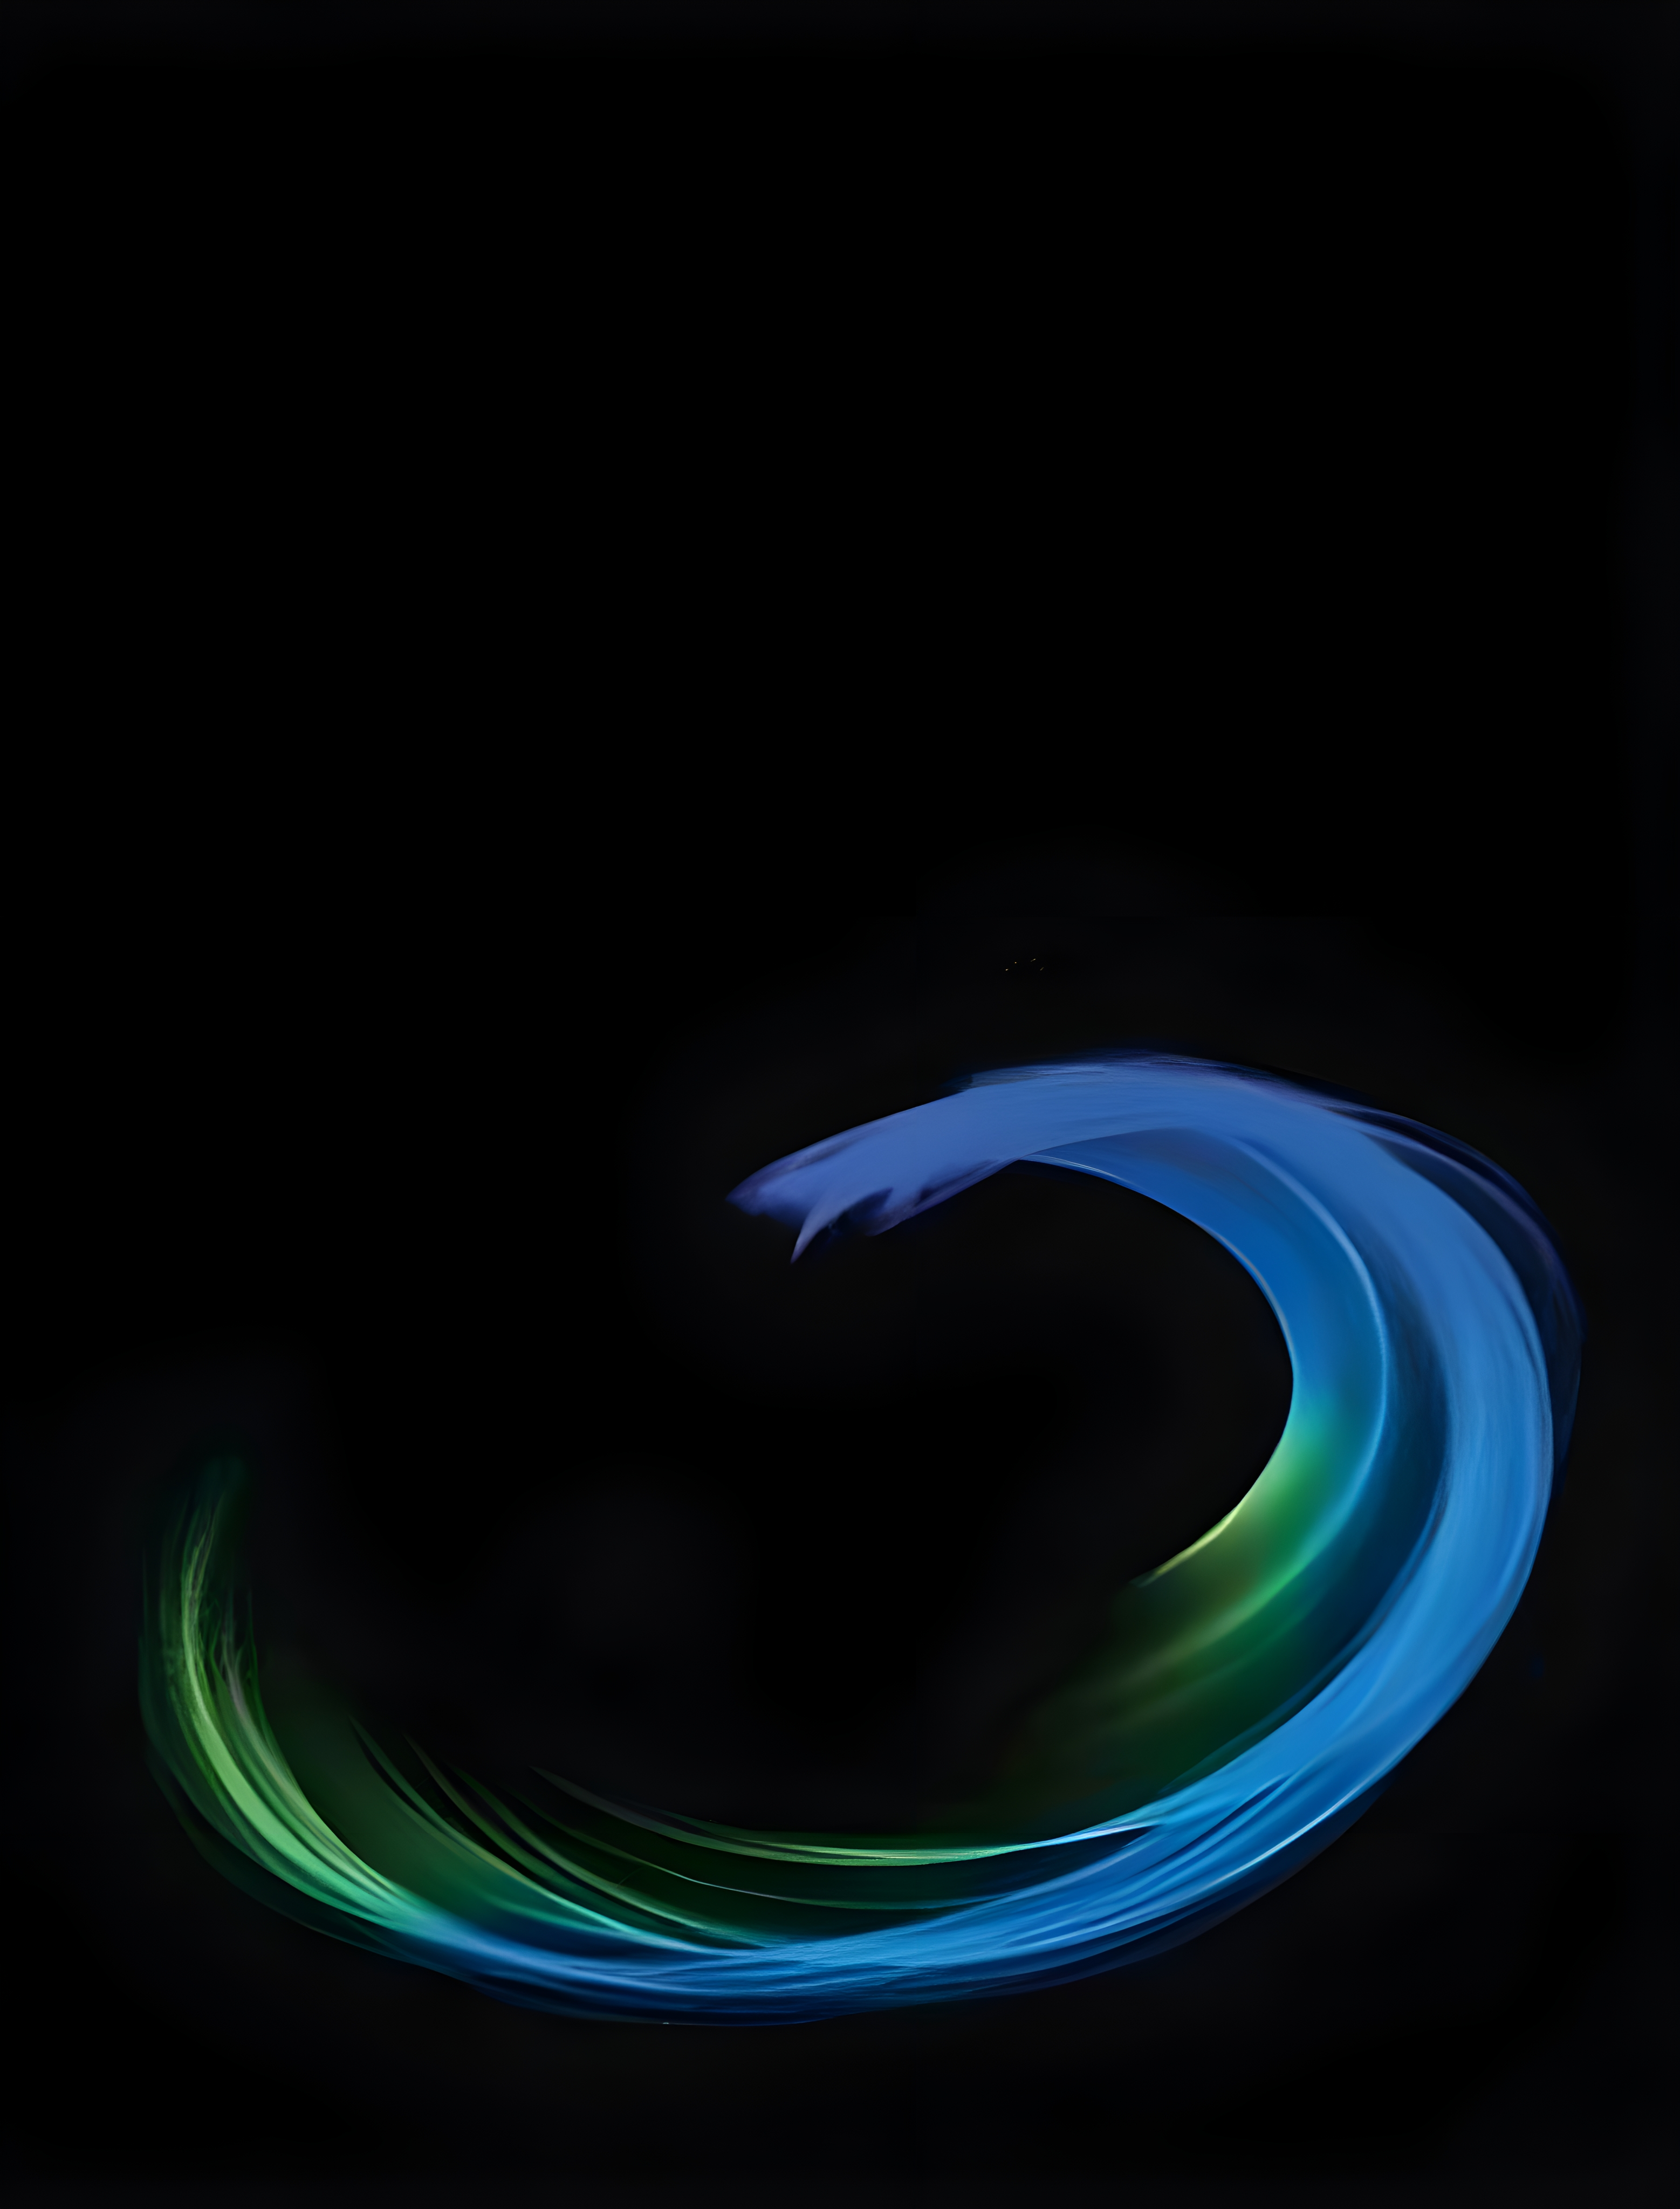
\includegraphics[width=\paperwidth,height=\paperheight]{Cover1.jpg}}}
\par\sffamily\selectfont
\color{cover}
\fontsize{80pt}{0}\selectfont Partial\par
\fontsize{80pt}{0}\selectfont Differential\par
\fontsize{80pt}{0}\selectfont Equations\par
\begin{center}
    {\LARGE 01356 Spring 2023}\par
    \vspace*{1cm}
    {\Huge Lecture Notes}\par       
\end{center}
\color{white}
\vspace*{4.5cm}
\fontsize{22pt}{0}\selectfont Lecturer: Prof. Mahmoud M. El-Borai\par
\fontsize{22pt}{0}\selectfont Prepared by: Ossama Abdelwahed And\par
\hspace*{4cm}
\fontsize{22pt}{0}\selectfont Ahmed.M.Habib\par
\endgroup

\newpage

\tableofcontents

\newpage

\section{Introduction}
The main goal of many scientific disciplines can be summarized to the following:

\begin{enumerate}
\item Formulate a set of mathematical equations to model a phenomena of interest
\item Analyze solutions to these equations in order to extract information and make predictions.
\end{enumerate}

The result of 1 is often a system of partial differential equations, thus the second becomes solving those partial differential equations.
\par
A partial differential equation (PDE) is is a differential equation containing partial derivatives of the dependent variable with respect to more than one independent variable.

\subsection{Order of PDE}
The order of a PDE is determined by the highest derivative in the equation.
\begin{align*}
\frac{\partial u}{\partial t} + {(\frac{\partial u}{\partial x})}^2 &= 0 \ \ \ \ \Longrightarrow  \text{First order}
\\
\frac{\partial^4 u}{\partial y^4} + \frac{\partial u}{\partial x} &= c \ \ \ \ \Longrightarrow  \text{Fourth order}
\end{align*}
do not mistake the order of the PDE with its degree, the degree of the PDE is the highest exponent appearing in the equation.
\subsection{Linearity} 
A linear PDE is one that is of first degree in all of its field variables and partial derivatives.
\begin{align*}
\frac{\partial u}{\partial t} + \frac{\partial u}{\partial x} &= 0 \dquad \text{linear}
\\
\frac{\partial^4 u}{\partial y^4} + \frac{\partial u}{\partial x} &= y \dquad \text{linear}
\\
\frac{\partial u}{\partial t} + {(\frac{\partial u}{\partial x})}^2 &= 0 \dquad \text{nonlinear}
\\
\frac{\partial^3 u}{\partial x^3} + {(\frac{\partial^2 u}{\partial y^2})}^5 &= \sin(x) \dquad \text{nonlinear}
\end{align*}

a linear operator can be defined for any linear equation, taking the first equation in the previous list, the linear operator $L$ can be defined as.
\[
L = \frac{\partial }{\partial t} + \frac{\partial u}{\partial x}
\]
and the equation can be written as.
\[
    L(u)=0    
\]

\subsection{Homogeneity}
Let $L$ be a linear operator. Then a linear partial differential equation can be written in the form.
\[
    L(u) = f(x_1,x_2, \dots , t)    
\]
if $f = 0$ then the equation is homogeneous, otherwise it is in-homogeneous.
\begin{align*}
\frac{\partial u}{\partial t} + \frac{\partial u}{\partial x} &= 0 \dquad \text{homogeneous}
\\
\frac{\partial^4 u}{\partial y^4} + \frac{\partial u}{\partial x} &= y \dquad \text{inhomogeneous}
\end{align*}

\newpage

\subsection{Boundary Conditions}
\
\begin{definition}[Boundary Conditions]
    Boundary conditions are constraints necessary for the solution of a boundary value problem.
\end{definition}
\begin{definition}[Boundary Value Problem]
    BVP is a differential equation to be solved in a domain on whose boundary the function is known.
\end{definition}
We will be interested in one type of boundary conditions in this course which is the Drichlet Conditions, specifies the value that the unknown function needs to take on along the boundary of the domain. For example, the Laplace equation on a circle with drichlet condition will be.
\[
    \nabla^2 u(x) = 0 \quad \forall x \in G    
\]
\[
    u(x) = f(x) \quad \forall x \in G    
\]
\begin{center}
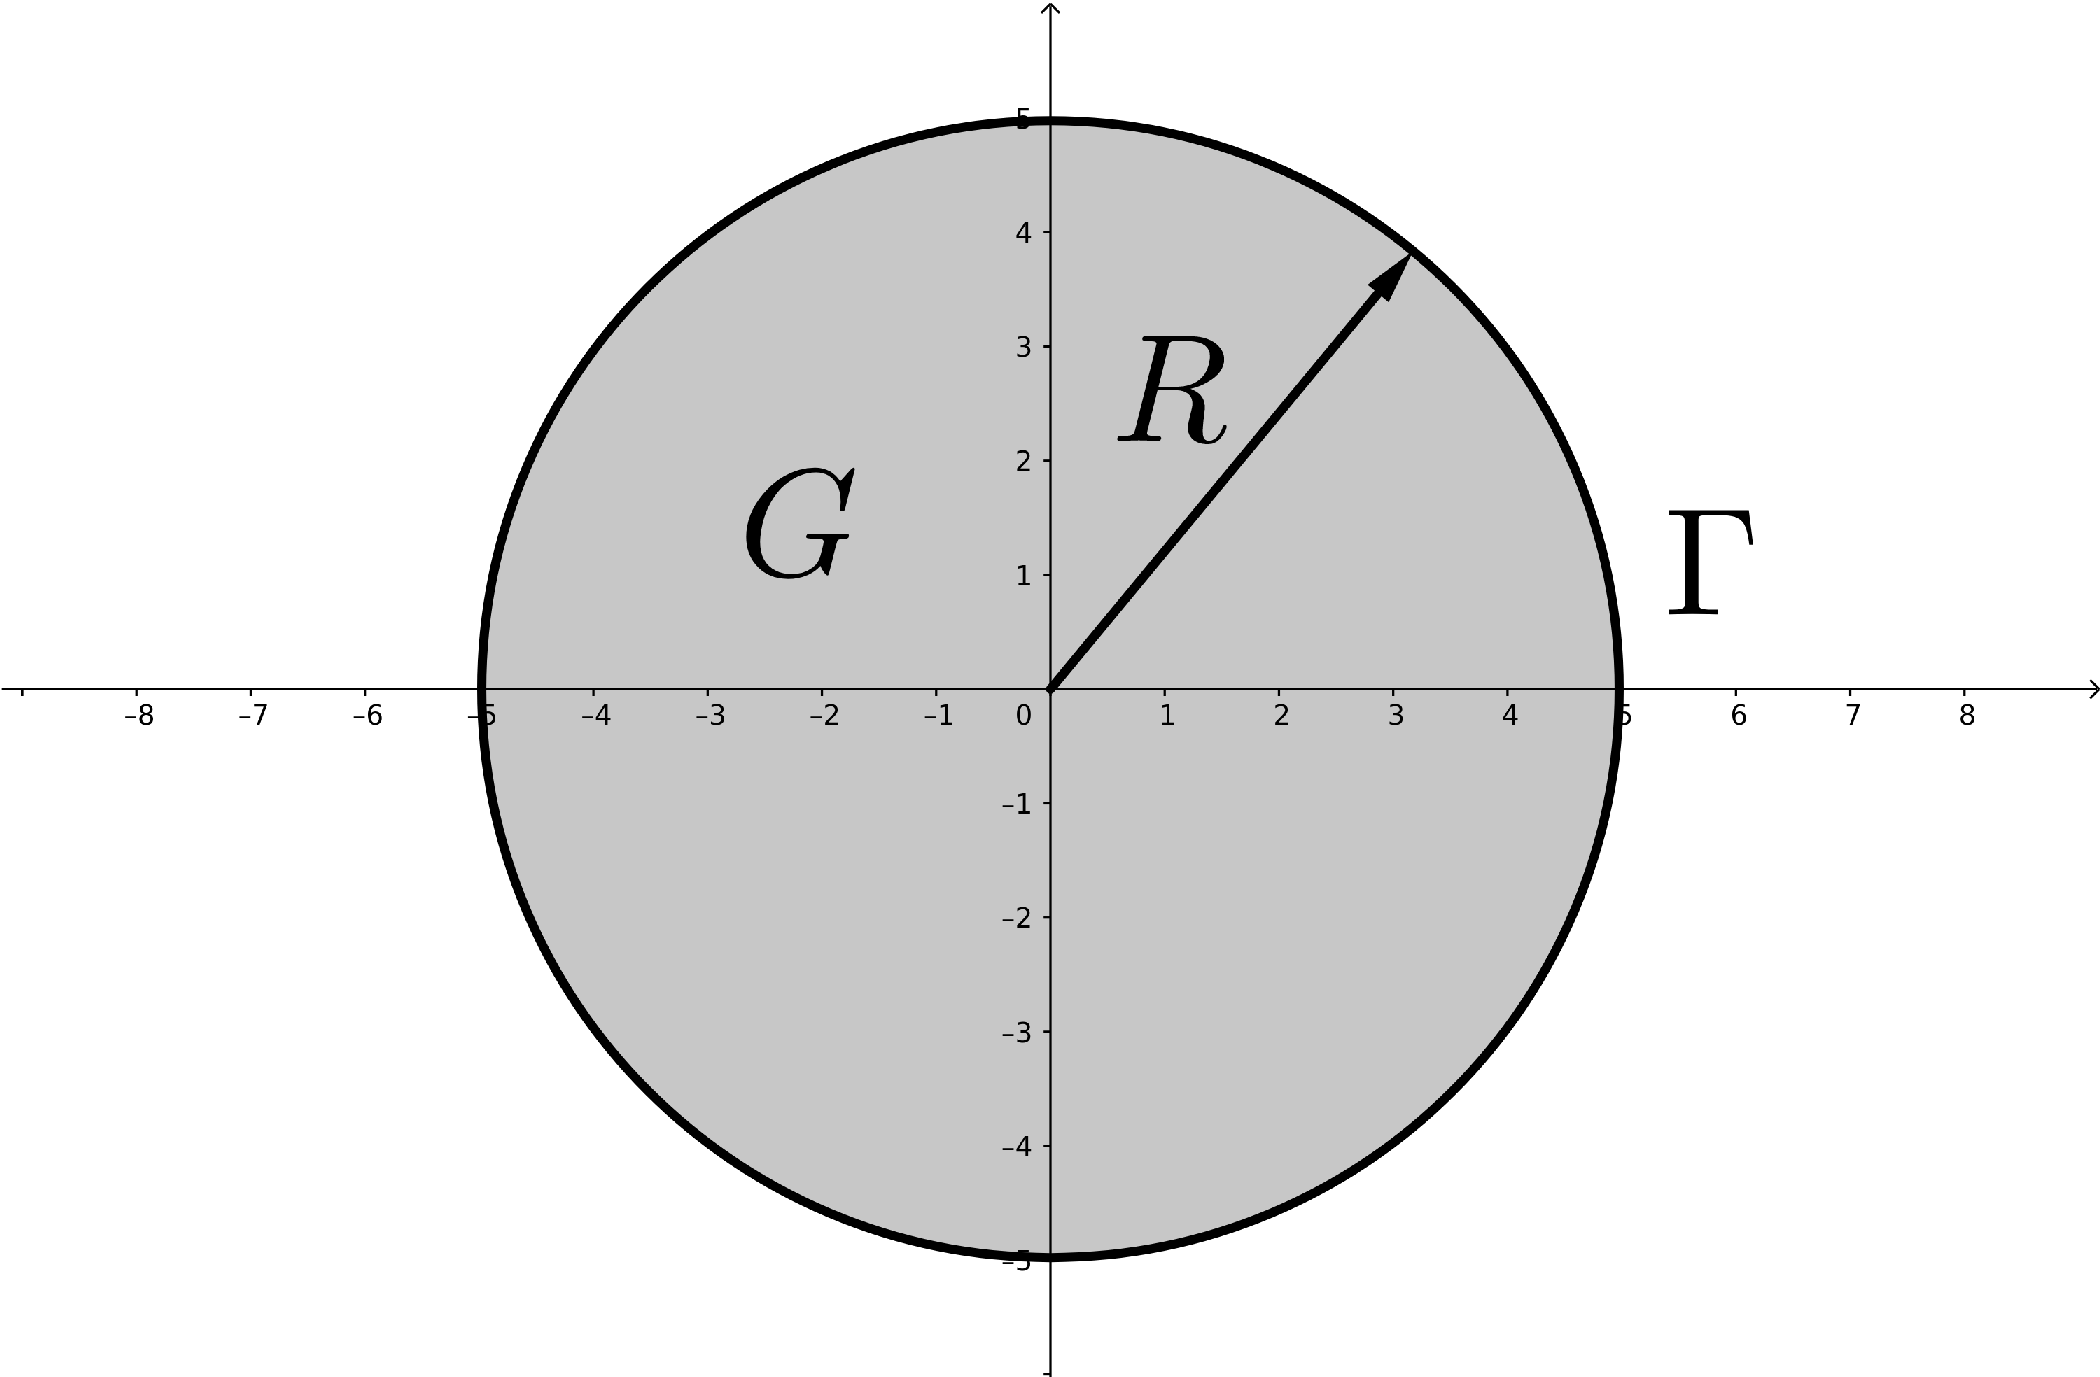
\includegraphics[scale=0.1]{laplacecircle.png} 
\end{center}
\[
    G = \left\lbrace (x,y):x^2+y^2 < R^2 \right\rbrace  \;\;\;\;\;\;\;\;\;\ \Gamma = \left\lbrace (x,y):x^2+y^2 = R^2 \right\rbrace    
\]
\begin{definition}[Drichlet problems]
    are problems that has only boundary conditions
\end{definition}
\subsection{Initial Condition}
\
\begin{definition}[The initial condition]
    is a condition that a solution must have at only on instant of time, which is the starting time as it can be found experimentally.
\end{definition}
An example is the heat equation with initial condition.
\[
    \frac{\partial u(x,t)}{\partial t}  = c^2 \frac{\partial u(x,t)}{\partial x}
\]
\[
    u(x,0) = f(x)
\]
\begin{definition}[Cauchy problems]
    are problems that has only initial conditions
\end{definition}
\subsection{Equations of Mathematical Physics}
The most frequently encountered equations in physics are the following
\begin{enumerate}
\item Heat Equation
\[
    \frac{\partial u(x,t)}{\partial t} = c^2 \frac{\partial^2 u(x,t)}{\partial x^2}    
\]
\item Wave Equation 
\[
    \frac{\partial^2 u(x,t)}{\partial t^2} = c^2 \frac{\partial^2 u(x,t)}{\partial x^2}    
\]
\item Laplace's Equation
\[
    \nabla^2 u(x) = \frac{\partial^2 u(x)}{\partial x^{2}_{1}} + \frac{\partial^2 u(x)}{\partial x^{2}_{2}} + \frac{\partial^2 u(x)}{\partial x^{2}_{3}} + \cdots = 0    
\]
\end{enumerate}

\newpage

\section{Canonical Form}
Consider the following PDE with variable coefficients. We are aiming to transform this equation into its canonical form
\begin{equation}
A\left(x,y\right)\frac{\partial^2 u\left(x,y\right)}{\partial x^2} + 2B\left(x,y\right)\frac{\partial^2 u\left(x,y\right)}{\partial x\partial y}+C\left(x,y\right)\frac{\partial^2 u\left(x,y\right)}{\partial y^2}+F\left(x,y,u,\frac{\partial u}{\partial x},\frac{\partial u}{\partial y}\right) = 0
\end{equation}
The first three terms are called the principle terms and the last term is called the Young term (Y.T) which does not contain second order derivatives of u.
\par
We start by preforming a change of variables such that.
\[
    \xi = \xi\left(x,y\right),\dquad \eta = \eta\left(x,y\right)    
\]
taking into consideration the Jacobian of the transformation
\[
    J =\begin{vmatrix} \frac{\partial\xi}{\partial x}  \;\;\; \frac{\partial\eta}{\partial x} \\ \\ \frac{\partial\xi}{\partial y}\;\;\; \frac{\partial\eta}{\partial y} \end{vmatrix} \neq 0    
\]
Then we find our derivatives.
\begin{align*}
\frac{\partial u}{\partial x} &= \frac{\partial u}{\partial\xi}\frac{\partial\xi}{\partial x}+\frac{\partial u}{\partial\eta}\frac{\partial\eta}{\partial x}
\\
\frac{\partial^2 u}{\partial x^2} &= \frac{\partial u}{\partial\xi}\frac{\partial^2\xi}{\partial x^2}+\frac{\partial\xi}{\partial x}\left[\frac{\partial^2 u}{\partial\xi^2}\frac{\partial\xi}{\partial x}+\frac{\partial^2 u}{\partial\eta\partial\xi}\frac{\partial\eta}{\partial x}\right]+\frac{\partial u}{\partial\eta}\frac{\partial^2\eta}{\partial x^2}+\frac{\partial\eta}{\partial x}\left[\frac{\partial^2 u}{\partial\eta^2}\frac{\partial\eta}{\partial x}+\frac{\partial^2 u}{\partial\eta\partial\xi}\frac{\partial\xi}{\partial x}\right]
\end{align*}

adding similar terms and simplifying

\begin{equation}
\frac{\partial^2 u}{\partial x^2} = {(\frac{\partial\xi}{\partial x})}^2\frac{\partial^2 u}{\partial\xi^2}+2\frac{\partial\xi}{\partial x}\frac{\partial\eta}{\partial x}\frac{\partial^2 u}{\partial\eta\partial\xi}+{(\frac{\partial\eta}{\partial x})}^2\frac{\partial^2 u}{\partial\eta^2}+Y.T
\end{equation}

and in similar fashion we can get.

\begin{equation}
\frac{\partial^2 u}{\partial y^2} = {(\frac{\partial\xi}{\partial y})}^2\frac{\partial^2 u}{\partial\xi^2}+2\frac{\partial\xi}{\partial y}\frac{\partial\eta}{\partial y}\frac{\partial^2 u}{\partial\eta\partial\xi}+{(\frac{\partial\eta}{\partial y})}^2\frac{\partial^2 u}{\partial\eta^2}+Y.T
\end{equation}

\begin{equation}
\frac{\partial^2 u}{\partial y\partial x} = \frac{\partial\xi}{\partial x}\frac{\partial\xi}{\partial y}\frac{\partial^2 u}{\partial\xi^2}+\left[\frac{\partial\xi}{\partial x}\frac{\partial\eta}{\partial y}+\frac{\partial\xi}{\partial y}\frac{\partial\eta}{\partial x}\right]\frac{\partial^2 u}{\partial\xi\partial\eta}+\frac{\partial\eta}{\partial x}\frac{\partial\eta}{\partial y}\frac{\partial^2 u}{\partial\eta^2} + Y.T
\end{equation}

substituting (2), (3), and (4) in (1) we get.
\begin{align*}
       A&\left[{(\frac{\partial\xi}{\partial x})}^2\frac{\partial^2 u}{\partial\xi^2}+2\frac{\partial\xi}{\partial x}\frac{\partial\eta}{\partial x}\frac{\partial^2 u}{\partial\eta\partial\xi}+{(\frac{\partial\eta}{\partial x})}^2\frac{\partial^2 u}{\partial\eta^2}\right]
    \\ +2B&\left[\frac{\partial\xi}{\partial x}\frac{\partial\xi}{\partial y}\frac{\partial^2 u}{\partial\xi^2}+\left[\frac{\partial\xi}{\partial x}\frac{\partial\eta}{\partial y}+\frac{\partial\xi}{\partial y}\frac{\partial\eta}{\partial x}\right]\frac{\partial^2 u}{\partial\xi\partial\eta}+\frac{\partial\eta}{\partial x}\frac{\partial\eta}{\partial y}\frac{\partial^2 u}{\partial\eta^2}\right] 
    \\ +C&\left[{(\frac{\partial\xi}{\partial y})}^2\frac{\partial^2 u}{\partial\xi^2}+2\frac{\partial\xi}{\partial y}\frac{\partial\eta}{\partial y}\frac{\partial^2 u}{\partial\eta\partial\xi}+{(\frac{\partial\eta}{\partial y})}^2\frac{\partial^2 u}{\partial\eta^2}\right]+Y.T =0    
\end{align*}
rearranging terms.
\begin{align*}
\left[A{(\frac{\partial\xi}{\partial x})}^2+2B\frac{\partial\xi}{\partial x}\frac{\partial\xi}{\partial y}+C{(\frac{\partial\xi}{\partial y})}^2\right]\frac{\partial^2 u}{\partial\xi^2}+\left[A{(\frac{\partial\eta}{\partial x})}^2+2B\frac{\partial\eta}{\partial x}\frac{\partial\eta}{\partial y}+C{(\frac{\partial\eta}{\partial y})}^2\right]\frac{\partial^2 u}{\partial\eta^2}\\
+\left[2A\frac{\partial\xi}{\partial x}\frac{\partial\eta}{\partial x}+2B\left[\frac{\partial\xi}{\partial x}\frac{\partial\eta}{\partial y}+\frac{\partial\xi}{\partial y}\frac{\partial\eta}{\partial x}\right]+2C\frac{\partial\xi}{\partial y}\frac{\partial\eta}{\partial y}\right]\frac{\partial^2 u}{\partial\eta\partial\xi}+Y.T=0
\end{align*}
we now try to find $\xi$ and $\eta$ such that.
\[
    \left[A{(\frac{\partial\xi}{\partial x})}^2+2B\frac{\partial\xi}{\partial x}\frac{\partial\xi}{\partial y}+C{(\frac{\partial\xi}{\partial y})}^2\right] =0    
\]
\[
    \left[A{(\frac{\partial\eta}{\partial x})}^2+2B\frac{\partial\eta}{\partial x}\frac{\partial\eta}{\partial y}+C{(\frac{\partial\eta}{\partial y})}^2\right]=0    
\]

we notice that both equations are the same quadratic equation, thus we solve for one of them to find both $\xi$ and $\eta$, we choose the first one and start by dividing the equation by ${(\frac{\partial\xi}{\partial y})}^2$.
\[
    A\frac{{(\frac{\partial\xi}{\partial x})}^2}{{(\frac{\partial\xi}{\partial y})}^2}+2B\frac{\left(\frac{\partial\xi}{\partial x}\right)}{\left(\frac{\partial\xi}{\partial y}\right)}+C =0    
\]
\[
    A{(\frac{\partial y}{\partial x})}^2-2B\frac{\partial y}{\partial x}+C =0    
\]

now using the quadratic formula to solve for $\frac{\partial y}{\partial x}$.

\[
    \frac{\partial y}{\partial x} = \frac{-\left(-2B\right)\pm\sqrt{{(-2B)}^2 -4AC}}{2A} = \frac{B\pm\sqrt{B^2 -AC}}{A}    
\]

this is called the characteristic equation.

\begin{enrichment*}{Equations Classification}
Equations are classified based on the value of the expression under the root

$B^2 > AC \;\;\;\;\;\; \forall x,y\in G$, Hyperbolic PDE (the general case of the wave equation) 

$B^2 < AC \;\;\;\;\;\; \forall x,y\in G$, Elliptic PDE (the general case of the Laplace equation) 

$B^2 = AC \;\;\;\;\;\; \forall x,y\in G$, Parabolic PDE (the general case of the Heat equation) 
\end{enrichment*}


\subsection{Examples}

\begin{example}
    Transform to the canonical form.
    \[
        4y^2\frac{\partial^2 u}{\partial x^2}-e^{2x}\frac{\partial^2 u}{\partial y^2}+\underbrace{6y^3}_{\text{Y.T}} = 0    
    \]
    \begin{center}
        ------ \textcolor{Solution}{Solution} ------ 
    \end{center}
    we start by determining the functions A,B, and C.
    \[
        A\left(x,y\right)=4y^2 \quad,\quad B\left(x,y\right)=0 \;\;\;,\;\;\; C\left(x,y\right)=-e^{2x}    
    \]
    we conclude from this that it has the form of a Hyperbolic PDE.
    \[
        B^2 =0 \quad>\quad AC=-4y^2e^{2x}, \quad \forall y\neq0,\quad \forall x    
    \]
    now we use the characteristic equation to determine the value of $\xi$ and $\eta$.
    \begin{align*}
        \frac{\partial y}{\partial x} &= \frac{B\pm\sqrt{B^2 -AC}}{A}\\
        \\
        &= \frac{\pm\sqrt{4y^2 e^{2x}}}{4y^2}=\pm\frac{e^x}{2y}
    \end{align*}
    rearranging and integrating.
    \begin{align*}
        2ydy &= \pm e^x dx
        \\
        \int 2ydy &= \pm \int e^x dx
        \\ \hspace{6cm}
        y^2 &= \pm e^x + constant \quad \Longrightarrow \quad y^2 \pm e^x = constant 
    \end{align*}
    we now set $\xi$ and $\eta$.
    \[
        \xi = e^x + y^2 \quad , \quad \eta = e^x - y^2    
    \]
    we now work out the derivatives.
    \begin{align*}
        \hspace{5cm}
        \frac{\partial u}{\partial x} &= \frac{\partial u}{\partial\xi}\frac{\partial\xi}{\partial x} + \frac{\partial u }{\partial\eta}\frac{\partial\eta}{\partial x}
        \\
        &= \frac{\partial u}{\partial\xi}e^x+\frac{\partial u}{\partial\eta}e^x
        \\
        \frac{\partial^2 u}{\partial x^2} &= e^x\left[\frac{\partial^2 u}{\partial\xi^2} e^x + \frac{\partial^2 u}{\partial\eta\partial\xi}e^x\right]+e^x\left[\frac{\partial^2 u}{\partial\eta^2} e^x + \frac{\partial^2 u}{\partial\xi\partial\eta}e^x\right]+Y.T
        \\
        &= e^{2x}\frac{\partial^2 u}{\partial\xi^2}+2e^{2x}\frac{\partial^2 u}{\partial\xi\partial\eta}+e^{2x}\frac{\partial^2 u}{\partial\eta^2}+Y.T
        \\
        \frac{\partial^2 u}{\partial y^2} &= 4y^2\frac{\partial^2 u}{\partial\xi^2}-8y^2\frac{\partial^2 u}{\partial\xi\partial\eta}+4y^2\frac{\partial^2 u}{\partial\eta^2}+Y.T
    \end{align*}
    substituting in our original equation.
    \[
        4y^2\left[e^{2x}\frac{\partial^2 u}{\partial\xi^2}+2e^{2x}\frac{\partial^2 u}{\partial\xi\partial\eta}+e^{2x}\frac{\partial^2 u}{\partial\eta^2}\right]-e^{2x}\left[4y^2\frac{\partial^2 u}{\partial\xi^2}-8y^2\frac{\partial^2 u}{\partial\xi\eta}+4y^2\frac{\partial^2 u}{\partial\eta^2}\right]+Y.T = 0    
    \]
    \begin{align*}
        16y^2 e^{2x}\frac{\partial^2 u}{\partial\xi\partial\eta}+Y.T &= 0
        \\
        \frac{\partial^2 u}{\partial\xi\partial\eta} +Y.T &= 0
    \end{align*}
\end{example}
\begin{example}
    Transform to the canonical form
    \[
        x^2\frac{\partial^2 u}{\partial x^2}+y^2\frac{\partial^2 u}{\partial y^2} = 0  
    \]
    \begin{center}
        ------ \textcolor{Solution}{Solution} ------ 
    \end{center}
    determining the functions A,B, and C.
    \[
        A\left(x,y\right)=x^2 \;\;\;,\;\;\; B\left(x,y\right)=0 \;\;\;,\;\;\; C\left(x,y\right)=y^2    
    \]
    it has the form of a Elliptic PDE.
    \[
        B^2 =0 \;\;\;<\;\;\; AC=x^2 y^{2}, \;\;\;\forall y, x  
    \]
    using the characteristic equation.
    \begin{align*}
        \frac{\partial y}{\partial x} &= \frac{B\pm\sqrt{B^2 -AC}}{A}
        \\
        &= \frac{\pm\sqrt{-x^2 y^2}}{x^2}=\pm i\frac{y}{x}
        \\
        \int\frac{dy}{y} &= \pm i\int\frac{dx}{x}
        \\
        \ln\left(y\right) &= \pm i \ln\left(x\right)+\text{constant}
    \end{align*}
    we will choose $\xi$ to be the imaginary part and $\eta$ to be the real part.
    \[
        \xi = \ln\left(x\right) \;\;\;\;\; , \;\;\;\;\; \eta = \ln\left(y\right)    
    \]
    working out the derivatives.
    \begin{align*}
        \frac{\partial u}{\partial x} &= \frac{\partial u}{\partial\xi}\frac{\partial\xi}{\partial x} + \frac{\partial u }{\partial\eta}\frac{\partial\eta}{\partial x}
        \\
        &= \frac{\partial u}{\partial\xi}\frac{1}{x}+\frac{\partial u}{\partial\eta}\left(0\right)
        \\
        \frac{\partial^2 u}{\partial x^2} &= \frac{1}{x}\left[\frac{\partial^2 u}{\partial\xi^2}\frac{1}{x}+\frac{\partial^2 u}{\partial\eta\partial\xi}\left(0\right)\right] + Y.T
        \\
        \frac{\partial^2 u}{\partial x^2} &=\frac{1}{x^2}\frac{\partial^2 u}{\partial\xi^2}+Y.T
        \\
        \frac{\partial^2 u}{\partial y^2} &=\frac{1}{y^2}\frac{\partial^2 u}{\partial\eta^2}+Y.T
    \end{align*}
    substituting in our original equation.
    \begin{align*}
        x^2\left[\frac{1}{x^2}\frac{\partial^2 u}{\partial\xi^2}\right]+y^2\left[\frac{1}{y^2}\frac{\partial^2 u}{\partial\eta^2}\right]+Y.T &= 0
        \\
        \frac{\partial^2 u}{\partial\xi^2}+\frac{\partial^2 u}{\partial\eta^2}+Y.T &=0
    \end{align*}
\end{example}
\begin{example}
    Transform to the canonical form
    \[
        y^2\frac{\partial^2 u}{\partial x^2}+2xy\frac{\partial^2 u}{\partial x\partial y}+x^2\frac{\partial^2 u}{\partial y^2} = 0  
    \]
    \begin{center}
        ------ \textcolor{Solution}{Solution} ------ 
    \end{center}
    determining the functions A,B, and C.
    \[
        A\left(x,y\right)=y^2 \;\;\;,\;\;\; B\left(x,y\right)=xy \;\;\;,\;\;\; C\left(x,y\right)=x^2    
    \]
    it has the form of a Parabolic PDE.
    \[
        B^2 =x^2 y^2 \;\;\;=\;\;\; AC=x^2 y^2, \;\;\;\forall y, x  
    \]
    using the characteristic equation.
    \begin{align*}
        \frac{\partial y}{\partial x} &= \frac{B\pm\sqrt{B^2 -AC}}{A}
        \\
        &= \frac{xy}{y^2}=\frac{x}{y}
        \\
        \int y dy &= \int x dx 
        \\
        y^2 &= x^2 +\text{constant}
    \end{align*}
    we will assign $\xi$ to be this function
    \[
        \xi = y^2 - x^2
    \]
    and for $\eta$ it's Optional but to make the solution easier we will assign the previous function with different sign  
    \[
        \eta = y^2 + x^2 \ \ \text{or} \ \ \eta = - y^2 - x^2
    \]
    rest of the solution same as Hyperbolic and elliptic PDEs
    the Canonical form in the end will be 
    \begin{align*}
        \frac{\partial^2 u}{\partial\xi^2}+Y.T &=0
        \\
        \text{or}
        \\
        \frac{\partial^2 u}{\partial\eta^2}+Y.T &=0
    \end{align*}
\end{example}

\begin{observation}
    the Canonical form of all Hyperbolic equations is 
    \[
        \frac{\partial^2 u}{\partial\xi\partial\eta} +Y.T = 0
    \]
\end{observation}
\begin{observation}
    the Canonical form of all elliptic equations is 
    \[
        \frac{\partial^2 u}{\partial\xi^2}+\frac{\partial^2 u}{\partial\eta^2}+Y.T =0
    \]
\end{observation}
\begin{observation}
    the Canonical form of all Parabolic equations is 
    \begin{align*}
        \frac{\partial^2 u}{\partial\xi^2}+Y.T &=0
        \\
        \text{or}
        \\
        \frac{\partial^2 u}{\partial\eta^2}+Y.T &=0
    \end{align*}
\end{observation}


\section{Heat Equation}
The heat equation is a prototypical example for a parabolic equation. The general form of the heat equation is the following.
\[
    \frac{\partial u(x,t)}{\partial t} = c^2\nabla^2 u(x,t) = C^2\left[\frac{\partial^2 u(x)}{\partial x^{2}_{1}} + \frac{\partial^2 u(x)}{\partial x^{2}_{2}} + \frac{\partial^2 u(x)}{\partial x^{2}_{3}} + \dots\right]    
\]
we will be studying the heat equation only in one dimension thus this reduces to.
\[
    \frac{\partial u(x,t)}{\partial t} = c^2 \frac{\partial^2 u(x,t)}{\partial x^2}     
\]


\subsection{Fourier Transform}

The Fourier transform of the function $f(x)$ is defined as.
\[
    \mathscr{F}\left[f\left(x\right)\right]=\frac{1}{\sqrt{2\pi}}\int_{-\infty}^{\infty}e^{ixs}f\left(x\right)dx= g\left(s\right)    
\] 
the inverse Fourier transform is 
\[
    \mathscr{F}^{-1}\left[g\left(s\right)\right]=\frac{1}{\sqrt{2\pi}}\int_{-\infty}^{\infty}e^{-ixs}g\left(s\right)ds= f\left(x\right)    
\]
\setcounter{equation}{0}
\subsubsection*{the Fourier transform of a derivative}
\begin{align}
    \mathscr{F}\left[\frac{df\left(x\right)}{dx}\right]=\frac{1}{\sqrt{2\pi}}\int_{-\infty}^{\infty}e^{ixs}\frac{df\left(x\right)}{dx}dx
\end{align}
notice that
\begin{align}
\frac{d}{dx}\left[e^{ixs}f\left(x\right)\right] &= e^{ixs}\frac{df\left(x\right)}{dx} + ise^{ixs}f\left(x\right)
\\
e^{ixs}\frac{df\left(x\right)}{dx} &= \frac{d}{dx}\left[e^{ixs}f\left(x\right)\right] -ise^{ixs}f\left(x\right)
\end{align}
substitute (3) in (2)
\begin{align*}
\mathscr{F}\left[\frac{df\left(x\right)}{dx}\right] &= \frac{1}{\sqrt{2\pi}}
\int_{-\infty}^{\infty}\frac{d}{dx}\left[e^{ixs}f\left(x\right)\right]dx - is\frac{1}{\sqrt{2\pi}}\int_{-\infty}^{\infty}e^{ixs}f\left(x\right)dx
\\
\mathscr{F}\left[\frac{df\left(x\right)}{dx}\right] &= \frac{1}{\sqrt{2\pi}}{\left[e^{ixs}f\left(x\right)\right]}_{-\infty}^{\infty} - is \mathscr{F}\left[f\left(x\right)\right]
\\
\text{the  first term must vanish }&\text{as we assume f is absolutely intgrable on} \mathbb{R}
\\
\mathscr{F}\left[\frac{df\left(x\right)}{dx}\right] &= - is \mathscr{F}\left[f\left(x\right)\right]
\end{align*}
in the same way the Fourier transform for the second derivative will yield
\begin{align*}
\mathscr{F}\left[\frac{d^2f\left(x\right)}{dx^2}\right] &=  \mathscr{F}\left[\frac{d}{dx}\frac{df\left(x\right)}{dx}\right]
\\
&= - is\mathscr{F}\left[\frac{df\left(x\right)}{dx}\right] = -s^2 \mathscr{F}\left[f\left(x\right)\right]
\end{align*}
and in general
\[
    \mathscr{F}\left[\frac{d^nf\left(x\right)}{dx^n}\right] = {(-is)}^n\mathscr{F}\left[f\left(x\right)\right]    
\]
\setcounter{equation}{0}
\subsection{Cauchy Problem}
\begin{figure*}[b]
    \begin{enrichment}{Augustin-Louis Cauchy}{Cauchy.jpg}{2.4}{.8}{.17}
        Baron Augustin-Louis Cauchy (1789-1857) was a renowned French mathematician and physicist who made significant contributions to various fields of mathematics, including partial differential equations (PDEs). His work in PDEs laid the groundwork for modern analysis and helped establish the rigorous theoretical foundation for the study of these equations.
    \end{enrichment}    
\end{figure*}

Consider the following one dimensional heat equation Cauchy problem
\begin{equation}
\frac{\partial u(x,t)}{\partial t} = c^2\frac{\partial^2 u(x,t)}{\partial x^2}, \;\;\;\;\; c\neq0, \;\;\;\;\; -\infty < x< \infty
\end{equation}
\begin{equation}
u(x,0) = \phi (x)
\end{equation}
the Fourier transform of u is
\[
    \mathscr{F}[u(x,t)] = \frac{1}{\sqrt{2\pi}}\int_{-\infty}^{\infty}e^{ix\xi}u\left(x,t\right)dx= \nu\left(\xi,t\right)    
\]
preforming the transform on both sides of equation (1)
\begin{equation}
\frac{\partial\nu(\xi,t)}{\partial t} = -c^2 \xi^2 \nu(\xi,t)
\end{equation}
and the new initial condition.
\begin{equation}
\mathscr{F}[u(x,0)] = \nu(\xi,0) =\mathscr{F}[\phi(x)] = \frac{1}{\sqrt{2\pi}}\int_{-\infty}^{\infty}e^{ix\xi}\phi\left(x\right)dx = \psi(\xi)
\end{equation}
the solution of (3) is.
\[
    \nu(\xi,t) = Ae^{-c^2 \xi^2 t}    
\]
and A can be found from (4). 
\begin{equation}
\nu(\xi,t)= \psi(\xi)e^{-c^2 \xi^2 t}
\end{equation}
to find u we preform the inverse Fourier transform on (5).
\begin{align*}
u(x,t) &= \mathscr{F}^{-1}[\nu(\xi,t)] = \frac{1}{\sqrt{2\pi}}\int_{-\infty}^{\infty}e^{-ix\xi}\nu(\xi,t)d\xi
\\
&= \frac{1}{\sqrt{2\pi}}\int_{-\infty}^{\infty}e^{-ix\xi}e^{-c^2 \xi^2 t}\psi(\xi)d\xi
\end{align*}
substituting the value of $\psi$ from (4) and renaming the variable of integration to y.
\[
    u(x,t) = \frac{1}{\sqrt{2\pi}}\int_{-\infty}^{\infty}e^{-ix\xi}e^{-c^2 \xi^2 t}\left[\frac{1}{\sqrt{2\pi}}\int_{-\infty}^{\infty}e^{iy\xi}\phi\left(y\right)dy\right]d\xi    
\]
simplify.
\begin{equation}
u(x,t) = \frac{1}{2\pi}\int_{-\infty}^{\infty}\left[\int_{-\infty}^{\infty}e^{iy\xi -ix\xi - c^2 \xi^2 t} d\xi \right] \phi(y)dy
\end{equation}
considering the inner integral.
\begin{equation}
J = \int_{-\infty}^{\infty}e^{iy\xi -ix\xi - c^2 \xi^2 t} d\xi
\end{equation}
simplifying the power by completing the square.
\begin{align*}
iy\xi -ix\xi - c^2 \xi^2 t &= -tc^2\left(\xi^2-\frac{i\xi}{tc^2}(y-x)\right)
\\
&= -tc^2\left({(\xi-\frac{i}{tc^2}(y-x))}^2 + \frac{{(y-x)}^2}{4t^2 c^4}\right)
\end{align*}
substituting in (7)
\begin{align*}
J   &= \int_{-\infty}^{\infty}e^{-tc^2{(\xi-\frac{i}{tc^2}(y-x))}^2}e^{-tc^2\frac{{(y-x)}^2}{4t^2 c^4}} d\xi
\\
    &=e^{-\frac{{(y-x)}^2}{4tc^2}} \int_{-\infty}^{\infty}e^{-tc^2{(\xi-\frac{i}{tc^2}(y-x))}^2} d\xi
\end{align*}
shift the function by $\frac{i}{tc^2}(y-x)$ to the left and since the limits of integration are infinity the value of the integral is the same.
\begin{align*}
J = &=e^{-\frac{{(y-x)}^2}{4tc^2}} \int_{-\infty}^{\infty}e^{-tc^2\xi^2} d\xi
\end{align*}
it is now clear that J is a Gaussian integral that we can easily find its value.
\begin{align*}
J = e^{-\frac{{(y-x)}^2}{4tc^2}}\sqrt{\frac{\pi}{tc^2}}
\end{align*}
substituting in (6) we finally get u.
\[
    u(x,t) = \frac{1}{2\sqrt{\pi tc^2}}\int_{-\infty}^{\infty}e^{-\frac{{(y-x)}^2}{4tc^2}} \phi(y)dy    
\]
this equation is called Poisson's Formula.

\newpage
\setcounter{equation}{0}
\subsection{Mixed Homogeneous Problem}
\ 
\begin{definition}[Mixed Problem]
    is a problem that has both Drichlet boundary condition and Cauchy initial condition
\end{definition}
Consider the following one dimensional heat equation 
\begin{equation}
\frac{\partial u(x,t)}{\partial t} = c^2\frac{\partial^2 u(x,t)}{\partial x^2}, \;\;\;\;\; c\neq0, \;\;\;\;\; 0<x<L
\end{equation}
\begin{equation}
\text{I.C} \quad \Longrightarrow \quad u(x,0) = \phi(x)
\end{equation}
\begin{equation}
\text{B.C} \quad \Longrightarrow \quad u(0,t) = u(L,t) = 0
\end{equation}
using the separation of variables method.
\begin{equation}
u(x,t) = X(x)T(t)
\end{equation}
substituting in (1)
\begin{align*}
X(x)\dot{T}(t) &= c^2 X''(x)T(t)
\\
\frac{\dot{T}(t)}{c^2 T(t)} &= \frac{X''(x)}{X(x)} = \lambda
\end{align*}
now there are 3 cases for $\lambda$
\begin{enumerate}
\item if $\lambda > 0$ then the solution of $X(x)$ will be 
\[
X(x) = A \cosh(\sqrt{\lambda} x) + B \sinh(\sqrt{\lambda}x)
\]
and by using the boundary condition $u(0,t) = 0$ we get that $X(0) = 0$ then
\begin{align*}
    0 &= A \cosh(\sqrt{\lambda} 0) + B \sinh(\sqrt{\lambda}0)\\
    \therefore 0 &= A
\end{align*}
and by using the boundary condition $u(L,t) = 0$ we get that $X(L) = 0$ then
\[
    0 = B \sinh(\sqrt{\lambda}L)    
\]
\[
    \text{either B = 0 or } \sinh(\sqrt{\lambda}L) = 0    
\]    
$\sinh(\sqrt{\lambda}L)$ cannot equal to zero because it's roots are $i \pi n , n \in \mathbb{N}$ 
they are imaginary except when n = 0 but that cannot happen because we choose $\lambda > 0$ and $L > 0$
\[
    \therefore B = 0
\]
then the $X(x) = 0$ then $u(x,t) = 0 $ which is a trivial solution
\item if $\lambda = 0$ then $X(x) = 0 $ then $u(x,t) = 0 $ which is also a trivial solution
\item if $\lambda < 0$ then the solution of $X(x)$ will be 
\[
X(x) = A \cos(\sqrt{\lambda} x) + B \sin(\sqrt{\lambda}x)
\]
and by using the boundary condition $u(0,t) = 0$ we get that $X(0) = 0$ then
\begin{align*}
    0 &= A \cos(\sqrt{\lambda} 0) + B \sin(\sqrt{\lambda}0)\\
    \therefore 0 &= A
\end{align*} 
and by using the boundary condition $u(L,t) = 0$ we get that $X(L) = 0$ then
\[
    0 = B \sin  (\sqrt{\lambda}L)    
\]
now if B = 0 it gives trivial solution then $\sin(\sqrt{\lambda}L) = 0$ 
\begin{align*}
    \because \sin(\sqrt{\lambda}L) &= 0 \\
    \therefore \sqrt{\lambda} L &= n \pi \\
    \lambda &= \frac{n^2 \pi^2}{L^2}
\end{align*}
and to make sure it is a negative number we will add a negative sign to it
\[
    -\lambda = -\frac{n^2 \pi^2}{L^2}
\]
\end{enumerate}
therefore $X(x)$ will be.
\begin{align*}
\frac{X''(x)}{X(x)} &= -\lambda = -\frac{n^2 \pi^2}{L^2}
\\
X(x) &= B \sin\left(\frac{n\pi x}{L}\right)
\end{align*}
now solving for $T(t)$ using our constant.
\begin{align*}
\dot{T}(t) &= -\frac{c^2 n^2 \pi^2}{L^2} T(t)
\\
T(t) &= Ae^{-\frac{c^2 n^2 \pi^2}{L^2}}
\end{align*}
substituting in (4).
\[
    u(x,t) = \sum_{n=1}^{\infty} b_n e^{-\frac{c^2 n^2 \pi^2}{L^2}}\sin\left(\frac{n\pi x}{L}\right)    
\]
using the initial condition.
\[
    u(x,0) = \phi(x) = \sum_{n=1}^{\infty} b_n \sin\left(\frac{n\pi x}{L}\right)    
\]
we found Fourier coefficient which is our final step to determine u.
\begin{enrichment*}{Fourier Coefficient}
    \[
        f(x) = a_0  + \sum_{n=1}^{\infty}\left[a_n \cos\left(\frac{n\pi x}{L}\right) + b_n \sin\left(\frac{n\pi x}{L}\right) \right]
    \]
    \[
        a_0 = \frac{1}{L}\int_{0}^{L}f(x)dx
    \]
    \[
        a_n = \frac{2}{L}\int_{0}^{L}f(x)\cos\left(\frac{n\pi x}{L}\right)dx
    \]
    \[
        b_n = \frac{2}{L}\int_{0}^{L}f(x)\sin\left(\frac{n\pi x}{L}\right)dx
    \]
\end{enrichment*}

\newpage

\setcounter{equation}{0}
\subsection{Mixed In-homogeneous Problem}

Consider a more general heat equation than the previous one. Notice that the boundary conditions are functions not zeros as before.
\\
\begin{equation}
\frac{\partial u(x,t)}{\partial t} = c^2 \frac{\partial^2 u(x,t)}{\partial x^2} + f(x,t), \;\;\;\;\; c\neq 0, \;\;\;\; 0<x<L
\end{equation}
\begin{equation}
\text{I.C} \quad \Longrightarrow \quad u(x,0) = \phi(x)
\end{equation}
\[
    \text{B.C} \quad \Longrightarrow \quad
    \begin{cases}
        u(0,t) = A(t)
        \\
        u(L,t) = B(t)        
    \end{cases}    
\]
we start by defining a new function $v$ as.
\[
v(x,t) = u(x,t) - u_E(x,t)    
\]
we find the equilibrium temperature $u_E(x,t)$ by solving 
\[
    \frac{\partial^2 u_E(x,t)}{\partial x^2}  = 0
\]
\[
    \text{B.C} \quad \Longrightarrow \quad
    \begin{cases}
        u_E(0,t) = A(t)
        \\
        u_E(L,t) = B(t)        
    \end{cases}    
\]
we get that $u_E(x,t) = c_1 x + c_2$ and by using the B.C we can find $c_1,c_2$ as following
\[
u_E(x,t) = \frac{x}{L}[B(t)-A(t)] +A(t)    
\]
thus we have.
\begin{equation}
v(x,t) = u(x,t) -  \frac{x}{L}[B(t)-A(t)] -A(t)
\end{equation}
thus we have the new equation.
\begin{align*}
\frac{\partial v(x,t)}{\partial t} &= \frac{\partial u(x,t)}{\partial t} - \frac{\partial R(x,t)}{\partial t}
\\
\frac{\partial^2 v(x,t)}{\partial x^2} &= \frac{\partial^2 u(x,t)}{\partial x^2}
\\
\frac{\partial v(x,t)}{\partial t} - c^2 \frac{\partial^2 v(x,t)}{\partial x^2} &= \left[ \frac{\partial u(x,t)}{\partial t} - c^2 \frac{\partial^2 u(x,t)}{\partial x^2}\right] - \frac{\partial R(x,t)}{\partial t}
\\
&= f(x,t) - \frac{\partial R(x,t)}{\partial t} = g(x,t)
\end{align*}
we finally have the new equation.
\begin{equation}
\frac{\partial v(x,t)}{\partial t} = c^2 \frac{\partial^2 v(x,t)}{\partial x^2} + g(x,t)
\end{equation}
\begin{equation}
    \text{I.C} \quad \Longrightarrow \quad v(x,0) = \phi(x) - \frac{x}{L}[B(0)-A(0)] -A(0)= \psi(x)
\end{equation}
\begin{align}
    \text{B.C} \quad \Longrightarrow \quad
    \begin{cases}
        v(0,t) = u(0,t) - A(t) = 0
        \\
        v(L,t)= u(L,t) - B(t) = 0        
    \end{cases}    
\end{align}
we have solved a similar problem before and know that the solution for the homogeneous equation in $v$ will be of the form.
\begin{equation}
v(x,t) = \sum_{n=0}^{\infty} T_n (t) \sin\left(\frac{n\pi x}{L}\right)
\end{equation}
similarly 
\begin{equation}
    g(x,t) = \sum_{n=0}^{\infty} g_n (t) \sin\left(\frac{n\pi x}{L}\right)
\end{equation}
substitute (7) , (8) in (4)
\[
    \sum_{n=1}^{\infty} \frac{d T_n (t)}{dt}\sin\left(\frac{n\pi x}{L}\right) 
    = c^2 \sum_{n=1}^{\infty} \left(-\frac{n^2 \pi^2}{L^2}\right) T_n(t)\sin\left(\frac{n\pi x}{L}\right)
    + \sum_{n=0}^{\infty} g_n (t) \sin\left(\frac{n\pi x}{L}\right)
\]
by comparing the coefficients of $\sin\left(\frac{n\pi x}{L}\right)$ in both sides we get that 
\[
    \frac{d T_n (t)}{dt}+c^2\frac{n^2 \pi^2}{L^2} T_n(t)
    =g_n(t)
\]
this is an linear ODE and it's solution like
\[
    y'+f(x)y = g(x)
\]
it's solution is 
\[
\mu y = \int \mu g(x) dx + c \dquad \text{where} \dquad \mu = e^{\smallint f(x) dx}
\]
then in our case
\[
\mu = e^{\int c^2\frac{n^2 \pi^2}{L^2} dt} = e^{c^2\frac{n^2 \pi^2}{L^2} t}
\]
\[
\therefore T_n(t) = e^{-\frac{n^2 c^2 \pi^2}{L^2}t}c + e^{-\frac{n^2 c^2 \pi^2}{L^2}t}\int_{0}^{t} e^{\frac{n^2 c^2 \pi^2}{L^2}s} G(s) ds
\]
and to get c put $t = 0$
\[
T_n(0) = c
\]
\[
  \therefore  T_n (t) = e^{-\frac{n^2 c^2 \pi^2}{L^2}t}T_n(0) +\int_{0}^{t} e^{\frac{n^2 c^2 \pi^2}{L^2}(s-t)} G(s) ds    
\]
now by substitute $T_n (t)$ in (7) we get $v$ then we can obtain $u$ by $u = v + u_E$.

\setcounter{equation}{0}
\subsection{cauchy in-homogeneous Problem}
also know as Heat with a source cauchy problem
\\
consider the inhomogeneous heat equation on the whole line
\begin{equation}
    \begin{cases}
        \frac{\partial u\left(x,t \right)}{\partial t} = c^2 \frac{\partial^2 u(x,t)}{\partial x^2} + f(x,t),\quad c\neq 0,\quad-\infty<x<\infty,\quad t>0
        \\
        u\left(x,0 \right) = \phi\left(x\right)
    \end{cases}
\end{equation}
where $f(x, t)$ and $\phi(x)$ are arbitrary given functions. 
$f(x, t)$, is called the source term, and measures the physical effect of an external heat source.
\par
From the superposition principle, we know that the solution of the inhomogeneous equation can
be written as the sum of the solution of the homogeneous equation, and a particular solution of the
inhomogeneous equation. We can thus break problem (1) into the following two problems
\begin{equation}
    \begin{cases}
        \frac{\partial u^h\left(x,t \right)}{\partial t} = c^2 \frac{\partial^2 u^h(x,t)}{\partial x^2}
        \\
        u^h\left(x,0 \right) = \phi\left(x\right)
    \end{cases}
\end{equation}
\begin{equation}
    \begin{cases}
        \frac{\partial u^p\left(x,t \right)}{\partial t} = c^2 \frac{\partial^2 u^p(x,t)}{\partial x^2}+ f(x,t)
        \\
        u^p\left(x,0 \right) = 0
    \end{cases}
\end{equation}
Obviously, $u = u^h + u^p$ will solve the original problem (1).
\\
We have solved problem (2) before, and arrived at the solution
\begin{equation}
    u^h(x,t) = \int_{-\infty}^{\infty}S(x-y,t) \phi(y)dy        
\end{equation}
where $S(x,t)$ is the heat kernel and it's equal to $\displaystyle \frac{e^{-\frac{x^2}{4tc^2}}}{2\sqrt{\pi tc^2}}$.
\\
Notice that the physical meaning of expression (4) is that the heat
kernel averages out the initial temperature distribution along the entire rod.
\par
Since $f(x, t)$ plays the role of an external heat source, it is clear that this heat contribution must be averaged out too. 
But in this case one needs to average not only over the entire rod, but over time as well, 
since the heat contribution at an earlier time will effect the temperatures at all later times. 
We claim that the solution to (3) is given by
\begin{equation}
    u^p(x,t) = \int_{0}^{t}\int_{-\infty}^{\infty}S(x-y,t-s) f(y,s)dyds
\end{equation}
Combining (4) and (5) we obtain the following solution to the IVP (1)
\begin{equation}
    u(x,t)  = \int_{-\infty}^{\infty}S(x-y,t) \phi(y)dy + \int_{0}^{t}\int_{-\infty}^{\infty}S(x-y,t-s) f(y,s)dyds
\end{equation}
now substitute the heat kernel
\[
    u(x,t) = \frac{1}{2\sqrt{\pi tc^2}}\int_{-\infty}^{\infty}e^{-\frac{{(x-y)}^2}{4tc^2}} \phi(y)dy + \frac{1}{2\sqrt{\pi (t-s)c^2}} \int_{0}^{t} \int_{-\infty}^{\infty}e^{-\frac{{(x-y)}^2}{4(t-s)c^2}} \phi(y)dyds            
\]
One can draw parallels between formula (6) and the solution to the inhomogeneous ODE analogous
to the heat equation. Indeed, consider the IVP for the following ODE.
\begin{equation}
    \begin{cases}
        \frac{du(t)}{dt} - A u(t) = f(x,t)
        \\
        u(0) = \phi
    \end{cases}
\end{equation}
Using an integrating factor $e^{-At}$,the ODE in (7) yields
\[
\frac{d}{dt}\left(e^{-At}u\right)= e^{-At} \frac{du}{dt} - Ae^{-At} u  = e^{-At}(u'-Au) = e^{-At} f(t)
\]
then
\[
    e^{-At}u = \int_{0}^{t} e^{-As} f(s)ds + C
\]
at $t=0$
\[
c = \phi    
\]
\[
    u = e^{At}\phi + \int_{0}^{t} e^{A(t-s)} f(s)ds
\]
We now show that (6) indeed solves problem (1) by a direct substitution. 
Since we have solved the homogeneous equation before, it suffices to show that $u^p$ given by (5) solves problem (3). 
\par
by differentiating (5) with respect to t gives
\[
    \frac{\partial u^p}{\partial t} = \int_{-\infty}^{\infty}S(x-y,0) f(y,s) dy  + \int_{0}^{t}\int_{-\infty}^{\infty}\frac{\partial}{\partial t}S(x-y,t-s) f(y,s)dyds    
\]
the heat kernel solves the heat equation and has the Dirac delta function as its initial
means that $S_t =c^2 S_{xx}$ and $S(x-y,0) = \delta(x-y)$ hence,
\begin{align*}
    \frac{\partial u^p}{\partial t} &= \int_{-\infty}^{\infty}\delta(x-y) f(y,s) dy  + \int_{0}^{t}\int_{-\infty}^{\infty}c^2 \frac{\partial^2}{\partial x^2}S(x-y,t-s) f(y,s)dyds
    \\
    &= f(y,s) + c^2 \frac{\partial^2}{\partial x^2} \int_{0}^{t}\int_{-\infty}^{\infty}S(x-y,t-s) f(y,s)dyds
    = f(y,s) + c^2 \frac{\partial^2 u^p}{\partial x^2}
\end{align*}
which shows that up solves the inhomogeneous heat equation. It is also clear that
\[
\lim_{t \to 0} u^p(x,t)  = \lim_{t \to 0}\int_{0}^{t} \int_{-\infty}^{\infty}S(x-y,t-s) f(y,s)dyds = 0
\]
thus $u^p$ given by (5), indeed solves problem (3), which finishes the proof that (6) solves the original IVP (1).
\begin{enrichment*}{Duhamel's principle}
    If one can solve an initial value problem for a homogeneous linear differential equation then an inhomogeneous linear differential equation can be solved as well.
\end{enrichment*}
\setcounter{equation}{0}
\section{Wave Equation}
The wave equation is the prototypical example for hyperbolic PDE's, it is a second order linear PDE that is used extensively in physics in studying the propagation of waves and wave fields. The general form of the wave equation is.
\[
\frac{\partial^2 u(x,t)}{\partial t^2} = c^2\nabla^2 u(x,t) = C^2\left[\frac{\partial^2 u(x)}{\partial x^{2}_{1}} + \frac{\partial^2 u(x)}{\partial x^{2}_{2}} + \frac{\partial^2 u(x)}{\partial x^{2}_{3}} + \dots\right]    
\]
we will be studying one dimensional and three dimensional wave equations.
\setcounter{equation}{0}
\subsection{Cauchy Problem (1D)}
Consider the following one dimensional wave equation Cauchy problem.

\begin{equation}
\frac{\partial^2 u\left(x,t \right)}{\partial t^2} = c^2\frac{\partial^2 u\left(x,t \right)}{\partial x^2},\;\;\; c\neq 0,\;\;\; t>0
\end{equation}
\begin{equation}
    \text{I.C} \quad \Longrightarrow \quad 
    \begin{cases}
    u\left(x,0 \right) = \phi\left(x\right)
    \\
    \frac{\partial u\left(x,0 \right)}{\partial t} = \psi\left(x\right)
    \end{cases}
\end{equation}
we start by preforming a change of variables such that.
\[
    \xi = x+ct \quad , \quad \eta = x-ct    
\]
\[
    u\left(\xi , \eta \right)    
\]
\begin{align*}
\frac{\partial u}{\partial t} &= \frac{\partial u}{\partial \xi}\frac{\partial \xi}{\partial t} + \frac{\partial u}{\partial \eta} \frac{\partial \eta}{\partial t}
\\
\frac{\partial^2 u}{\partial t^2} &= \frac{\partial}{\partial t}\left[ \frac{\partial u}{\partial \xi}\frac{\partial \xi}{\partial t} + \frac{\partial u}{\partial \eta} \frac{\partial \eta}{\partial t}\right]
\\
&= \frac{\partial}{\partial t}\left[ \frac{\partial u}{\partial \xi}\frac{\partial \xi}{\partial t}\right] + \frac{\partial}{\partial t}\left[\frac{\partial u}{\partial \eta} \frac{\partial \eta}{\partial t}\right]
\\
&= \frac{\partial u}{\partial \xi}\frac{\partial^2 \xi}{\partial t^2} + \frac{\partial \xi}{\partial t}\left[\frac{\partial^2 u}{\partial \xi^2}\frac{\partial \xi}{\partial t} + \frac{\partial^2 u}{\partial\eta \partial\xi}\frac{\partial \eta}{\partial t} \right]+\frac{\partial u}{\partial \eta}\frac{\partial^2 \eta}{\partial t^2}+\frac{\partial \eta}{\partial t}\left[\frac{\partial^2 u}{\partial \eta^2}\frac{\partial \eta}{\partial t}+\frac{\partial^2 u}{\partial\xi\partial\eta}\frac{\partial\xi}{\partial t}\right]
\end{align*}
adding similar terms and simplifying.
\[
\because \frac{\partial\xi}{\partial t}=c\;\;\;,\;\;\;\frac{\partial\eta}{\partial t}=-c\;\;\;,\;\;\;\frac{\partial^2\xi}{\partial t^2}=0\;\;\;,\;\;\;\frac{\partial^2\eta}{\partial t^2}=0    
\]
\begin{equation}
\therefore \frac{\partial^2 u}{\partial t^2} = c^2\frac{\partial^2 u}{\partial\xi^2}-2c^2\frac{\partial^2 u}{\partial\xi\partial\eta}+c^2\frac{\partial^2 u}{\partial\eta^2}
\end{equation}
in similar manner.
\begin{equation}
\frac{\partial^2 u}{\partial x^2} = \frac{\partial^2 u}{\partial\xi^2}+2\frac{\partial^2 u}{\partial\xi\partial\eta}+\frac{\partial^2 u}{\partial\eta^2}
\end{equation}
substituting (3) and (4) in (1).
\[
c^2\frac{\partial^2 u}{\partial\xi^2}-2c^2\frac{\partial^2 u}{\partial\xi\partial\eta}+c^2\frac{\partial^2 u}{\partial\eta^2} = c^2\left[\frac{\partial^2 u}{\partial\xi^2}+2\frac{\partial^2 u}{\partial\xi\partial\eta}+\frac{\partial^2 u}{\partial\eta^2}\right]    
\]
simplify.
\[
    \frac{\partial^2 u}{\partial\xi\partial\eta} = \frac{\partial}{\partial\eta}\left(\frac{\partial u}{\partial\xi}\right)= 0    
\]
we can deduce that $\frac{\partial u}{\partial\xi}$ is only a function in $\xi$ thus.
\begin{align}
u(\xi , \eta) &= f\left(\xi\right)+g\left(\eta \right)\notag
\\
u\left(x,t\right)&=f\left(x+ct\right)+g\left(x-ct\right)
\\
\frac{\partial u\left(x,t\right)}{\partial t} &= cf'\left(x+ct\right)-cg'\left(x-ct\right)\notag
\end{align}
from the initial conditions (2).
\begin{align}
\phi\left(x\right) &= u\left(x,0\right)= f\left(x\right)+g\left(x\right)\notag
\\ 
\phi'\left(x\right) &= f'\left(x\right)+g'\left(x\right)
\\ 
\psi\left(x\right)&=\frac{\partial u\left(x,0\right)}{\partial t} = cf'\left(x\right)-cg'\left(x\right)
\end{align}
multiplying (6) by c and adding to (7).
\begin{align}
f'\left(x\right) &= \frac{1}{2c}\left(c\phi'\left(x\right)+\psi\left(x\right)\right)\notag
\\ 
f\left(x\right) &= \frac{1}{2c}\left[c\phi\left(x\right)+\int_0^x \psi\left(s\right)ds\right]+A
\end{align}
multiplying (6) by c and subtracting (7) from it.
\begin{align}
g'\left(x\right) &= \frac{1}{2c}\left(c\phi'\left(x\right)-\psi\left(x\right)\right)\notag
\\ 
g\left(x\right) &= \frac{1}{2c}\left[c\phi\left(x\right)-\int_0^x \psi\left(s\right)ds\right]+B
\end{align}
substituting (8) and (9) in (5)
\[
    u\left(x,t\right) = \frac{1}{2c}\left[c\phi\left(x+ct\right)+\int_{0}^{x+ct} \psi\left(s\right)ds\right]+\frac{1}{2c}\left[c\phi\left(x-ct\right)-\int_{0}^{x-ct} \psi\left(s\right)ds\right]+K    
\]
\[
    u\left(x,t\right) = \frac{1}{2}\left[\phi\left(x+ct\right)+\phi\left(x-ct\right)\right]+\frac{1}{2c}\int_{x-ct}^{x+ct} \psi\left(s\right)ds + K    
\]
from the initial condition $u(x,0)$, we find that K=0 and finally we are left with.
\[
    u\left(x,t\right) = \frac{1}{2}\left[\phi\left(x+ct\right)+\phi\left(x-ct\right)\right]+\frac{1}{2c}\int_{x-ct}^{x+ct} \psi\left(s\right)ds    
\]

this Equation is called d'Alembert formula.
\begin{figure*}[b]
    \begin{enrichment}{Jean le Rond d'Alembert}{d_Alembert.jpg}{2.4}{.8}{.17}
        Jean le Rond d'Alembert (1717-1783) was a renowned French mathema-
        
        tician and physicist who made significant contributions to partial differ-
        
        ential equations. His groundbreaking work on wave equations and the d'Alembertian operator laid the foundation for understanding wave-like behavior in various physical systems, influencing modern engineering, acoustics, and mathematical physics.
        D'Alembert's profound insights continue to be integral to the study of PDEs, serving as a lasting legacy in the field of mathematical analysis.
    \end{enrichment}    
\end{figure*}

\setcounter{equation}{0}
\subsection{Mixed Problem (1D)}
Consider the following one dimensional wave equation mixed problem.
\begin{equation}
\frac{\partial^2 u\left(x,t\right)}{\partial t^2}=\frac{\partial^2 u\left(x,t\right)}{\partial x^2}
\end{equation}
\begin{equation}
    \text{I.C} \quad \Longrightarrow \quad 
    \begin{cases}
    u\left(x,0 \right) = \phi\left(x\right)
    \\
    \frac{\partial u\left(x,0 \right)}{\partial t} = \psi\left(x\right)
    \end{cases}
\end{equation}
\begin{equation}
    \text{B.C} \quad \Longrightarrow \quad 
    \begin{cases}
    u\left(0,t \right) = 0
    \\
    u\left(\pi,t\right)=0
    \end{cases}
\end{equation}
we start our solution by separating the variables.
\begin{align}
u\left(x,t\right) &= X\left(x\right)T\left(t\right)
\end{align}
substituting in (1).
\begin{align*}
\ddot{T}\left(t\right)X\left(x\right)&=T\left(t\right)X''\left(x\right)
\\
\frac{\ddot{T}\left(t\right)}{T\left(t\right)} &= \frac{X''\left(x\right)}{X\left(x\right)}= \text{constant} = - n^2,\quad \forall n \in \mathbb{N}
\\
\text{and like what happened in the heat equation we }&\text{will follow the case that the constant is negative}
\\
X''\left(x\right)&=-n^2 X\left(x\right)
\\
\ddot{T}\left(t\right) &= -n^2 T\left(t\right)
\end{align*}

\newpage
this is an equation in the form of simple harmonic motion thus the solution is.
\begin{align*}
X\left(x\right) &= Asin\left(nx\right)+Bcos\left(nx\right)
\\
T\left(t\right) &= Csin\left(nt\right)+Dcos\left(nt\right)
\end{align*}
substituting in (4).
\[
    u\left(x,t\right) = \left[Asin\left(nx\right)+Bcos\left(nx\right)\right]\left[Csin\left(nt\right)+Dcos\left(nt\right)\right]    
\]
using the boundary condition (3).
\[
    B\left[Csin\left(nt\right)+Dcos\left(nt\right)\right]=0    
\]
and we choose $B=0$, the general solution for all n will then be.
\[
    u\left(x,t\right) = \sum_{n=0}^{\infty}\left[a_{n}\sin\left(nt\right)+b_{n}\cos\left(nt\right)\right]\sin\left(nx\right)    
\]
using the initial condition $u(x,0)$ (2) to find the constants.
\[
    u\left(x,0\right) = \phi\left(x\right) = \sum_{n=0}^{\infty}b_{n}\sin\left(nx\right)    
\]
and from Fourier coefficients we can find $b_n$
\[
    b_n = \frac{2}{\pi}\int_{0}^{\pi}\phi\left(x\right)\sin\left(nx\right)dx    
\]
to find the other constant $a_{n}$.
\[
    \frac{\partial u\left(x,t\right)}{\partial t} = \sum_{n=0}^{\infty}\left[na_{n}\cos\left(nt\right)-nb_{n}\sin\left(nt\right)\right]\sin\left(nx\right)    
\]
using the initial condition for the derivative.
\[
    \frac{\partial u\left(x,0\right)}{\partial t} = \psi\left(x\right)= \sum_{n=0}^{\infty}na_{n}\sin\left(nx\right)    
\]
\[
    nb_n = \frac{2}{\pi} \int_{0}^{\pi}\psi\left(x\right)\sin\left(nx\right)    
\]
\[
    b_n = \frac{2}{n\pi} \int_{0}^{\pi}\psi\left(x\right)\sin\left(nx\right)    
\]
substitute $a_n$ and $b_n$ to get $u\left(x,t\right)$

\newpage 

\setcounter{equation}{0}
\subsection{Spherical Mean and Darboux's Equation}
The spherical mean of a function $f$ is defined as.
\begin{equation}
M_{f}(x,r) = \frac{1}{\omega_{n}r^{n-1}} \int_{|y-x|=r} f(y)dS_y
\end{equation}
where $\omega_{n}$ is the surface area of an n-dimensional unit sphere\footnote{for n =3 or the three dimensional case $\omega_{3} = 4\pi$}, thus the amount $\omega_{n}r^{n-1}$ is the surface area of an n-dimensional sphere of radius $r$, $dS_y$ is the element of integration on the surface of the sphere, $x = (x_{1},x_{2}, \dots,x_{n})$ and $y = (y_{1},y_{2}, \dots,y_{n})$ are vectors in n-dimensions, where $x$ is the center of the sphere and $y$ is any point of the surface on the sphere, thus we have $|y-x|^2 = {(y_{1}-x_{1})}^2 + {(y_{2}-x_{2})}^2 + \dots + {(y_{n}-x_{n})}^2 = r^2$, and the integral is over the whole surface of the sphere.

we will show that this function satisfy an important partial differential equation, which is the Euler-Poisson-Darboux equation or just Darboux's equation.
\begin{equation}
\frac{\partial^2 V}{\partial r^2} + \frac{n-1}{r}\frac{\partial V}{\partial r} = \nabla_{x}^{2} V
\end{equation} 
where $\nabla_{x}^{2}$ is the Laplace-Beltrami operator, a generalization of the Laplace operator in n-dimensional spherical coordinates.
\par
we will start by defining the unit vector $\xi$ such that the vector is normal to the surface.
\begin{center}
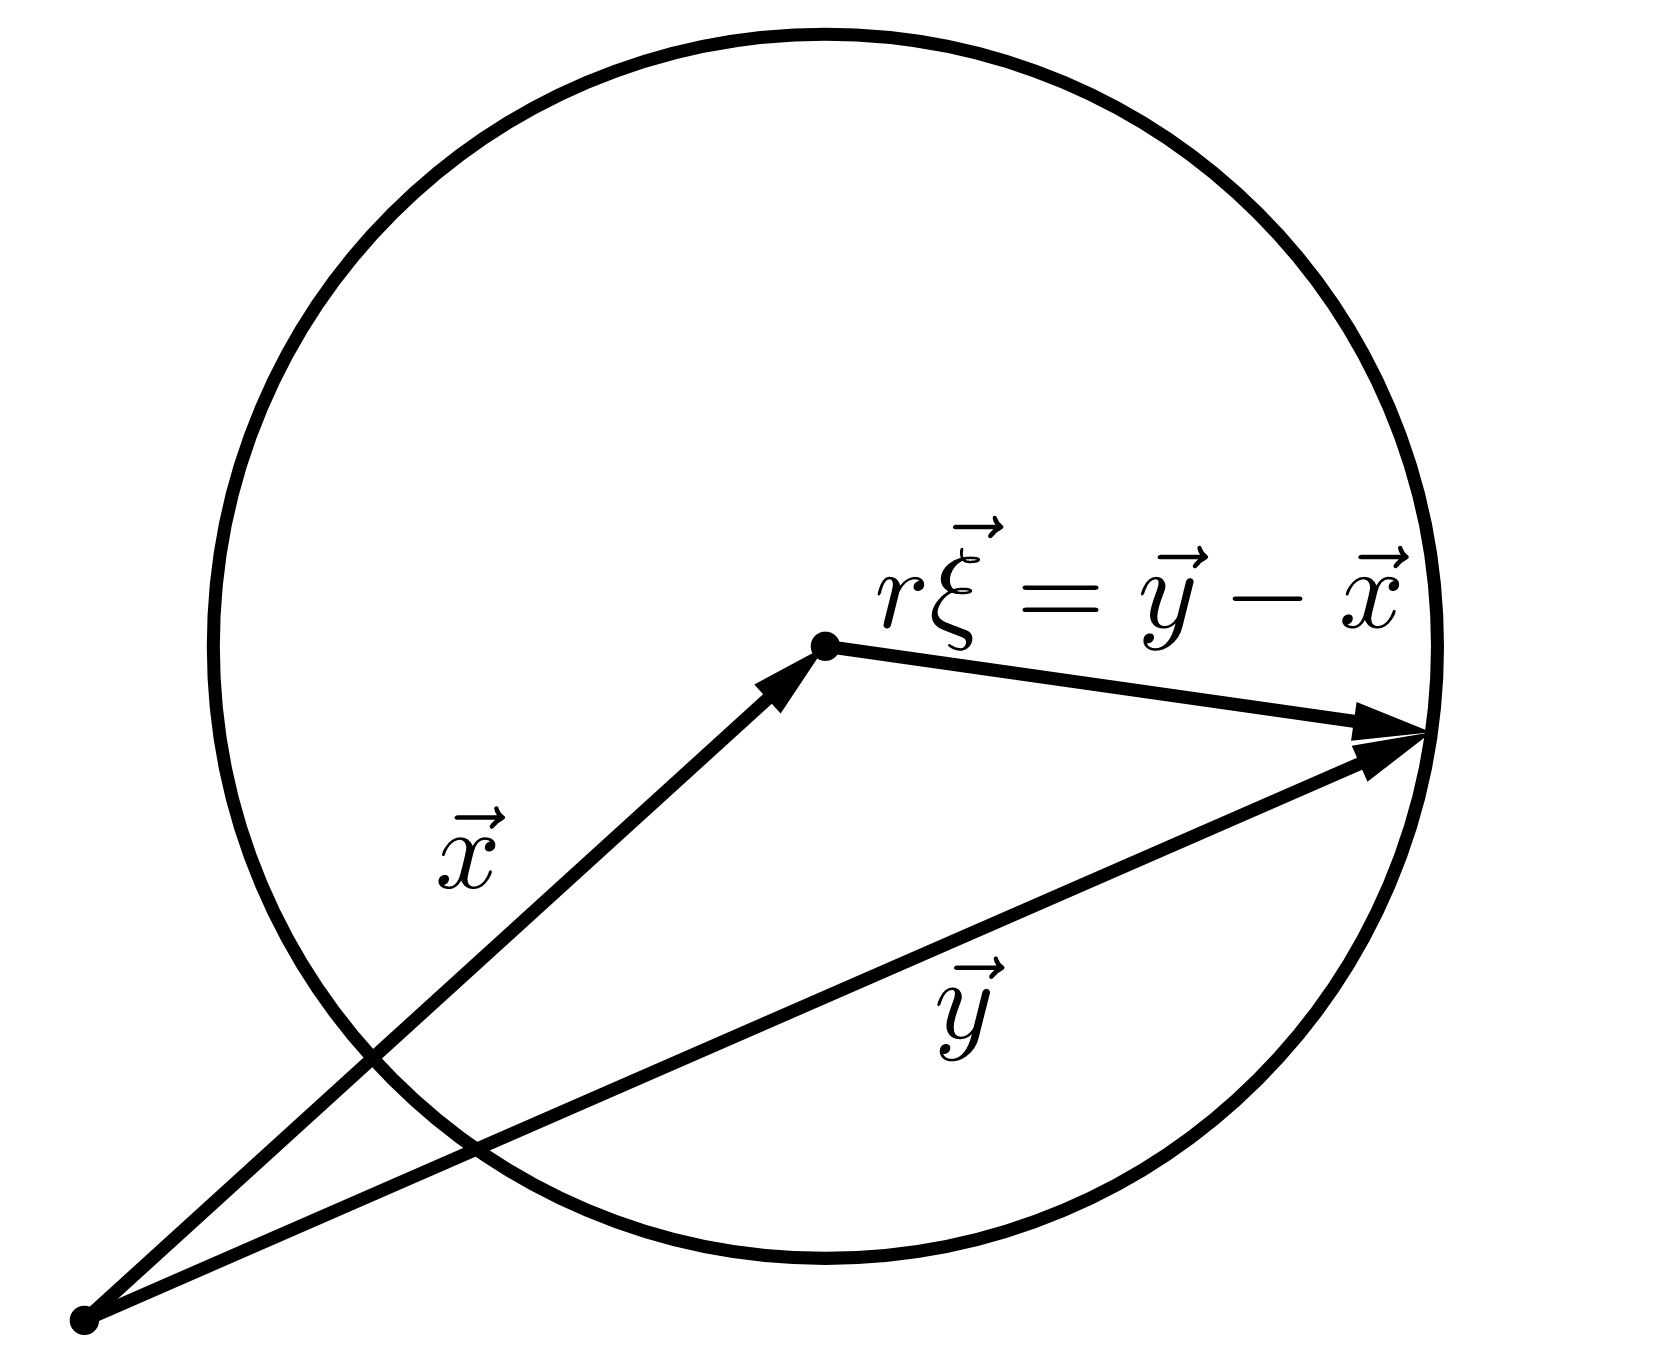
\includegraphics[scale=0.1]{xi.png}
\end{center}
\[
    y-x = \xi r    
\]
\begin{equation}
y = x + \xi r
\end{equation}
\[
    |y-x| = |\xi|r = r, \;\;\;\;\;\; |\xi| = 1    
\]
thus the surface elements are related as.
\[
    dS_y = r^{n-1} dS_\xi    
\]
substituting in (1).
\begin{equation}
M_{f}(x,r) = \frac{1}{\omega_{n}} \int_{|\xi|=1} f(x+\xi r)dS_\xi
\end{equation} 
at $r = 0$. 
\begin{equation}
M_{f}(x,0) = \frac{f(x)}{\omega_{n}} \int_{|\xi|=1} dS_\xi = f(x)
\end{equation}
the integral $\displaystyle \int_{|\xi|=1} dS_\xi$ is the surface area of a unit sphere in n dimensions which is equal to $\omega_n$

from (3) and remembering that $y$, $x$, and $\xi$ are all vectors, then we can write their components as.
\[
    y_i = x_i + \xi_i r    
\]
using this vector notation to differentiate (4) with respect to r.
\begin{align*}
\frac{\partial M_f (x,r)}{\partial r} &= \frac{1}{\omega_n} \int_{|\xi|=1} \frac{\partial f(y)}{\partial r}dS_\xi
\\
&= \frac{1}{\omega_n} \int_{|\xi|=1} \sum_{i=1}^{n} \frac{\partial f(y)}{\partial y_i}\frac{\partial y_i}{\partial r} dS_\xi
\\
&= \frac{1}{\omega_n} \int_{|\xi|=1} \sum_{i=1}^{n} \frac{\partial f(y)}{\partial y_i}\xi_i dS_\xi
\end{align*}
using the chain rule we find.$\displaystyle \frac{\partial f(y)}{\partial y_i} \frac{\partial x_i}{\partial x_i} = \frac{\partial f(y)}{\partial y_i} \frac{\partial y_i}{\partial x_i}\frac{\partial x_i}{\partial y_i} = \frac{\partial f(y)}{\partial x_i}$, since $\displaystyle \frac{\partial x_i}{\partial y_i} = 1$
\[
    \frac{\partial M_f (x,r)}{\partial r} = \frac{1}{\omega_n} \int_{|\xi|=1} \sum_{i=1}^{n} \frac{\partial f(y)}{\partial x_i}\xi_i dS_\xi    
\]
using the chain rule one more time.$\displaystyle \frac{\partial f(y)}{\partial x_i} \frac{\partial \xi_i}{\partial \xi_i}= \frac{\partial f(y)}{\partial x_i}\frac{\partial x_i}{\partial \xi_i}\frac{\partial \xi_i}{\partial x_i} = \frac{\partial f(y)}{\partial \xi_i}\frac{1}{r}$, since $\displaystyle \frac{\partial \xi_i}{\partial x_i} = \frac{1}{r}$
\begin{equation}
\frac{\partial M_f (x,r)}{\partial r} = \frac{1}{\omega_n r} \int_{|\xi|=1} \sum_{i=1}^{n} \frac{\partial f(y)}{\partial \xi_i}\xi_i dS_\xi
\end{equation}
\begin{theorem}[Divergence Theorem]
    Also called Green-Gauss-Ostrogradsky theorem relates the volume integral to the surface integral under some conditions, more precisely, the surface integral of a vector field over a closed surface (flux) is equal to the volume integral of the divergence over the region. We will use this later in our treatment.
    \[
        \int\int\int_{Volume} \frac{\partial \textbf{F}(x,y,z)}{\partial x}dV = \int\int_{Surface} \textbf{F}(x,y,z)\cos(\angle x,\vec{n}) dS    
    \]
    or in general.
    \[
        \int\int\int_{Volume} \nabla \cdot \textbf{F} dV = \int\int_{Surface} \textbf{F}\cdot \vec{n} dS
    \]
    \begin{center}
    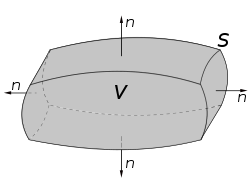
\includegraphics[scale=0.6]{div.png}
    \end{center}
\end{theorem}
comparing the form we have with the divergence theorem we see that the sum we have is the dot product of our vector function with $\xi$\footnote{the components $\xi_i$ are direction cosines, i.e $\xi_{1}^{2}+\xi_{2}^{2}+...+\xi_{n}^{2} = 1$} which is the unit vector always normal to the surface of the sphere by our definition, and we can transform our integral to a volume integral.
\[
    \frac{\partial M_f (x,r)}{\partial r} = \frac{1}{\omega_n r} \int_{|\xi|\leq 1} \sum_{i=1}^{n} \frac{\partial^2 f(y)}{\partial \xi_{i}^{2}} d\xi    
\]
using the chain rule we have.
\begin{align*}
\frac{\partial M_f (x,r)}{\partial r} &= \frac{r^2}{\omega_n r} \int_{|\xi|\leq 1} \sum_{i=1}^{n} \frac{\partial^2 f(y)}{\partial x_{i}^{2}} d\xi
\\
&=\frac{r}{\omega_n} \nabla_{x}^{2} \int_{|\xi|\leq 1} f(y)d\xi
\end{align*}
notice that .
\[
    \frac{\partial M_f (x,0)}{\partial r} = 0    
\]
now we will change our volume element from the relation (3).\footnote{remember that y is a vector thus $dy = dy_1 dy_2 dy_3 ...dy_n$ and since $dy_i = rd\xi_i$ then $dy = rrr...d\xi_1 d\xi_2 d\xi_3 ...$}
\[
    d\xi = \frac{1}{r^n}dy    
\]
thus we have 
\begin{align*}
\frac{\partial M_f (x,r)}{\partial r} &= \frac{r}{\omega_n r^n} \nabla_{x}^{2} \int_{|y-x|\leq r} f(y)dy
\\
&= \frac{1}{\omega_n r^{n-1}} \nabla_{x}^{2} \int_{|y-x|\leq r} f(y)dy
\\
&= \frac{1}{\omega_n r^{n-1}} \nabla_{x}^{2} \int_{\rho = 0}^{r} \int_{|y-x| = \rho} f(y)dS_y d\rho
\end{align*}
rearranging and multiply and divide by $\rho^{n-1}$.
\[
    r^{n-1} \frac{\partial M_f (x,r)}{\partial r} =  \nabla_{x}^{2}\int_{\rho = 0}^{r} \frac{\rho^{n-1}}{\omega_n \rho^{n-1}} \int_{|y-x|= \rho}f(y)dS_y d\rho    
\]
notice that on the right hand side an expression the same as the spherical mean (4) is attained thus we substitute .
\[
    r^{n-1} \frac{\partial M_f (x,r)}{\partial r} = \nabla_{x}^{2}\int_{\rho = 0}^{r} \rho^{n-1} M_{f}(x,r) d\rho    
\]
differentiating the expression with respect to r.
\begin{align*}
\frac{\partial}{\partial r}\left( r^{n-1} \frac{\partial M_f (x,r)}{\partial r}\right) &= \nabla_{x}^{2} \frac{\partial}{\partial r}\int_{\rho = 0}^{r} \rho^{n-1} M_{f}(x,r) d\rho
\\
r^{n-1} \frac{\partial^2 M_f (x,r)}{\partial r^2} + (n-1)r^{n-2}r^{n-1} \frac{\partial M_f (x,r)}{\partial r} &= \nabla_{x}^{2} r^{n-1} M_f (x,r)
\end{align*}
rearranging and simplifying we finally arrive at Darboux's equation (2) where $ V=M_f (x,r) $.
\[
    \frac{\partial^2 M_f (x,r)}{\partial r^2} + \frac{n-1}{r} \frac{\partial M_f (x,r)}{\partial r} = \nabla_{x}^{2} M_f (x,r)    
\]

\begin{figure*}[b]
    \begin{enrichment}{Jean Gaston Darboux}{Darboux.jpg}{2.4}{.8}{.17}
        Born in Nimes Jean Gaston Darboux (1842-1917) was a renowned 
        French mathematician who made significant contributions to Partial Differential Equations (PDEs). 
        Darboux's work centered on the theory of linear and nonlinear partial differential equations, 
        which are fundamental to understanding various physical phenomena and mathematical models. 
        He tackled important questions related to the existence, uniqueness, and regularity of solutions to these equations, 
        laying the groundwork for future investigations in the field.
    \end{enrichment}    
\end{figure*}

\newpage

\setcounter{equation}{0}
\setcounter{footnote}{0}
\subsection{Kirchhoff's Formula}
We have seen how formula d'Almbert can solve the one dimensional wave equation Cauchy problem but the solution of the wave equation in dimensions higher than one shows to be more complicated. 
Our attempt to solve the three dimensional wave equation 
we will use the results of the spherical mean and Darboux's equation to develop an effective formula to solve three dimensional wave equation Cauchy problems called Kircchoff's formula.
\par
Consider the following three dimensional wave equation Cauchy problem.
\begin{equation}
\frac{\partial^2 u(x,t)}{\partial t^2} = c^2 \nabla_{x}^{2}u(x,t), \;\;\;\;\;\; c\neq 0 ,\;\;\; t > 0
\end{equation}
\begin{equation}
    \text{I.C} \quad \Longrightarrow \quad 
    \begin{cases}
    u\left(x,0 \right) = \phi\left(x\right)
    \\
    \\
    \displaystyle \frac{\partial u\left(x,0 \right)}{\partial t} = \psi\left(x\right)
    \end{cases}
\end{equation}
where $x = (x_1,x_2,x_3)$ is a three dimensional vector.
\par
we start by considering Darboux's equation (54) in n = 3.
\begin{align}
\frac{\partial^2 M_f (x,r)}{\partial r^2} + \frac{2}{r} \frac{\partial M_f (x,r)}{\partial r} &= \nabla_{x}^{2} M_f (x,r) \notag
\\ 
r\frac{\partial^2 M_f (x,r)}{\partial r^2} + 2 \frac{\partial M_f (x,r)}{\partial r} &= r\nabla_{x}^{2} M_f (x,r)
\end{align}
we notice that.
\begin{align*}
\frac{\partial }{\partial r}\left(rM_f (x,r) \right) &= r\frac{\partial M_f(x,r)}{\partial r} +M_f (x,r)
\\
\frac{\partial^2 }{\partial r^2}\left(rM_f (x,r) \right) &= r\frac{\partial^2 M_f(x,r)}{\partial r^2} + \frac{\partial M_f(x,r)}{\partial r}  + \frac{\partial M_f(x,r)}{\partial r}
\end{align*}
\begin{equation}
\frac{\partial^2 }{\partial r^2}\left(rM_f (x,r) \right) = r\frac{\partial^2 M_f(x,r)}{\partial r^2} + 2\frac{\partial M_f(x,r)}{\partial r}
\end{equation}
substituting (4) in (3).
\begin{equation}
\frac{\partial^2 }{\partial r^2}\left(rM_f (x,r) \right) = r\nabla_{x}^{2} M_f (x,r)
\end{equation}
we now consider the spherical mean of the function $u$ where n = 3.\footnote{when n = 3 then $\omega_3 = 4\pi$ the surface area of a 3d sphere}
\[
    M_{u}(x,t,r) = \frac{1}{4\pi r^2} \int_{|y-x|=r} f(y)dS_y    
\]
calculating the spherical mean of the whole equation (1) we get.
\[
    \frac{\partial^2}{\partial t^2} M_{u}(x,t,r) = c^2 \nabla_{x}^{2}M_{u}(x,t,r)    
\]
multiply by r.
\[
    \frac{\partial^2}{\partial t^2} r M_{u}(x,t,r) = c^2 r\nabla_{x}^{2}M_{u}(x,t,r)    
\]
from (5) we get.
\begin{equation}
    \frac{\partial^2}{\partial t^2} \left[r M_u (x,t,r) \right] = c^2 \frac{\partial^2 }{\partial r^2}\left[r M_u (x,t,r) \right]    
\end{equation}

\newpage 

the initial conditions will be.
\begin{equation}
rM_{u}(x,0,r) = rM_\phi(x,r) = \frac{r}{4\pi r^2} \int_{|y-x|=r}\phi(y)dS_y
\end{equation}
\begin{equation}
\frac{\partial}{\partial t}\left(rM_{u}(x,0,r)\right) = rM_\psi(x,r) = \frac{r}{4\pi r^2} \int_{|y-x|=r}\psi(y)dS_y
\end{equation}
we notice that this is a one dimensional wave equation that can be solved using the method developed earlier d'Alembert formula.
\[
    rM_u(x,t,r) = \frac{1}{2}\left[(r+ct)M_\phi(x,r+ct)+(r-ct)M_\phi(x,r-ct)\right]+\frac{1}{2c}\int_{x-ct}^{x+ct} sM_\psi(x,s)ds    
\]
\begin{equation}
M_u(x,t,r) = \frac{1}{2r}\left[(r+ct)M_\phi(x,r+ct)+(r-ct)M_\phi(x,r-ct)\right]+\frac{1}{2cr}\int_{x-ct}^{x+ct} sM_\psi(x,s)ds
\end{equation}
we note that.
\[
\lim_{r\to 0} M_u(x,t,r) = u(x,t)    
\]
now we start studying the limit to find our target function $u(x,t)$.
\begin{align}
\lim_{r\to 0} M_u(x,t,r) = \lim_{r\to 0}\frac{1}{2r}\left[(r+ct)M_\phi(x,r+ct)+(r-ct)M_\phi(x,r-ct)\right] \notag
\\
+\lim_{r\to 0}\frac{1}{2cr}\int_{r-ct}^{r+ct} sM_\psi(x,s)ds
\end{align}
the first limit can be rearranged to.
\[
    \lim_{r\to 0} \frac{1}{2r}\left[rM_\phi(x,r+ct)+ctM_\phi(x,r+ct)+rM_\phi(x,r-ct)-ctM_\phi(x,r-ct)\right]    
\]
rearranging one more time and noting that the spherical mean function is an even function $\displaystyle M_f(r)=M_f(-r)$ thus we can multiply the r variable by negative one.
\begin{align*}
    \lim_{r\to 0} \frac{1}{2r}\left[rM_\phi(x,r+ct)+rM_\phi(x,r-ct)\right] & +\lim_{r\to 0} \frac{1}{2r}ct\left[M_\phi(x,r+ct)-M_\phi(x,ct-r)\right]
    \\
    \frac{1}{2} \lim_{r\to 0} \left[M_\phi(x,r+ct)+M_\phi(x,r-ct)\right] & + ct \lim_{r\to 0} \frac{\left[M_\phi(x,r+ct)-M_\phi(x,ct-r)\right]}{2r}
    \\
    \frac{1}{2} \left[M_\phi(x,ct)+M_\phi(x,-ct)\right] & + ct \frac{\partial M_\phi(x,ct)}{\partial ct}
\end{align*}
the first limit is equal to $M_\phi(x,ct)$ due to the function being even and we notice that the second limit is the definition of the derivative$\displaystyle f'(x) = \lim_{h\to 0} \frac{f(x+h) - f(x-h)}{2h}$ with respect to $ct$ thus the limit is finally evaluated to.
\[
    \lim_{r\to 0}\frac{1}{2r}\left[(r+ct)M_\phi(x,r+ct)+(r-ct)M_\phi(x,r-ct)\right] = M_\phi(x,ct) + ct\frac{\partial}{\partial ct}(M_\phi(x,ct))    
\]
consider .
\[
    \frac{\partial}{\partial t}[tM_\phi(x,ct)] = M_\phi(x,ct)+t \frac{\partial M_\phi(x,ct)}{\partial ct}\frac{\partial ct}{\partial t} = M_\phi(x,ct)+ct \frac{\partial M_\phi(x,ct)}{\partial ct}    
\]
\[
\therefore \lim_{r\to 0}\frac{1}{2r}\left[(r+ct)M_\phi(x,r+ct)+(r-ct)M_\phi(x,r-ct)\right] = \frac{\partial}{\partial t}[tM_\phi(x,ct)]    
\]
now considering the second limit.
\[
    \lim_{r\to 0}\frac{1}{2cr}\int_{r-ct}^{r+ct} sM_\psi(x,s)ds    
\]
direct substitution will result in an undetermined form $\frac{0}{0}$ since the function inside the integral is an odd function thus the symmetrical integral will vanish thus we will utilize l'Hopital's rule to find the limit.
\begin{enrichment*}{l'Hopital's rule}
    \[
        \lim_{{x \to c}} \frac{{f(x)}}{{g(x)}} = \lim_{{x \to c}} \frac{{f'(x)}}{{g'(x)}}    
    \]
\end{enrichment*}
\[
    \lim_{r\to 0}\frac{1}{2cr}\int_{r-ct}^{r+ct} sM_\psi(x,s)ds = \lim_{r\to 0}\frac{1}{2c}\frac{\partial}{\partial r}\left[\int_{r-ct}^{r+ct} sM_\psi(x,s)ds\right]    
\]
to find the derivative of the integral we use Libenz rule.
\begin{enrichment*}{Libenz rule}
    \[
        \frac{d}{dx}\int_{a(x)}^{b(x)} f(x,y)dy = \frac{db(x)}{dx}f(x,b(x))-\frac{da(x)}{dx}f(x,a(x)) + \int_{a(x)}^{b(x)} \frac{\partial f(x,y)}{\partial x} dy    
    \]
\end{enrichment*}
in our case
\begin{align*}
\frac{\partial}{\partial r}\left[\int_{r-ct}^{r+ct} sM_\psi(x,s)ds\right] &= (r+ct)M_\psi(x,r+ct) - (r-ct)M_\psi(x,r-ct) + \int_{r-ct}^{r+ct} \frac{\partial}{\partial r} sM_\psi(x,s)ds
\\
 &= ct[M_\psi(x,r+ct)+M_\psi(x,r-ct)]
\end{align*}
\\
thus the limit will become.
\[
    \lim_{r\to 0}\frac{1}{2cr}\int_{r-ct}^{r+ct} sM_\psi(x,s)ds = \lim_{r\to 0}\frac{ct[M_\psi(x,r+ct)+M_\psi(x,r-ct)]}{2c}    
\]
which is finally evaluated to.
\[
    \lim_{r\to 0}\frac{1}{2cr}\int_{r-ct}^{r+ct} sM_\psi(x,s)ds = tM_\psi(x,ct)    
\]
we now finally substitute the first and the second limit in (10).
\[
    u(x,t) = \lim_{r\to 0} M_u(x,t,r) = \frac{\partial}{\partial t}[tM_\phi(x,ct)] + tM_\psi(x,ct)    
\]
using the definition of spherical mean with $r=ct$ our final formula becomes.
\begin{figure*}[b]
    \begin{enrichment}{Gustav Kirchhoff}{Kirchhoff.jpg}{2.4}{.8}{.17}
        Gustav Kirchhoff (1824-1887) was a prominent German physicist
        Kirchhoff made significant advancements in the understanding of wave phenomena and the mathematical modeling of physical systems using PDEs.
        One of Kirchhoff's most notable contributions in PDEs is his formulation of the Kirchhoff equations, which describe the propagation of waves in elastic materials, such as solids and thin plates. These equations are fundamental to the study of vibrations, acoustics, and the behavior of mechanical systems subjected to dynamic loads.
    \end{enrichment}    
\end{figure*}
\[
    u(x,t) = \frac{\partial}{\partial t}\left[\frac{1}{4\pi c^2 t}\int_{|y-x|=ct}\phi(y)dS_y\right] + \frac{1}{4\pi c^2 t}\int_{|y-x|=ct}\psi(y)dS_y    
\]
which is called Kirchhoff's Formula.


\section{Laplace's Equation}
Laplace's equation is one of the most important PDE in mathematical physics most notably in the study of electromagnetism. Our first stem is get accustomed to some terminology. Consider the following problem.
\[
    \nabla^2 u(x,y)= \frac{\partial^2 u(x,y,z)}{\partial x^2}+\frac{\partial^2 u(x,y,z)}{\partial y^2} = 0 \;\;\;\; , (x,y) \in G    
\]
where G is a simply bounded connected domain whose boundary $\gamma$ is a contour.
\\
the boundary condition for this problem is.
\[
    u(x,y)|_\gamma = f(x,y)    
\]
\begin{center}
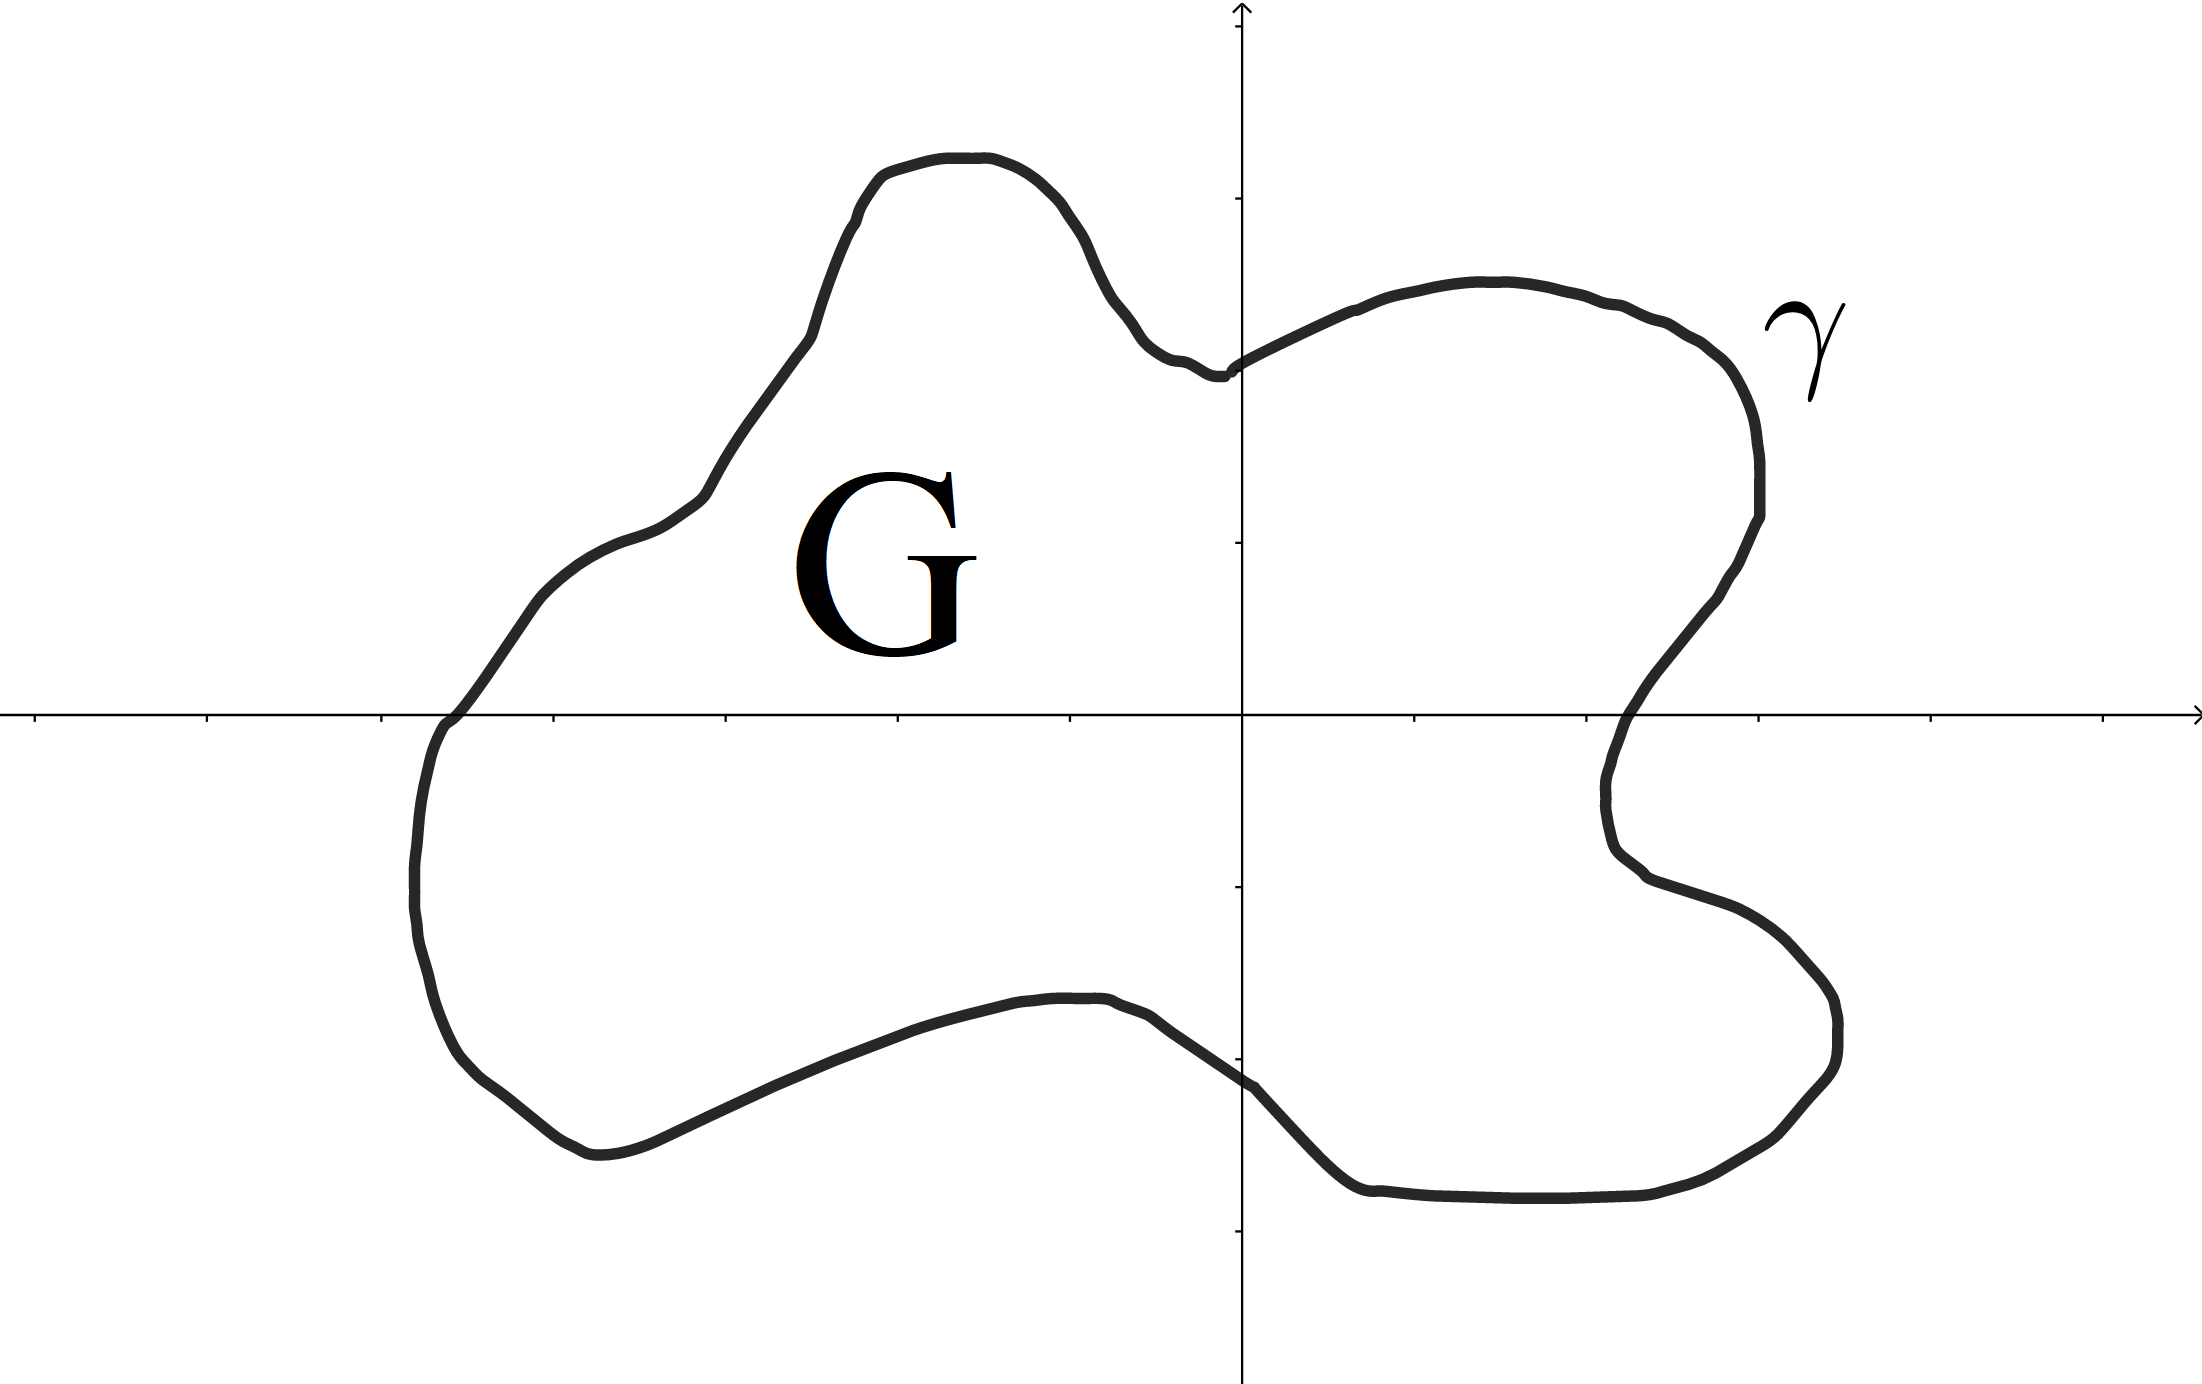
\includegraphics[scale=0.1]{domain.png}
\end{center}
we can see that this is a Dirichlet problem.
\par
if the function $u$ that satisfy the Laplace equation and is in the set of two dimensional continuous functions on the domain G $u \in C^2(G)$, 
i.e. all of $u, \frac{\partial u}{\partial x}, \frac{\partial u}{\partial y}, \frac{\partial^2 u}{\partial x^2},\frac{\partial^2 u}{\partial y^2}$,
are continuous functions on G, then the function $u$ is called a harmonic function on G.

\setcounter{equation}{0}
\subsection{Solution of Laplace's Equation on a Circle}

consider the partial differential equation
\begin{equation}
\nabla^2 u(x,y) = \frac{\partial^2 u(x,y)}{\partial x^2} + \frac{\partial^2 u(x,y)}{\partial y^2} = 0\;, \;\;\; \forall (x,y) \in G
\end{equation}
\begin{equation}
\text{I.C} \quad \Longrightarrow \quad u(x,y)|_\gamma = f(x,y)
\end{equation}

\begin{center}
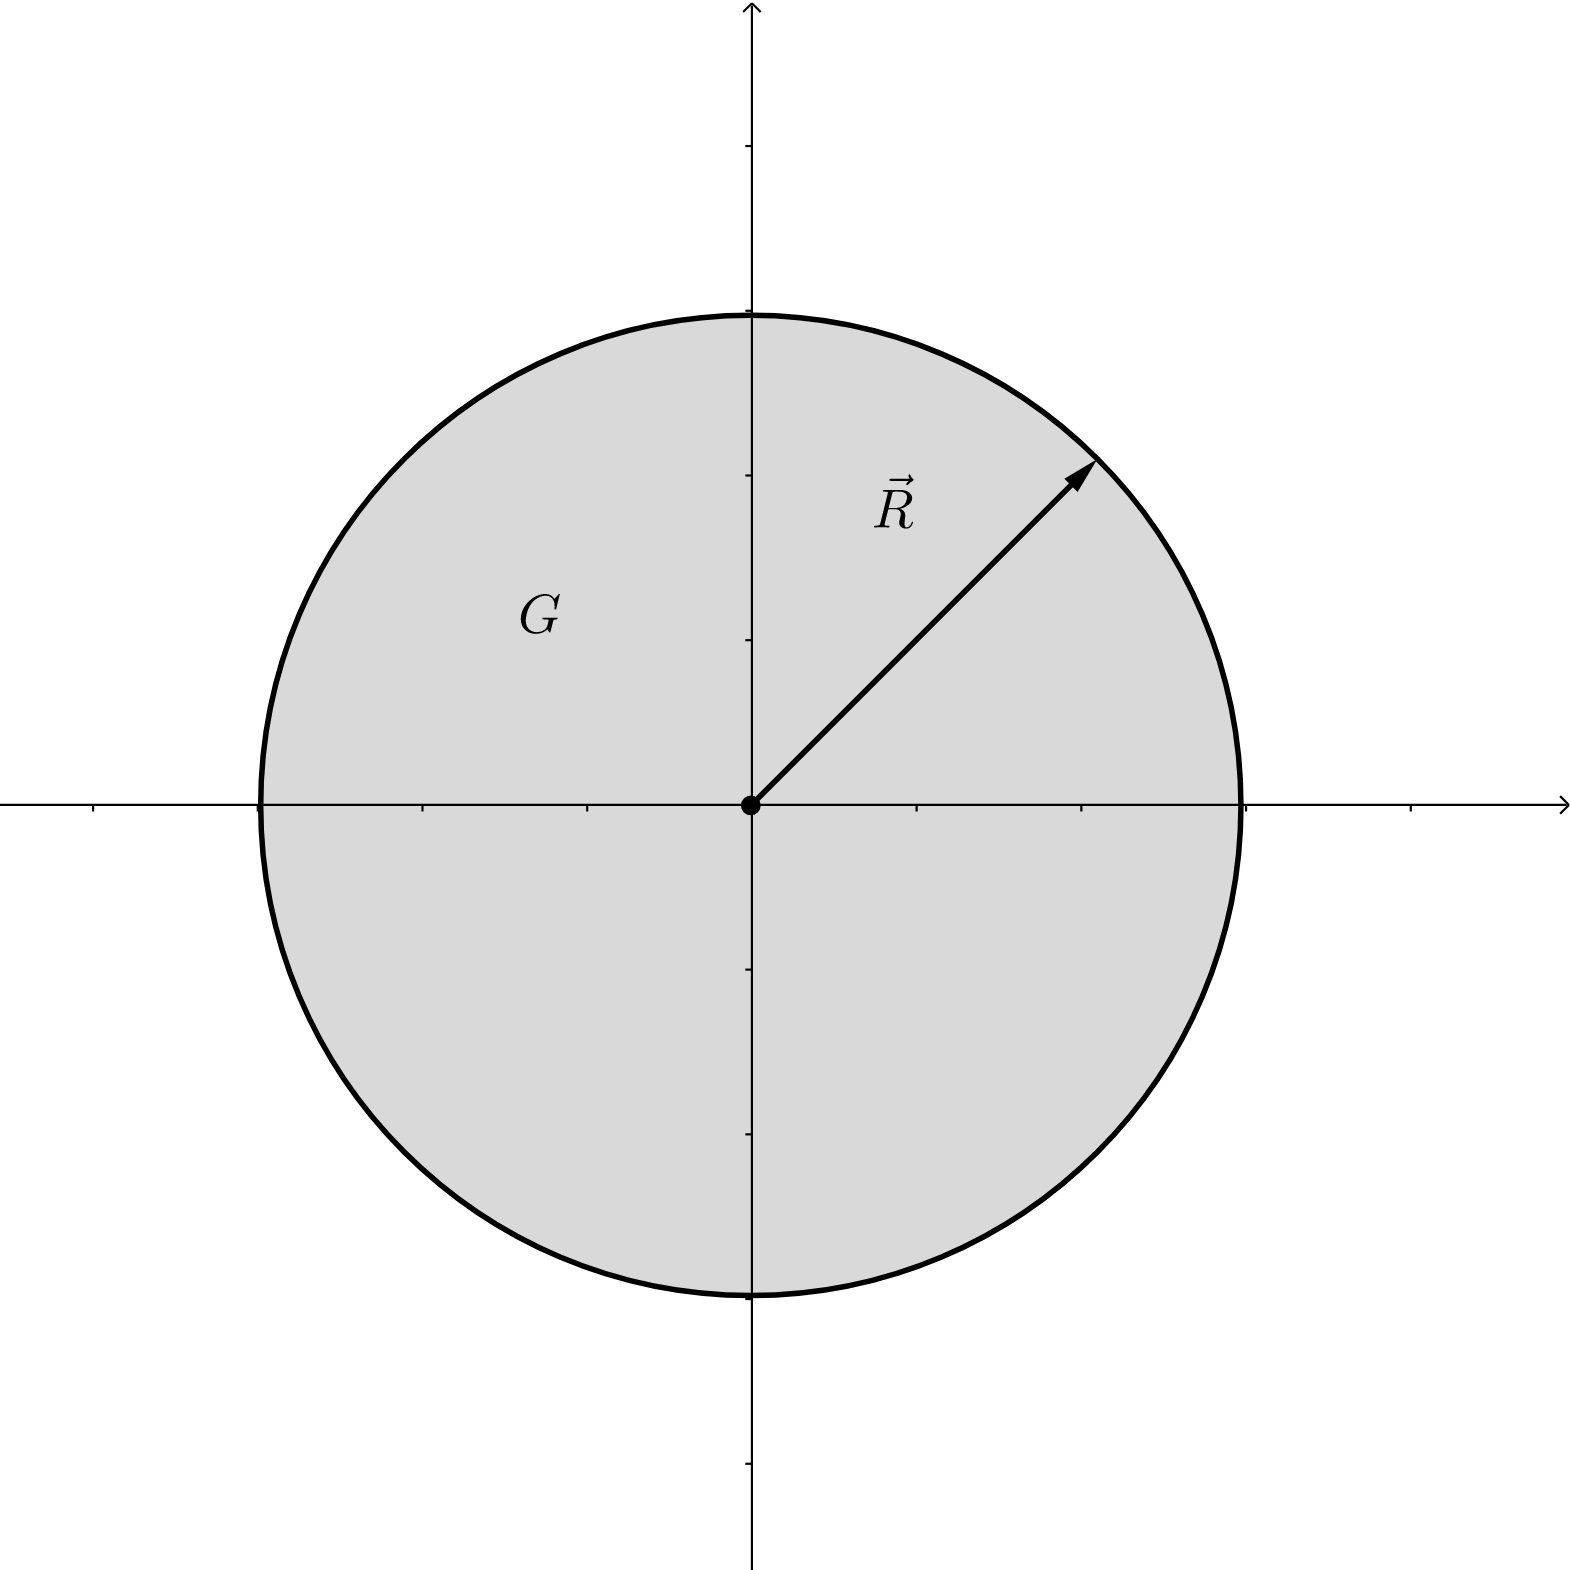
\includegraphics[scale=0.17]{circle.png}
\end{center}
\begin{align*}
G &= \left\lbrace (x,y):x^2+y^2 < R^2 \right\rbrace
\\
\gamma &= \left\lbrace (x,y):x^2+y^2 = R^2 \right\rbrace
\end{align*}
buy puting $x = r cos(\theta)$ and $y = r sin(\theta)$ and recreate equation (1) using chain rule we can express (1) as.
\begin{equation}
r^2 \frac{\partial^2 u(r,\theta)}{\partial r^2} + r \frac{\partial u(r,\theta)}{\partial r} + \frac{\partial^2 u(r,\theta)}{\partial \theta^2} = 0
\end{equation}
notice from (3) that the derivatives of $r$ and $\theta$ can be separated thus utilizing the separation of variables method.
\begin{align*}
u(r,\theta) &= V(r)F(\theta)
\\
\frac{\partial u}{\partial r} &= \frac{d V(r)}{dr}F(\theta)
\\
\frac{\partial^2 u}{\partial r^2} &= \frac{d^2 V(r)}{dr^2}F(\theta)
\\
\frac{\partial^2 u}{\partial \theta^2} &= V(r)\frac{d^2 F(\theta)}{d\theta^2}
\end{align*}
therefore we get.
\begin{equation}
r^2F(\theta)\frac{d^2 V(r)}{dr^2} +rF(\theta)\frac{d V(r)}{dr} + V(r)\frac{d^2 F(\theta)}{d\theta^2} = 0
\end{equation}
dividing (4) by $V(r)F(\theta)$ we get.
\begin{equation}
\frac{r^2}{V(r)}\frac{d^2 V(r)}{dr^2} +\frac{r}{V(r)}\frac{d V(r)}{dr} + \frac{1}{F(\theta)}\frac{d^2 F(\theta)}{d\theta^2} = 0
\end{equation}
\[
    \frac{r^2}{V(r)}\frac{d^2 V(r)}{dr^2} +\frac{r}{V(r)}\frac{d V(r)}{dr} = n^2 = -\frac{1}{F(\theta)}\frac{d^2 F(\theta)}{d\theta^2}    
\]
we start solving for the $F(\theta)$. 
\[
    \frac{d^2 F(\theta)}{d\theta^2} = -n^2F(\theta)    
\]
the solution will be. 
\begin{equation}
F(\theta) = A\;\cos(n\theta)+B\;\sin(n\theta)
\end{equation}
then solving for $V(r)$.
\[
r^2\frac{d^2 V(r)}{dr^2} +r\frac{d V(r)}{dr} = n^2V(r)    
\]
by puting $r = e^t$
\begin{align*}
\frac{dV(r)}{dr} &= \frac{dV(r)}{dt}\frac{dt}{dr} = e^{-t} \frac{dV(r)}{dt}\;\Rightarrow  r \frac{dV(r)}{dr}=\frac{dV(r)}{dt}
\\
\frac{d^2V(r)}{dr^2} &= \frac{d}{dr}\left[e^{-t} \frac{dV(r)}{dt}\right]
\\
&=  \frac{d}{dt}\left[e^{-t} \frac{dV(r)}{dt}\right] \frac{dt}{dr} 
\\
&= \frac{d}{dt}\left[e^{-t} \frac{dV(r)}{dt}\right] e^{-t}
\\
&= e^{-2t}\left[-\frac{dV(r)}{dt}+\frac{d^2V(r)}{dt^2}\right] \;\Rightarrow\; r^2\frac{d^2V(r)}{dr^2} = \frac{d^2V(r)}{dt^2}-\frac{dV(r)}{dt}
\end{align*}
substituting will result in.
\begin{align*}
\frac{d^2V(r)}{dt^2}-\frac{dV(r)}{dt}+\frac{dV(r)}{dt}&=n^2V(r)
\\
\frac{d^2V(r)}{dt^2} &= n^2V(r)
\end{align*}
\[
\therefore V(r) = Ce^{nt}+De^{-nt} = Cr^n+Dr^{-n}    
\]
to maintain the continuity of the function we put D=0.
\[
\therefore V(r) = Cr^n
\]
substituting V and F in u.
\begin{equation}
u(r,\theta) = r^n[A\;cos(n\theta)+B\;sin(n\theta)]
\end{equation}
from this the boundary condition becomes a function only in $\theta$.
\begin{equation}
u|_\gamma = H(\theta)
\end{equation}
taking the sum of all solutions we get.
\[
    u(r,\theta) = a_o + \sum_{n=1}^{\infty} r^n[a_n\;cos(n\theta)+b_n\;sin(n\theta)]    
\]
at $\gamma \longrightarrow $ r = 1.
\[
    H(\theta) = a_o + \sum_{n=1}^{\infty} a_n\;cos(n\theta)+b_n\;sin(n\theta) 
\]
then we find the Fourier coefficients.
\begin{align*}
a_o &= \frac{1}{2\pi}\int_{0}^{2\pi} H(\psi ) d\psi 
\\
a_n &=\frac{1}{\pi}\int_{0}^{2\pi} H(\psi ) cos(n\psi ) d\psi 
\\
a_n &=\frac{1}{\pi}\int_{0}^{2\pi} H(\psi ) \sin(n\psi ) d\psi 
\end{align*}
then we get.
\begin{align*}
u(r,\theta) &= \frac{1}{2\pi}\int_{0}^{2\pi} H(\psi ) d\psi  + \frac{1}{\pi}\sum_{n=1}^{\infty} r^n \int_{0}^{2\pi} H(\psi )[\cos(n\psi )\cos(n\theta) + \sin(n\psi )\sin(n\theta)]d\psi 
\\
u(r,\theta) &= \frac{1}{2\pi}\int_{0}^{2\pi} H(\psi ) d\psi  + \frac{1}{\pi}\sum_{n=1}^{\infty}r^n\int_{0}^{2\pi} H(\psi )\cos[n(\psi  - \theta)]d\psi 
\end{align*}
\begin{enrichment*}{}
    $\cos[A-B] = \cos(A)\cos(B) + \sin(A)\sin(B)$
\end{enrichment*}
from the value of the exponential series we can get.
\[
    S_1 = \sum_{n=1}^{\infty} r^n \cos(n\phi),\;\;\; S_2 =\sum_{n=1}^{\infty}r^n \sin(n\phi), \;\;\; \phi = \psi  - \theta    
\]
\[
    S_1 + i S_2 = \sum_{n=0}^{\infty} r^n e^{in\phi}    
\]
this is the form of a geometric series the value of the summition is
\[
    \sum_{n=0}^{\infty} r^n e^{in\phi} = \frac{r e^{i\phi}}{1- r e^{i\phi}}
\]
we now manipulate the expression to obtain the real part.
\\
\begin{align*}
\frac{r^n e^{i\phi}}{1- r^n e^{i\phi}} &= \frac{r(cos\phi+isin\phi)}{1-r(cos\phi+isin\phi)}
\\
&= \frac{r(cos\phi+isin\phi)}{(1-rcos\phi)-irsin\phi} \cdot \frac{(1-rcos\phi)+irsin\phi}{(1-rcos\phi)+irsin\phi}
\\
&= \frac{rcos\phi - r^2 + ir \sin\phi}{1-2rcos\phi+r^2}
\\
&= \frac{rcos\phi - r^2}{1-2rcos\phi+r^2} + i \frac{\sin\phi}{1-2rcos\phi+r^2}
\end{align*}
we find that.
\[
    S_1 = \frac{rcos\phi - r^2}{1-2rcos\phi+r^2}    
\]
substituting in the expression for u we get.
\begin{align*}
u(r,\theta) &= \frac{1}{2\pi}\int_{0}^{2\pi} H(\psi ) d\psi  + \frac{1}{\pi}\int_{0}^{2\pi} H(\psi )\frac{rcos(\psi  -\theta) - r^2}{1-2rcos(\psi  -\theta)+r^2}d\psi 
\\
            &= \frac{1}{2\pi}\int_{0}^{2\pi} H(\psi )\frac{2rcos(\psi  -\theta) - 2r^2+1-2rcos(\psi  -\theta)+r^2}{1-2rcos(\psi  -\theta)+r^2}d\psi 
\end{align*}
simplify.
\[
    u(r,\theta) = \frac{1}{2\pi}\int_{0}^{2\pi} H(\psi )\frac{1-r^2}{1-2rcos(\psi  -\theta)+r^2}d\psi     
\]
and for a circle of radius R we get Poisson's Formula.
\[
    u(r,\theta) = \frac{1}{2\pi R}\int_{0}^{2\pi R} H(\beta)\frac{R^2-r^2}{R^2-2Rrcos(\psi  -\theta)+r^2}d\beta \;\;\;, \;\;\;\; \beta = R\psi     
\]
we can easily find u in terms of x and y, the two forms are equivalent.

\subsection{Harmonic Functions}
we will discuss some properties or theorems of the harmonic function

\begin{observation}
    u(x,y) at the center of the circle where r=0 that is when x=0 and y=0 is
    \[
        u(0,0) = \frac{1}{2\pi R}\int_{0}^{2\pi R} H(\beta)\frac{R^2-(0)^2}{R^2-2R(0)cos(\psi  -\theta)+(0)^2}d\beta =\frac{1}{2\pi R}\int_{0}^{2\pi R} H(\beta)d\beta     
    \]
\end{observation}    

\begin{theorem}[Liouville Theorem]
    A harmonic function of the whole plane, i.e. $(x,y) \in \mathbb{R}^2$, can not be bounded from above or bounded from below unless it is constant.    
\end{theorem}
\begin{proof}
    assume the harmonic function is bounded from below, i.e.    
    \[
        u(x,y) \geq m \;\; \forall (x,y) \in \mathbb{R}^2     
    \]
    without loss of generality $m > 0$ is assumed.
    \\
    we know that $ -1 \leq cos(\theta) \leq 1$
    \begin{align*}
        \therefore
        \frac{R^2-r^2}{R^2+2Rr+r^2} &\leq \frac{R^2-r^2}{R^2-2Rrcos(\psi  -\theta)+r^2} \leq \frac{R^2-r^2}{R^2-2Rr+r^2}
        \\
        \frac{(R-r)(R+r)}{{(R+r)}^2} &\leq \frac{R^2-r^2}{R^2-2Rrcos(\psi  -\theta)+r^2} \leq \frac{(R-r)(R+r)}{{(R-r)}^2}
        \\
        \frac{R-r}{R+r} &\leq \frac{R^2-r^2}{R^2-2Rrcos(\psi  -\theta)+r^2} \leq \frac{R+r}{R-r}
    \end{align*}
    therefore
    \[
        \frac{1}{2\pi R}\int_{0}^{2\pi R} H(\beta)\frac{R-r}{R+r} d\beta \leq \frac{1}{2\pi R}\int_{0}^{2\pi R} H(\beta)\frac{R^2-(0)^2}{R^2-2R(0)cos(\psi  -\theta)+(0)^2}d\beta \leq \frac{1}{2\pi R}\int_{0}^{2\pi R} H(\beta)\frac{R+r}{R-r} d\beta    
    \]
    and from observation 5.1 
    \[
        \frac{R-r}{R+r} u(0,0) \leq u(x,y) \leq \frac{R+r}{R-r} u(0,0)    
    \]
    taking the limit as $R \to \infty$ to include the whole plane we get.
    \[
        u(0,0) \leq u(x,y) \leq u(0,0) \;\;\; \Rightarrow \;\;\; u(x,y) = u(0,0)    
    \]
    therefore the function is constant when it is bounded from below, the same argument can be used for bounded from above case.
\end{proof}

\begin{theorem}[Regularity Theorem]
    If u is a harmonic and continuous function on G and its boundary $\gamma$, then u is analytic at every point on G, i.e. can be represented as as a power series and can be differentiated infinite times.    
\end{theorem}
\begin{proof}
    we know that.       
    \[
        u(x,y) = \frac{a_o}{2} + \sum_{n=1}^{\infty} r^n[a_n\;\cos(n\theta)+b_n\;\sin(n\theta)]    
    \]
    and we know from de Moivre's formula that.
    \[
        \cos(n\theta) = \sum_{k=0}^{n} A_k {(\cos\theta)}^k {(\sin\theta)}^{n-k}    
    \]
    and
    \[
        \sin(n\theta) =  \sum_{k=0}^{n} B_k {(\cos\theta)}^k {(\sin\theta)}^{n-k}    
    \]
    substituting in $u(x,y)$ we get.
    \[
        u(x,y) = \frac{a_o}{2} + \sum_{n=1}^{\infty} r^n\left[a_n\sum_{k=0}^{n} A_k (cos\theta)^k (sin\theta)^{n-k}\right] + \sum_{n=1}^{\infty} r^n\left[b_n\sum_{k=0}^{n} B_k (cos\theta)^k (sin\theta)^{n-k}\right]    
    \]
    put $r^n = r^{n-k}r^k $ and we know that $x = rcos\theta$ and $y=rsin\theta$.
    \[
        u(x,y) = \frac{a_o}{2} + \sum_{n=1}^{\infty}\sum_{k=0}^{n} a_n A_k x^k y^{n-k} + \sum_{n=1}^{\infty}\sum_{k=0}^{n}b_n B_k x^k y^{n-k}    
    \]
    \[
        u(x,y) = \frac{a_o}{2} + \sum_{n=1}^{\infty}\sum_{k=0}^{n} C_{n,k} x^k y^{n-k}
    \]
    therefore the function can be represented as a power series at any point, i.e. is analytical.
\end{proof}
\begin{figure*}[b]
\begin{enrichment*}{Analytic Function}
    is a Function that can be represented by a convergent power series in a region around each point within its domain. It is a function that is differentiable at every point within this region, and its derivative exists everywhere in that domain. 
    and it can be differentiated nth time for $n \in \mathbb{N}$
    \\
    example (any Polynomial functions , Exponential function , Trigonometric functions ,etc.)
\end{enrichment*}    
\end{figure*}


\newpage

\setcounter{equation}{0}
\subsection{Green's Identity}
we will study Green's intgral in three dimensions but it can be also applied to n dimensions.
\begin{center}
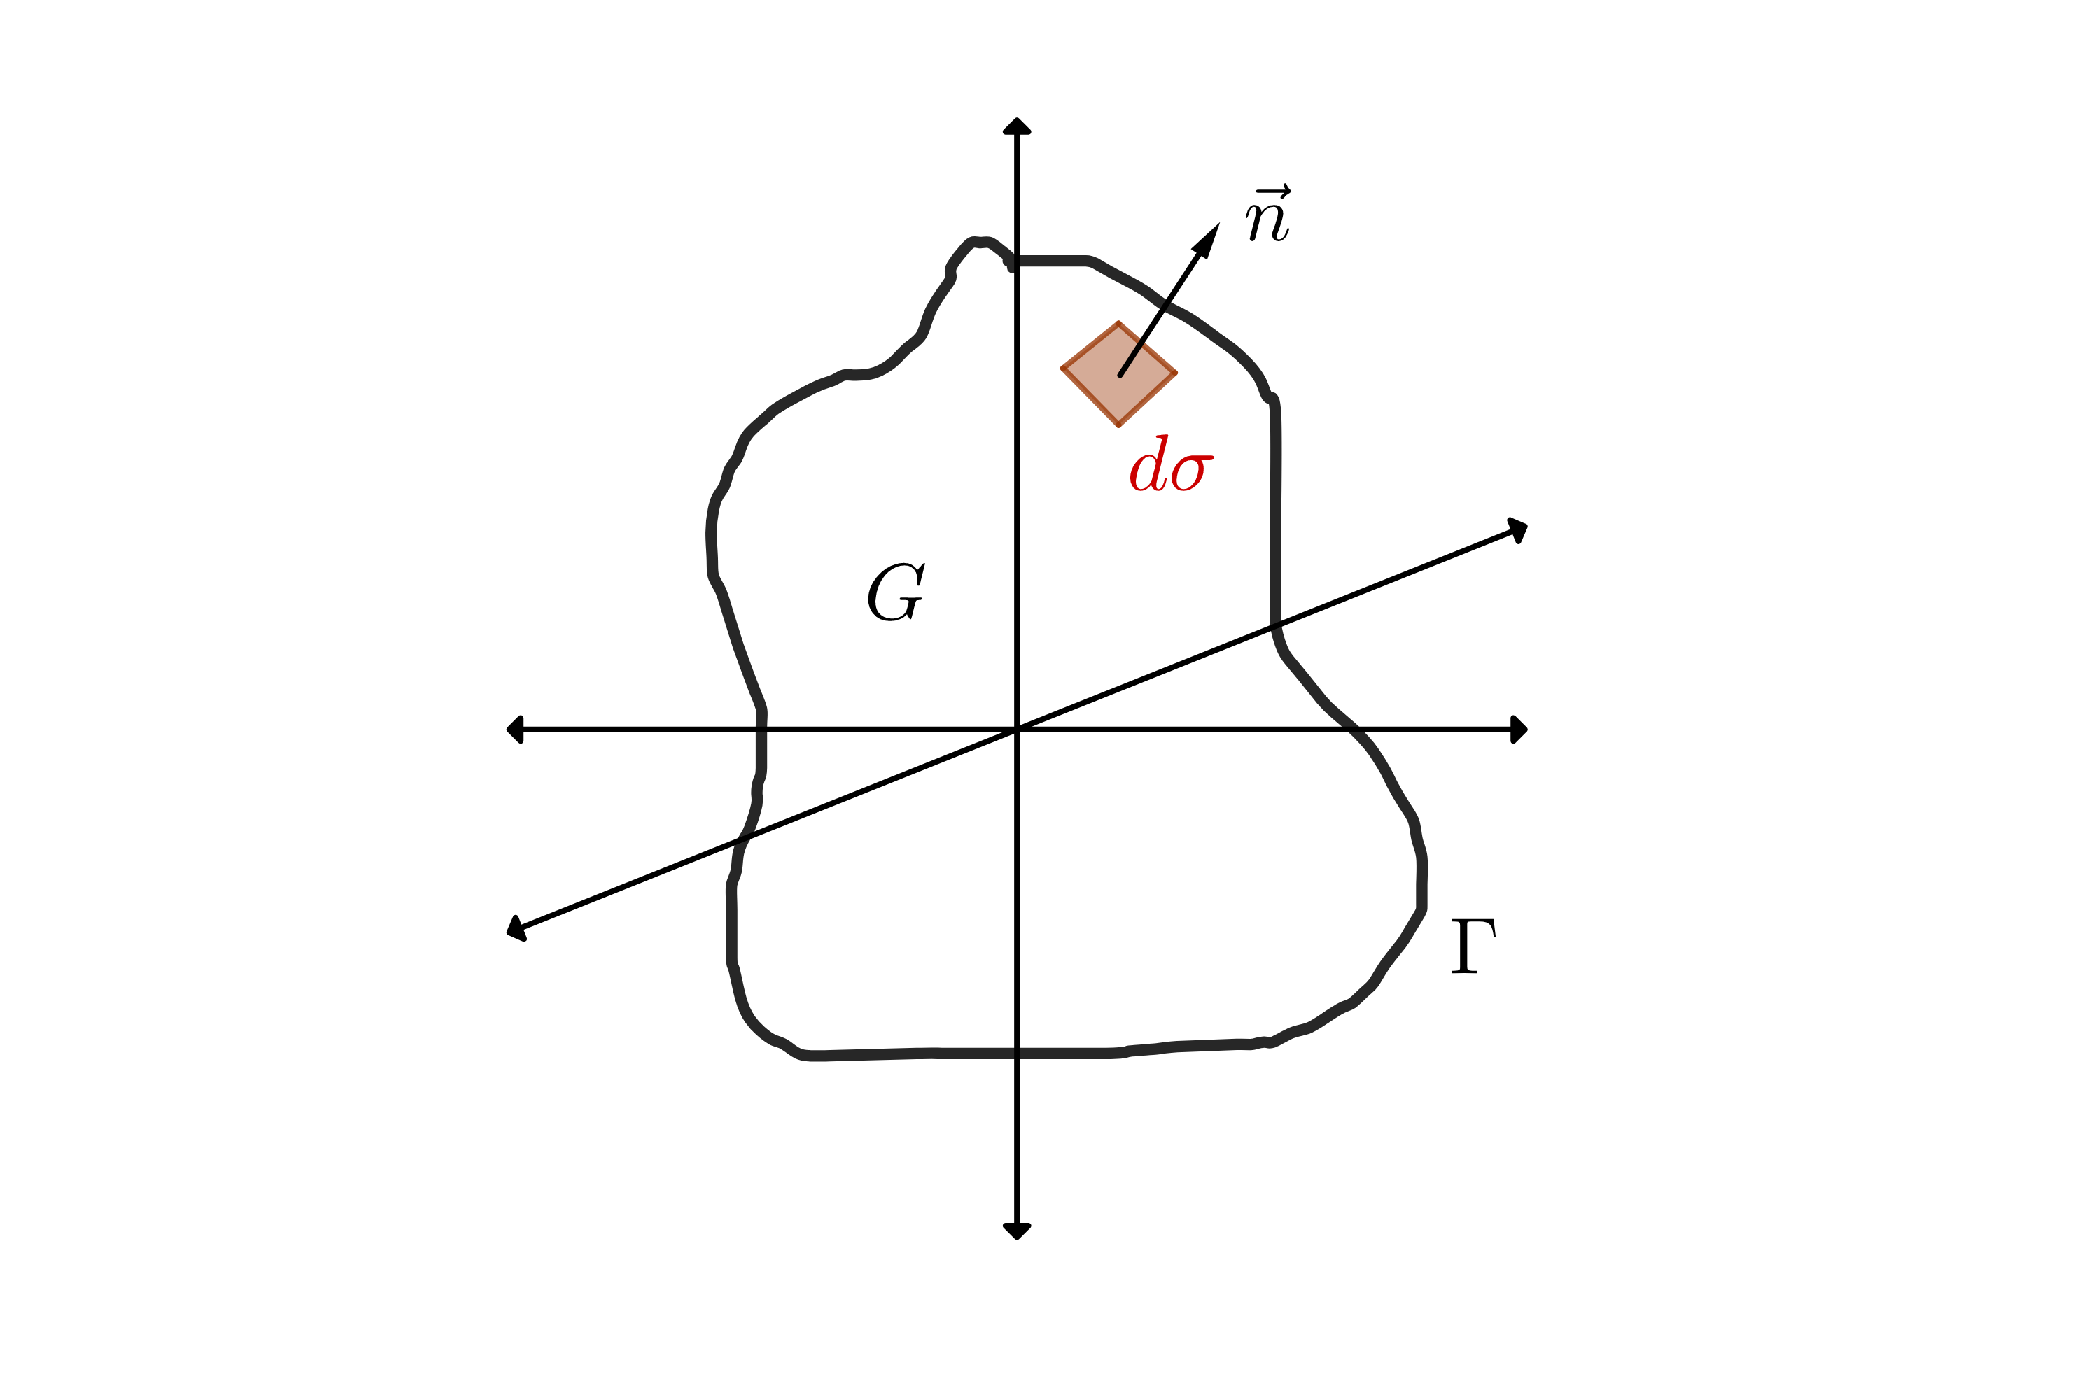
\includegraphics[scale=0.2]{green.png}
\end{center}
for any domain $G$ in three dimensions with boundry $\Gamma$, where the volume element is $dx = dx_1 dx_2 dx_3$, the surface element is $d\sigma$, and $\vec{n}$ is the normal to the surface, let $v(x_1,x_2,x_3)$, $u(x_1,x_2,x_3)$ be functions such that $v,u\in C^3(G)$ and $v,u\in C^2(G\cup \Gamma)$.
\par
now we start our treatment by studying the following diffrentitation. 
\begin{align*}
\frac{\partial }{\partial x_i}\left(v\frac{\partial u}{\partial x_i}\right) &= v\frac{\partial^2 u}{\partial x_{i}^{2}} + \frac{\partial v}{\partial x_i}\frac{\partial u}{\partial x_i}
\\
v\frac{\partial^2 u}{\partial x_{i}^{2}} &= \frac{\partial }{\partial x_i}\left(v\frac{\partial u}{\partial x_i}\right) - \frac{\partial v}{\partial x_i}\frac{\partial u}{\partial x_i}
\end{align*}
intgrating over volume.
\[
    \int_G v\frac{\partial^2 u}{\partial x_{i}^{2}} dx = \int_G \frac{\partial }{\partial x_i}\left(v\frac{\partial u}{\partial x_i}\right) dx - \int_G \frac{\partial v}{\partial x_i}\frac{\partial u}{\partial x_i} dx    
\]
from the divergance theorem we can transform the first integral on the right hand side to a surface integral.
\[
    \int_G v\frac{\partial^2 u}{\partial x_{i}^{2}} dx = \int_\Gamma v\frac{\partial u}{\partial x_i}cos(\vec{n},x_i) d\sigma - \int_G \frac{\partial v}{\partial x_i}\frac{\partial u}{\partial x_i} dx    
\]
summing over i.
\begin{align}
\int_G v\sum_{i=1}^{3}\frac{\partial^2 u}{\partial x_{i}^{2}} dx &= \int_\Gamma v\sum_{i=1}^{3}\frac{\partial u}{\partial x_i}cos(\vec{n},x_i) d\sigma - \sum_{i=1}^{3}\int_G \frac{\partial v}{\partial x_i}\frac{\partial u}{\partial x_i} dx 
\nonumber
\\ 
\int_G v\nabla^2 u dx &= \int_\Gamma v\frac{\partial u}{\partial \vec{n}} d\sigma - \sum_{i=1}^{3}\int_G \frac{\partial v}{\partial x_i}\frac{\partial u}{\partial x_i} dx
\end{align}
in the same manner we can find.
\begin{equation}
\int_G u\nabla^2 v dx = \int_\Gamma u\frac{\partial v}{\partial \vec{n}} d\sigma - \sum_{i=1}^{3}\int_G \frac{\partial u}{\partial x_i}\frac{\partial v}{\partial x_i} dx
\end{equation}
substracting (2) from (1) results in.
\[
    \int_G \left[v\nabla^2 u - u\nabla^2 v\right]dx = \int_\Gamma \left[v\frac{\partial u}{\partial \vec{n}}-u\frac{\partial v}{\partial \vec{n}}\right] d\sigma    
\]
this equation is Green's Identity.

\begin{theorem}[Oleinik's Theorem (maximum principle)]
    if $u(x,y)$ is a harmonic function on G and $u(x,y)$ is continuous on $G \cup \gamma$, then $u(x,y)$ attains its maximum or minimum value on $\gamma$    
\end{theorem}
\begin{proof}
    suppose that the maximum value of u on $G \cup \gamma$ is M, and the minimum value of u on $G \cup \gamma$ is m, then it is clear that $M \geq m$.
    \par
    we want t proof that $M = m$ 
    \par
    suppose that $M > m$ 
    \par
    we first define
    \[
        v(x,y) = u(x,y) + \frac{M-m}{2d^2}\left[(x-x_{1})^2+(y-y_{1})^2\right]    
    \]
    \begin{center}
        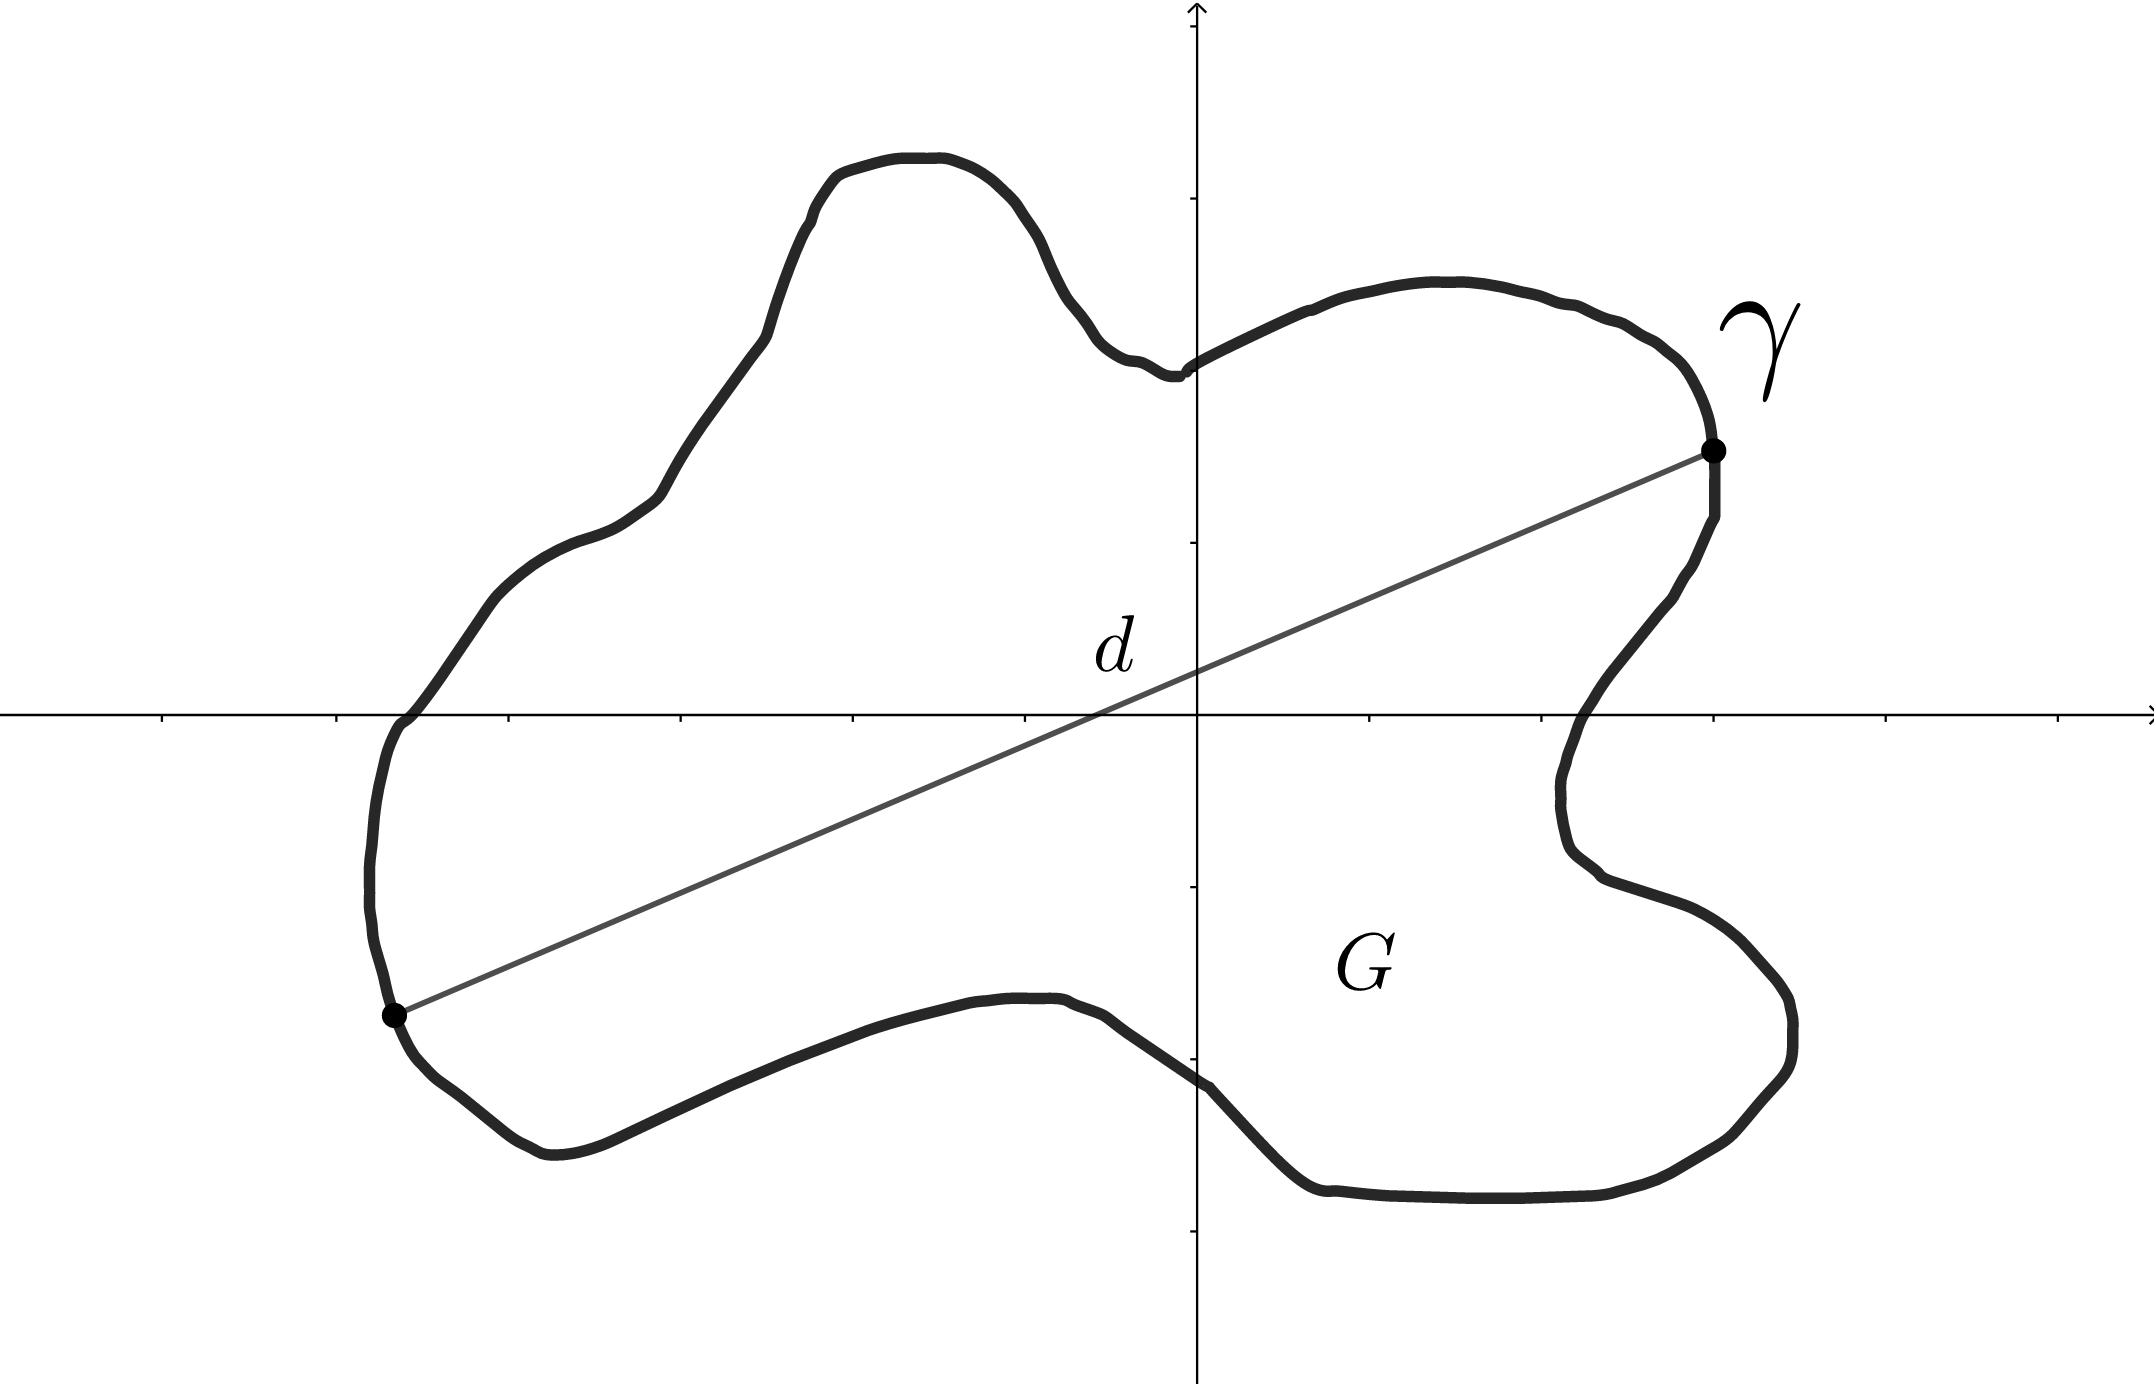
\includegraphics[scale=0.1]{diameter.png}
    \end{center}
    where d is the diameter of the domain G or the longest distance between two point, 
    and $(x_1,y_1)$ is a point inside G such that, $u(x_1,y_1) = M$, thus we have.
    \[
        v(x_1,y_1) = u(x_1,y_1) = M    
    \]
    and on $\gamma$ we find
    \begin{align*}
        v(x,y) &\leq m+\frac{M-m}{2}
        \\
        &\leq \frac{M+m}{2} < \frac{M+M}{2}
        \\
        &< M
    \end{align*}
    this means that v attains a maximum value at a point call it $(x_2,y_2)$ inside G thus we have.
    \[
        \frac{\partial^2 v(x_2,y_2)}{\partial x^2} \leq 0 \;\;\;\;\; \text{and} \;\;\;\;\; \frac{\partial^2 v(x_2,y_2)}{\partial y^2} \leq 0    
    \]
    \[
        \therefore  \nabla^2 v(x_2,y_2) =  \frac{\partial^2 v(x_2,y_2)}{\partial x^2}+\frac{\partial^2 v(x_2,y_2)}{\partial y^2} \leq 0 \dquad \Longrightarrow \circled{1}
    \]
    from the definition of v we obtain
    \begin{align*}
        \frac{\partial^2 v}{\partial x^2} &= \frac{\partial^2 u}{\partial x^2} + \frac{M-m}{d^2}
        \\
        \frac{\partial^2 v}{\partial y^2} &= \frac{\partial^2 u}{\partial y^2} + \frac{M-m}{d^2}
        \\
        \nabla^2 v = \frac{\partial^2 v}{\partial x^2} + \frac{\partial^2 v}{\partial x^2} &= \nabla^2 u + \frac{2(M-m)}{d^2}
        \\
        \because u(x,y) &\text{ is harmonic}\dquad \Longrightarrow \therefore \nabla^2 u = 0
        \\
        \nabla^2 v &= \frac{2(M-m)}{d^2} > 0 \dquad \Longrightarrow \circled{2}
    \end{align*}
    which is a contradiction from \circled{1} and \circled{2} 
    \\
    therefore M $\ngtr$ m therefore M must equal m 
\end{proof}
\begin{theorem}[Uniqueness of Drichlet Problem]
    if there exist a solution of Laplace's equation 
    with a boundary condition (Drichlet problem)
    \[
    \exists u \in C^2(G), u \in C(G \cup \gamma),\;\; \text{such that} \;\;\; \nabla^2 u =0 \;\;\; \text{and} \;\;\; u|_\gamma = f
    \]
    then the solution is unique.
\end{theorem}
\begin{proof}
assuming the two function $u_1$ and $u_2$ are harmonic functions on G with boundary $\gamma$, i.e. 
\[
    u_1 ,u_2 \in C^2(G), u_1 , u_2 \in C(G \cup \gamma), \nabla^2 u_1 =0, \nabla^2 u_2 =0, u_1|_\gamma = f, u_2|_\gamma = f    
\]
we define the function $w$ as follow
\[
    w = u_1-u_2 \Rightarrow w\in C^2(G), w \in C(G \cup \gamma), \nabla^2 w =0, w|_\gamma = f-f = 0    
\]
the value of the function attains its maximum or minimum value on its boundary according to the maximum principle thus we have
\[
    \min(w) = 0 \leq w(x) \leq 0= \max(w) \forall x \in G \;\;\;\; thus \;\;\;\; w = 0 \Rightarrow u_1 = u_2     
\]
\end{proof}

\begin{theorem}[Stability Theorem]
    supposing the two functions $u_1$, $u_2$, are harmonic on domain G with boundary $\gamma$, and have the boundary conditions, 
    \\
    $u_1|_\gamma = f_1$ and $u_2|_\gamma = f_2$, if $|f_1 - f_2| \leq \epsilon  \;\;\; \forall \epsilon > 0$ then $|u_1(x) - u_2(x)| \leq \epsilon \;\;\; \forall x \in G \cup \gamma $
\end{theorem}
\begin{proof}
    according to he maximum principle $-\epsilon \leq u_1 - u_2 \leq \epsilon \;\;\; \Rightarrow \;\;\; |u_1 - u_2| \leq \epsilon$
\end{proof}

\begin{enrichment*}{Potential Function}
    The inverse square law's occurrence is frequent in physics, most notably in the classical theory of gravitation where the gravitational force is inversly proportional to the square of the sepration between two masses.
\[
    F_g = G\frac{m_1 m_2}{r^2}    
\]
and in classical electrostatics where cloumb's law for the electrical force between stationary charges is.
\[
    F_e = K\frac{q_1 q_2}{r^2}    
\]
in general we find that $F \propto \frac{1}{r^2}$ is frequently occuring in physics and since the potential energy is the intgration of force
= $\displaystyle -\int F dr$ we find that potential energy is porportioanl to the inverse of or sepration distance $PE \propto \frac{1}{r}$, thus the need for studying such functions is as important as potential energy which showed to be very important.
\par
now we define a general function called E which is porportioanl to the inverse of or sepration, the most general will be.
\[
    E(x,y) = \frac{1}{r}\;\;,\;\;\;\;\;\;\; where\;\;\;\;\; r = \sqrt{(y_1-x_1)^2 + (y_2-x_2)^2 + (y_2-x_2)^2}    
\]
It is easy to show that E is harmonic on $\mathbb{R}^3$.
\[
    \nabla_{x}^{2} E(x,y) = 0 \tquad \text{and} \tquad \nabla_{y}^{2} E(x,y) = 0    
\]
where $\nabla_{x}^{2}$ and $\nabla_{y}^{2}$ is the laplacean with resprect to x and y respectivly
\end{enrichment*}

\setcounter{equation}{0}
\subsection{Representation formula}
We will utilize Green's identity and the potential function for solving Laplace's equation Drichlet problem. Due to the singularity of the potential function an issue arises, thus we will apply the identity to the pair of functions u and E on the region G with a sphere of radius $\epsilon$ cutout with the singularity being the center of the sphere, then take the limit of $\epsilon$ to zero to find our final answer.
\begin{figure}[h]
\begin{center}
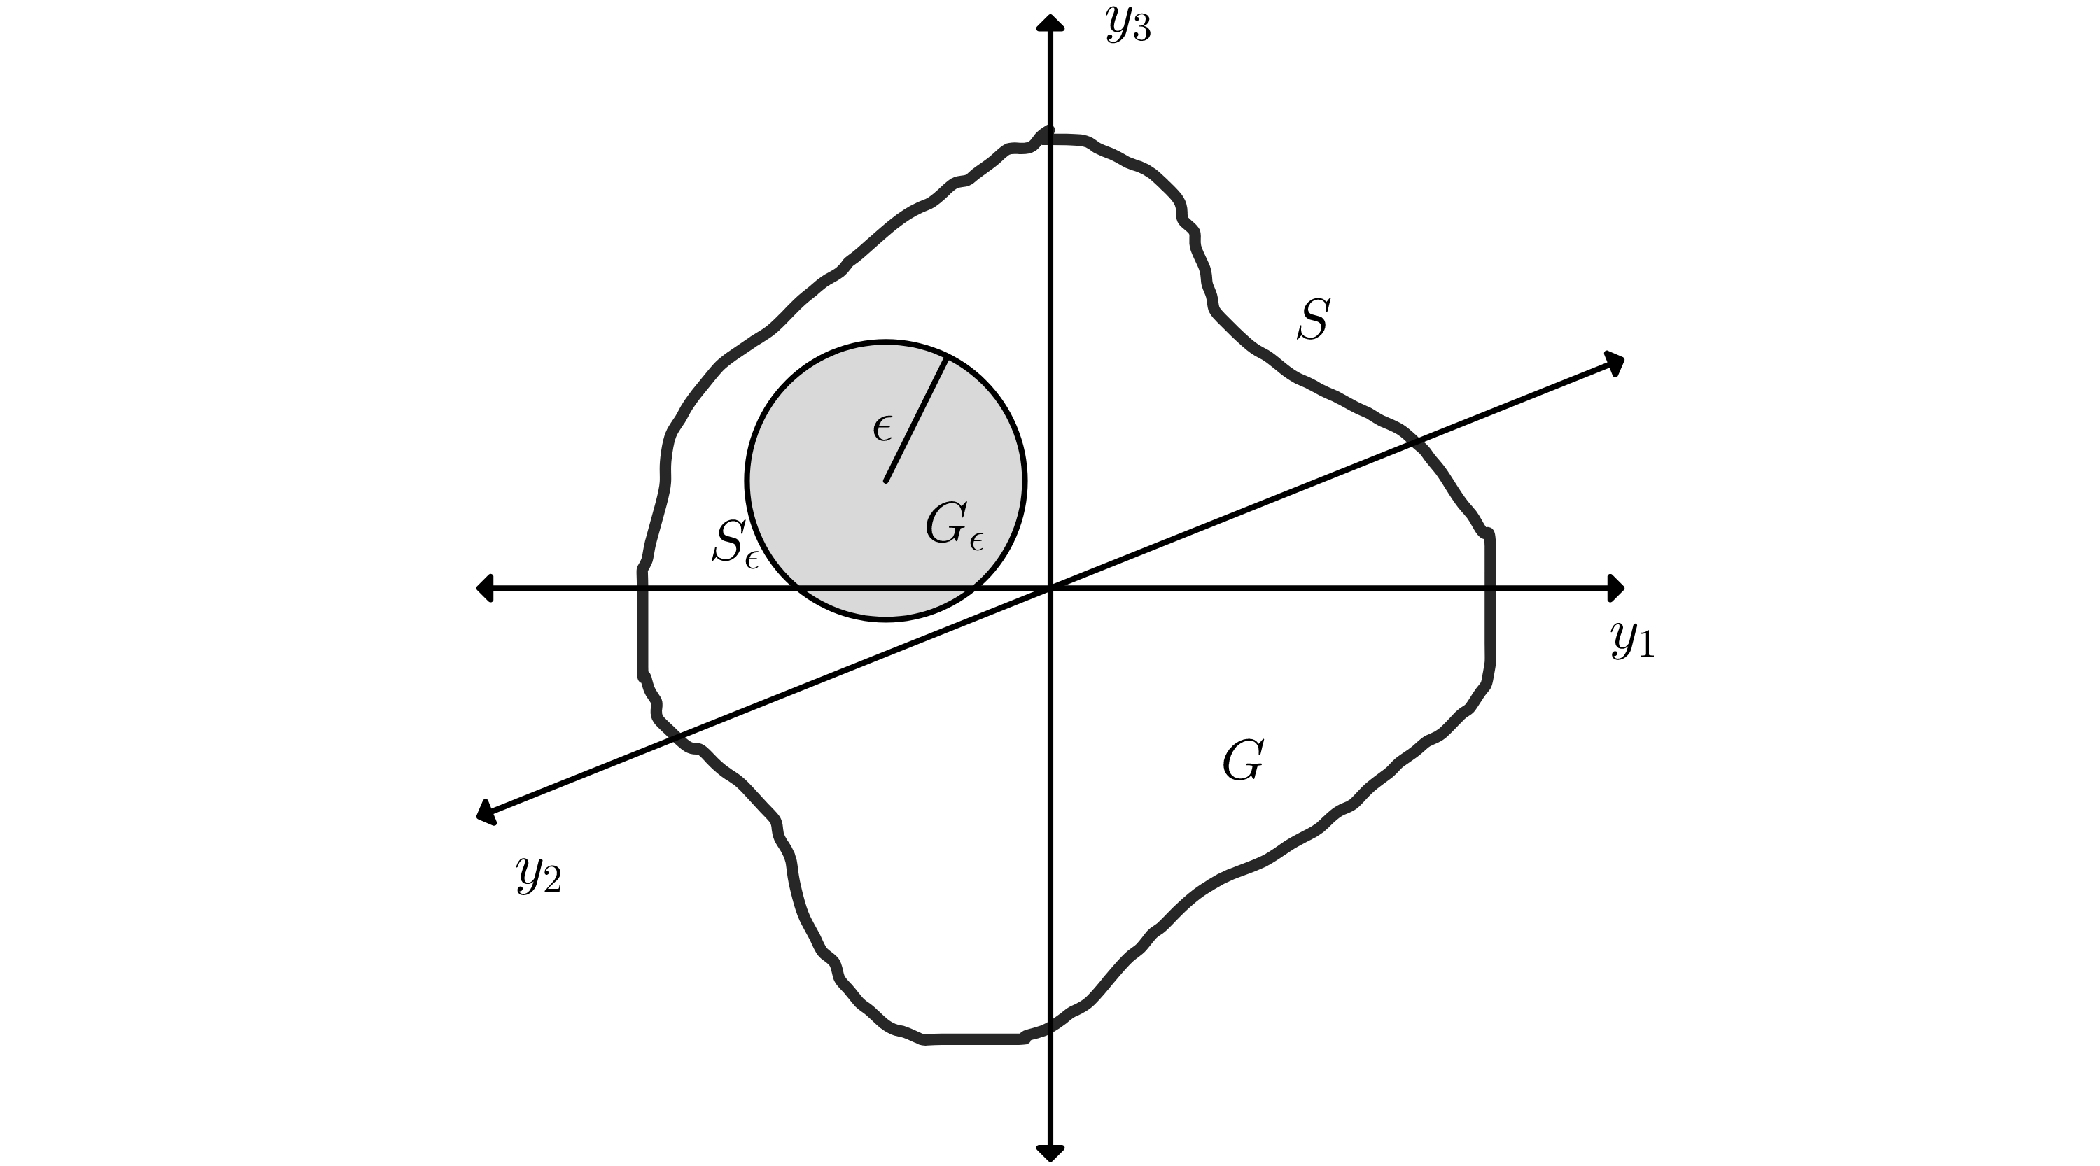
\includegraphics[scale=0.15]{rep.png}
\captionlabelfalse
\caption{the domian}
\end{center}
\end{figure}
the domain $G$ is any contineous closed volume, with surface $S$, the domain $G_\epsilon$ is a sphere inside our volume, i.e. $G_\epsilon \in G$, with its center $x = (x_1,x_2,x_3)$, radius $\epsilon$, and surface $S_\epsilon$. 
\begin{align}
\nabla_{y}^{2} u(y) =0
\end{align}
where
\begin{align}
u(y) \in C^3(G)\;,\;\;\; u(y) \in C^2(G\cup S)
\end{align}
from (2) the condition for using Green's identity between the pair of function u and the potential function E is satisfyed since they are both contineous on our domain. Thus using the identity yeilds.
\[
    \int_G \left[E(x,y)\nabla_{y}^{2} u(y) - u(y)\nabla_{y}^{2} E(x,y)\right]dx = \int_\Gamma \left[E(x,y)\frac{\partial u(y)}{\partial \vec{n}}-u(y)\frac{\partial E(x,y)}{\partial \vec{n}}\right] d\sigma    
\]
\[
  \because \nabla_{y}^{2} E(x,y) = 0    
\]
and from (1) we get that the left hand side is zero then we get.
\[
    \int_\Gamma \left[E(x,y)\frac{\partial u(y)}{\partial \vec{n}}-u(y)\frac{\partial E(x,y)}{\partial \vec{n}}\right] d\sigma = 0    
\]
since a sphere cutout was proposed then our region of study has two surfaces with the normal being opposite in direction thus the surface integral at hand can be split in two and we get.
\[
    \int_S \left[E(x,y)\frac{\partial u(y)}{\partial \vec{n}}-u(y)\frac{\partial E(x,y)}{\partial \vec{n}}\right] d\sigma - \int_{S_\epsilon} \left[E(x,y)\frac{\partial u(y)}{\partial \vec{n_\epsilon}}-u(y)\frac{\partial E(x,y)}{\partial \vec{n_\epsilon}}\right] d\sigma_\epsilon  = 0    
\]
the first term in the second intgral vanishes due to spherical symmetry, 
\\and on $S_\epsilon$ we have $r=\epsilon$ then $E = \frac{1}{\epsilon}$ therefore $\displaystyle \frac{\partial E(x,y)}{\partial \vec{n_\epsilon}} = \frac{\partial}{\partial \epsilon}\frac{1}{\epsilon} = -\frac{1}{\epsilon^2}$
thus we are left with.
\[
    \int_S \left[E(x,y)\frac{\partial u(y)}{\partial \vec{n}}-u(y)\frac{\partial E(x,y)}{\partial \vec{n}}\right] d\sigma  = \frac{1}{\epsilon^2} \int_{S_\epsilon} u(y) d\sigma_\epsilon    
\]
by adding and subtracting $\displaystyle \frac{1}{\epsilon^2} \int_{S_\epsilon} u(x) d\sigma_\epsilon$ the following term from the right hand side.
\begin{align}
\int_S \left[E(x,y)\frac{\partial u(y)}{\partial \vec{n}}-u(y)\frac{\partial E(x,y)}{\partial \vec{n}}\right] d\sigma  &= \frac{1}{\epsilon^2} \left[\int_{S_\epsilon} (u(y) - u(x)) d\sigma_\epsilon + \int_{S_\epsilon} u(x) d\sigma_\epsilon\right]
\end{align}
we now show that the first integral on the right hand side vanishes as $\epsilon \to 0$.
\[
    \left|\int_{S_\epsilon} u(y)-u(x) d\sigma_\epsilon \right| \leq \int_{S_\epsilon} |u(y)-u(x)| d\sigma_\epsilon \leq \delta(\epsilon)\int_{S_\epsilon} d\sigma_\epsilon \leq 4\pi \delta(\epsilon)    
\]
as $\epsilon \to 0$ , $\delta(\epsilon) \to 0$
\\because the absolute value of the integral is $\leq$ 0 then it's equal 0. Now we evalute the second integral.
\[
    \int_{S_\epsilon} u(x)d\sigma_\epsilon = u(x)\int_{S_\epsilon}d\sigma_\epsilon = u(x) 4\pi\epsilon^2
\]
substituting in (3) we finally get the representation formula
\[
    u(x) = \frac{1}{4\pi} \int_S \left[E(x,y)\frac{\partial u(y)}{\partial \vec{n}}-u(y)\frac{\partial E(x,y)}{\partial \vec{n}}\right] d\sigma    
\]

\begin{enrichment*}{Hanckel Transform}
    let $f$ be a function in $r$ on the interval $[0,\infty]$, then the Hanckel transform is defined as.
    \[
        \hat{f}(\rho) = \int_{0}^{\infty} r J_o(r\rho) f(r) dr    
    \]
    where $J_o$ is the Bessel function 
    \[
        J_o(z) = \frac{1}{2\pi}\int_{0}^{\infty} \cos(zcos\theta)d\theta     
    \]
    which has the property 
    \[
        z J_o''(z) + J_o'(z)+ zJ_o(z) = 0     
    \]
    and the inverse Hanckel Transform is 
    \[
        f(r) = \int_{0}^{\infty} \rho J_o(r\rho) \hat{f}(\rho) d\rho    
    \]
\end{enrichment*}
\setcounter{equation}{0}
\subsection{Laplace's Equation in Cylinderical Coordinates}
considering the Drichlet problem.
\begin{equation}
\nabla^2 u(r,z) = \frac{\partial^2 u(r,z)}{\partial z^2} + \frac{1}{r}\frac{\partial}{\partial r}\left[r\frac{\partial u(r,z)}{\partial r}\right] = 0 \;\; , \;\;\; r >0
\end{equation}
\begin{equation}
\text{I.C} \quad \Longrightarrow \quad u(r,0) = f(r)
\end{equation}
\begin{equation}
\text{B.C} \quad \Longrightarrow \quad \lim_{r\rightarrow\infty} u(r,z) =0
\end{equation}
by taking Hankel transformation for equation (1) 
\begin{align*}
\frac{\partial^2 }{\partial z^2}\int_{0}^{\infty} rJ_o(r\rho)u(r,z) dr &+ \int_{0}^{\infty}rJ_o(r\rho)\frac{1}{r}\frac{\partial}{\partial r}\left[r\frac{\partial u(r,z)}{\partial r}\right]dr = 0
\\
\frac{\partial^2 \hat{u}(\rho,z)}{\partial z^2} &+ \int_{0}^{\infty}J_o(r\rho)\frac{\partial}{\partial r}\left[r\frac{\partial u(r,z)}{\partial r}\right]dr = 0
\end{align*}
\begin{equation}
\frac{\partial^2 \hat{u}(\rho,z)}{\partial z^2}  = -\int_{0}^{\infty}J_o(r\rho)\frac{\partial}{\partial r}\left[r\frac{\partial u(r,z)}{\partial r}\right]dr
\end{equation}

\newpage 

now we write the right hand side as.
\begin{align*}
-\int_{0}^{\infty}J_o(r\rho)\frac{\partial}{\partial r}\left[r\frac{\partial u(r,z)}{\partial r}\right]dr &= -\int_{0}^{\infty}\frac{\partial}{\partial r}\left[J_o(r\rho)r\frac{\partial u(r,z)}{\partial r}\right]dr + \int_{0}^{\infty} r\frac{\partial u(r,z)}{\partial r} \rho J_o'(r\rho)dr
\\
&= -\left[rJ_o(r\rho)\frac{u(r,z)}{\partial r}\right]_{0}^{\infty} + \int_{0}^{\infty} r\rho\frac{\partial u(r,z)}{\partial r} J_o'(r\rho)dr
\\
&= \int_{0}^{\infty} r\rho\frac{\partial u(r,z)}{\partial r} J_o'(r\rho)dr
\end{align*}
the first term vanishes since Bessel functions tend to zero when r approaches infinity
\begin{align*}
\int_{0}^{\infty} r\rho\frac{\partial u(r,z)}{\partial r} J_o'(r\rho)dr
&= \int_{0}^{\infty} \frac{\partial}{\partial r}\left[ r\rho\frac{\partial u(r,z)}{\partial r} J_o'(r\rho)\right]dr 
- \int_{0}^{\infty} \left[\rho J_o'(r\rho)+ r\rho^2 J_o''(r\rho)\right] u(r,z)dr
\\
&= \left[ r\rho\frac{\partial u(r,z)}{\partial r} J_o'(r\rho)\right]_{0}^{\infty} - \int_{0}^{\infty} \frac{1}{r}\left[r\rho J_o'(r\rho)+ r^2\rho^2 J_o''(r\rho)\right] u(r,z)dr
\\
&= - \int_{0}^{\infty} \frac{1}{r}\left[r\rho J_o'(r\rho)+ r^2\rho^2 J_o''(r\rho)\right] u(r,z)dr
\end{align*}
from the bassel function property we get.
\begin{align*}
- \int_{0}^{\infty} \frac{1}{r}\left[r\rho J_o'(r\rho)+ r^2\rho^2 J_o''(r\rho)\right] u(r,z)dr &= \int_{0}^{\infty} \frac{1}{r}\left[r^2\rho^2 J_o(r\rho)\right] u(r,z)dr
\\
&= \rho^2 \int_{0}^{\infty} r J_o(r\rho) u(r,z)dr
\\
&= \rho^2 \hat{u}(\rho,z)
\end{align*}
therefore we can get.
\[
    \frac{\partial^2 \hat{u}(\rho,z)}{\partial z^2} = \rho^2 \hat{u}(\rho,z)    
\]
which have the solution. 
\[
\hat{u}(\rho,z) = A e^{\rho z} + Be^{-\rho z}    
\]
and from the boundary condition after taking the Hankel transformation for it $\hat{u}(\rho,z)$ is convergent at $\rho \to \infty$
\[
\therefore A = 0    
\]
and preforming the Hankel transorm on the initial condition.
\[
\hat{u}(\rho,0) = B = \hat{f}(\rho)    
\]
\[
\hat{u}(\rho,z) = \hat{f}(\rho)e^{-\rho z}    
\]
now to find u we preform the inverse Hankel Transform.
\[
u(r,z) = \int_{0}^{\infty} \rho J_o(r\rho)\hat{f}(\rho)e^{-\rho z} d\rho    
\]

\newpage
\setcounter{equation}{0}
\section{Burger's Equation}

Burger's equation  is a fundamental partial differential equation occurring in various areas of applied mathematics. It has many forms, we will be studying the solution of one of its forms; the viscous Burger's equation Cauchy problem, occurying in fluid dynamics, , the viscous equation is non linear thus needs a different approuch than those used earlier. We will be using the method of Hopf-Cole.

\begin{equation}
\frac{\partial u(x,t)}{\partial t} + u(x,t)\frac{\partial u(x,t)}{\partial x} = \gamma \frac{\partial^2 u(x,t)}{\partial x^2} \tquad \gamma > 0 , x \in \mathbb{R}
\end{equation}
\begin{equation}
\text{I.C} \quad \Longrightarrow \quad u(x,0) = f(x)
\end{equation}
\begin{enrichment*}{}
    if $\gamma = 0$ the equation is called the inviscous Burger's equation
\end{enrichment*}
we start our treatment by defining a new function
\[
v(x,t) = e^{\alpha\phi(x,t)}    
\]
\[
\phi(x,t) = \frac{1}{\alpha}\ln(v(x,t))    
\]
we try to find the function $\phi$ such that $v$ satisfy
\begin{equation}
\frac{\partial v}{\partial t} = \gamma \frac{\partial^2 v}{\partial x^2}
\end{equation}
\begin{equation*}
\text{I.C} \quad \Longrightarrow \quad v(x,0) = g(x)
\end{equation*}
we start finding the terms of the equation (3) in terms of $\phi$
\begin{align*}
\hspace{2cm}
\frac{\partial v}{\partial t} &= \alpha e^{\alpha\phi} \frac{\partial \phi}{\partial t}
\\
\frac{\partial v}{\partial x} &= \alpha e^{\alpha\phi} \frac{\partial \phi}{\partial x} 
\\
\frac{\partial^2 v}{\partial x^2} &= \alpha^2 e^{\alpha \phi} {\left(\frac{\partial \phi}{\partial x}\right)}^2 + \alpha e^{\alpha\phi} \frac{\partial^2 \phi}{\partial x^2}
\end{align*}
substitute in (3)
\begin{align}
\alpha e^{\alpha\phi} \frac{\partial \phi}{\partial t} &= \gamma\left(\alpha^2 e^{\alpha \phi} {\left(\frac{\partial \phi}{\partial x}\right)}^2 + \alpha e^{\alpha\phi} \frac{\partial^2 \phi}{\partial x^2}\right)\nonumber
\\
\frac{\partial \phi}{\partial t} &= \gamma\alpha {\left(\frac{\partial \phi}{\partial x}\right)}^2 + \gamma \frac{\partial^2 \phi}{\partial x^2}
\end{align}
diffrentiating the equation (4) with respect to x and changing the order of diffrentiation on the left hand side
\[
    \frac{\partial }{\partial t}\left[ \frac{\partial \phi}{\partial x}\right] = 2\gamma\alpha \frac{\partial\phi}{\partial x}\frac{\partial^2 \phi }{\partial x^2} + \gamma\frac{\partial^3 \phi}{\partial x^3}    
\]
now put $\displaystyle u(x,t) = \frac{\partial \phi(x,t)}{\partial x}$
\[
    \frac{\partial u }{\partial t} = 2\gamma\alpha u\frac{\partial u}{\partial x} + \gamma\frac{\partial^2 u}{\partial x^2}    
\]
set $2\gamma\alpha = -1$ we get
\[
    \frac{\partial u }{\partial t} + u\frac{\partial u}{\partial x} = \gamma\frac{\partial^2 u}{\partial x^2}    
\]
means that $\displaystyle \frac{\partial \phi(x,t)}{\partial x}$ is a solution for the burger equation 

we know that problem (3) is the heat equation cauchy problem that we solved before using Poisson's formula and we know that the solution is 
\[
v(x,t) = \frac{1}{\sqrt{4\pi \gamma t}} \int_{-\infty}^{\infty} e^{-\frac{(x-y)^2}{4\gamma t}} g(y)dy    
\]
finding v we can now find $\phi$ from the relation $\displaystyle \phi(x,t) = \frac{1}{\alpha}\ln(v(x,t))$ then diffrentiating it with respect to x to finally find u.

\section{Integral Equations}
\
\begin{definition}[Integral equations]
    are equations in which an unknown function appears under an integral sign.
\end{definition}
There is a close connection between differential and integral equations, and some problems may be formulated either way.

\subsection{Successive Approximation}
\
\begin{definition}[Successive Approximation Method]
    is a numerical technique used to solve equations or find the roots of functions that cannot be solved analytically. It is an iterative process in which you start with an initial guess for the solution and then repeatedly refine that guess to get closer and closer to the actual solution.
\end{definition}

Here's a step-by-step explanation of the successive approximation method:

\begin{enumerate}[itemsep=10pt]
    \item \textbf{Formulate the Equation}: Start with the equation you want to solve or the function for which you want to find the root. For example, let's say you want to find the root of the equation $f(x)=0$.
    \item \textbf{Choose an Initial Guess}: Pick an initial guess for the root. This can be any value that you think is close to the actual root. The quality of your initial guess can affect the convergence speed of the method.
    \item \textbf{Update the Guess}: Use the chosen initial guess and the equation (or function) to calculate an updated value, which will be a new approximation for the root. Let's call this updated value $x_1$.
    \item \textbf{Check for Convergence}:Determine if the updated value $x_1$ is close enough to the actual root. If it's not, go back to step 3 and repeat the process using $x_1$ as the new guess. Keep iterating until the solution converges to the desired accuracy.
    \item \textbf{Termination Criteria}:Decide on a termination condition to stop the iterations. This condition could be a maximum number of iterations or reaching a desired level of accuracy (e.g.,$|x_1-x_0|<\epsilon$ , where $\epsilon$ is a small tolerance value).
    \item \textbf{Final Result}: Once the termination condition is met, the value obtained in the last iteration is considered the approximation of the root.
\end{enumerate}
The successive approximation method is straightforward to implement and can be used for a wide range of equations and functions. However, its convergence may not always be guaranteed, especially if the function has complex behavior or multiple roots. In such cases, other numerical methods like the Newton-Raphson method or the bisection method may be more appropriate.

It's also essential to be cautious with the choice of the initial guess, as an inappropriate initial value might lead to divergence or convergence to a different root. Experimenting with different initial guesses can help you achieve better results.

In the context of integral equations, the successive approximation method is a powerful technique for solving integral equations of the form:
\[
\phi(x) = f(x) + \lambda\int_{a}^{b} K(x,t) \phi(t)dt    
\]
where $\phi(x)$ is the unknown function to be determined,
$f(x)$  is a given function, $K(x,y)$ is the kernel of the integral equation,
and $\lambda$ is a constant parameter.

The successive approximation method is an iterative approach that allows us to find an approximate solution to this integral equation by breaking it down into simpler steps. Here's how it works:

\begin{enumerate}[itemsep=10pt]
    \item \textbf{Formulate the Integral Equation}: Write down the integral equation in the form mentioned above, making sure you have a well-defined kernel $K(x,y)$ and a given function $f(x)$ 
    \item \textbf{Choose an Initial Guess}: Start with an initial guess for the unknown function $\phi(x)$. This guess can be any reasonable function that satisfies any known boundary or initial conditions.
    \item \textbf{Update the Guess}: Substitute the initial guess for $\phi(x)$ into the integral equation and calculate an updated function $\phi_1(x)$ :
    \[
       \phi_1(x) = f(x) + \lambda\int_{a}^{b} K(x,t) \phi(t)dt     
    \]
    \item \textbf{Check for Convergence}:Check the difference between the updated function $\phi_1(x)$ and the previous approximation. If the difference is below a certain tolerance level or satisfies a convergence criterion, stop the iterations and consider $\phi_1(x)$ as the final approximation. Otherwise, continue to the next step.
    \item \textbf{Repeat the Process}: Use $\phi_1(x)$ as the new approximation and repeat the process. Substitute $\phi_1(x)$ into the integral equation to find a new approximation $\phi_2(x)$ , and so on. Continue iterating until the solution converges to the desired accuracy.
    \item \textbf{Termination Criteria}:Decide on a termination condition to stop the iterations, similar to the termination criteria in the general successive approximation method. This could be based on a maximum number of iterations or reaching a desired level of accuracy.    
    \item \textbf{Final Result}: Once the termination condition is met, the last obtained approximation $\phi_n(x)$ is considered the solution to the integral equation.
\end{enumerate}
It's important to note that the convergence of the successive approximation method for integral equations depends on various factors, including the nature of the kernel $K(x,y)$, the choice of the initial guess, and the value of the parameter 
$\lambda$. In some cases, convergence may be slow or may not occur at all. In such situations, other numerical methods tailored for specific types of integral equations may be more appropriate.

\newpage 




\subsection{Fredholm's Integral Equation}
consider the following intgral equation.
\[
u(x) = f(x) + \lambda\int_{a}^{b} k(x,y) u(y)dy    
\]
where $f(x)$ and $k(x,y)$ are given contineous function on $[a,b]\times[c,d]$ and
\[
    G 
    \begin{cases}
    (x,y) |&     a\leq x\leq b \quad \text{and} \quad c\leq y\leq d
    \end{cases}
\]
we try to determine the function $u(x)$ using the successive approximation method.
\begin{align*}
u_1(x) &= f(x) + \lambda\int_{a}^{b} k(x,y) u_o(y)dy
\\
u_2(x) &= f(x) + \lambda\int_{a}^{b} k(x,y) u_1(y)dy
\\
\vdots
\\
u_{n+1}(x) &= f(x) + \lambda\int_{a}^{b} k(x,y) u_n(y)dy
\end{align*}
let us choose.
\[
u_o(x) = f(x)    
\]
then.
\begin{align*}
u_1(x) &= u_o(x) + \lambda\int_{a}^{b} k(x,y) u_o(y)dy
\\
u_1(x)- u_o(x) &= \lambda\int_{a}^{b} k(x,y) u_o(y)dy
\end{align*}
since the intgral is defenite and the functions are contineous on the limits of intgration 
this can be considerd as the inner product of the two functions 
with will be less than or equal to their magnitudes where $|k(x,y)| = M$ and $|f(x)| = m$.
\begin{enrichment*}{}
    the inner product of two functions on the space of continous functions is defined as 
    \[
        <f,g> = \int f(x)g(x)dx \leq |f(x)||g(x)|
    \]
     remmber the inner product of vectors $\vec{v}\cdot \vec{u} = vu \cos(\theta) \leq vu$
\end{enrichment*}
\begin{align*}
    \left|u_1(x)- u_o(x)\right| &= |\lambda|\left|\int_{a}^{b} k(x,y) u_o(y)dy\right|    
    \\
    & \leq |\lambda|\int_{a}^{b}|k(x,y)||u_o(y)|dy = |\lambda|Mm\int_{a}^{b}dy
    \\
    & \leq |\lambda|Mm(b-a)
\end{align*}
we also have in the same manner. 
\begin{align*}
u_2(x) &= f(x) + \lambda\int_{a}^{b} k(x,y) u_1(y)dy
\\
u_2(x) - u_1(x)&= \lambda\int_{a}^{b} k(x,y) [u_1(y)-u_o(y)]dy
\\
|u_2(x) - u_1(x)| &= |\lambda|\left|\int_{a}^{b} k(x,y) [u_1(y)-u_o(y)]dy\right| 
\\
&\leq |\lambda|Mm(b-a) M \int_{a}^{b}dy = |\lambda|^2M^2{(b-a)}^2 m
\end{align*}
and by induction we can find.
\[
    |u_{k}(x) - u_{k-1}(x)| \leq |\lambda|^kM^k {(b-a)}^k m    
\]
we note that.
\begin{align*}
u_o(x) + \sum_{k=1}^{n} [u_{k}(x) - u_{k-1}(x)] &= u_o + u_1 - u_o + u_2 - u_1 + u_3 - u_2 + ...+u_n - u_{n-1}
\\
&= u_n(x)
\end{align*}
we can find the solution $u(x)$ by taking the limit to $\infty$
\[
    \lim_{n\to\infty} u_n(x) = u(x) = u_o(x) + \sum_{k=1}^{\infty} [u_{k}(x) - u_{k-1}(x)] \leq u_o(x) + m\sum_{k=1}^{\infty} {(|\lambda|M(b-a))}^k    
\]
this is geometric series
if $|\lambda|M(b-a) < 1$ then the series converges absolutly and uniformally
\begin{example}
    Consider the Fredholm integral equation 
    \[
        u(x) = e^x + e^{-1}\int_{0}^{1}u(y)dy    
    \]
    we can select any real value function for the zeroth component then we set 
    \[
    u_0(x) = e^x 
    \]
    now to get $u_1(x)$
    \[
        u_1(x) = e^x + e^{-1}\int_{0}^{1}u_0(y)dy        
    \]
    and that gives us the first approximation of $u(x)$ by
    \[
        u_1(x) = e^x + 1 - e^{-1} 
    \]
    now to get $u_2(x)$
    \[
        u_2(x) = e^x + e^{-1}\int_{0}^{1}e^ydy = e^x + 1 - e^{-2}
    \]
    this gives us the second approximation of $u(x)$
    \\
    continue in the same manner we find the third approximation of $u(x)$
    \[
        u_3(x) = e^x + 1 - e^{-3}
    \]
    proceeding as before we can obtain the n-th component
    \[
        u_n(x) = e^x + 1 - e^{-n} , \quad n \geq 1
    \]
    now to get the solution taking the limit to $\infty$
    \begin{align*}
        u(x) &= \lim_{n\to\infty} u_n(x)
        \\
        &= \lim_{n\to\infty} e^x + 1 - e^{-n}
        \\
        &= e^x + 1
    \end{align*}
\end{example}
\begin{example}
    Consider the Fredholm integral equation 
    \[
        u(x) = x + \lambda\int_{0}^{1} xt u(t)dt
    \]
    for the zeroth component we set 
    \[
    u_0(x) = x
    \]
    then we get get $u_1(x)$
    \[
        u_1(x) = x + \lambda\int_{0}^{1} xt^2dt
    \]
    and that gives us the first approximation of $u(x)$ by
    \[
        u_1(x) = x + \frac{\lambda}{3}x
    \]
    now to get $u_2(x)$
    \[
        u_2(x) = x + \lambda\int_{0}^{1} xt\left(t + \frac{\lambda}{3}t\right)dt = x +\frac{\lambda}{3} x +\frac{\lambda^2}{9} x
    \]
    this gives us the second approximation of $u(x)$
    \\
    proceeding as before we can obtain the n-th component
    \[
        u_n(x) = x +\frac{\lambda}{3} x +\frac{\lambda^2}{9} x + \dots + \frac{\lambda^{n-1}}{3^{n-1}} x , \quad n \geq 1
    \]
    \[
        u_n(x) = x\sum_{k=0}^{n} {\left(\frac{\lambda}{3}\right)}^{k}
    \]
    now to get the solution taking the limit to $\infty$
    \begin{align*}
        u(x) &= \lim_{n\to\infty} u_n(x)
        \\
        &= x\sum_{k=0}^{\infty} {\left(\frac{\lambda}{3}\right)}^{k}
    \end{align*}
    this is geometric series if $|\lambda| < 3$ and $\lambda \neq 0$ it's value will be 
    \[
    u(x) = \frac{3}{3-\lambda}x, \quad  |\lambda| < 3,\lambda \neq 0
    \]
\end{example}
\subsection{Volttera Integral Equation}
Volterra integral equations have wide applications in areas like control theory, population dynamics, signal processing, and modeling dynamic systems. Different forms of the equation, such as Volterra integral equations of the second kind, exist to address specific scenarios and applications.
\par 
consider the following  integral equation.
\[
u(x) = f(x) + \int_{0}^{x} K(x,y) u(y)dy
\]
where the functions $f(x)$ is a given function, often called the "forcing function" or "input function."
and $k(x,y)$ is a given kernel function
\\
To solve this equation we use, as we did with Fredholm's intergral equation, the method f succssive approximation. We first define a sequence.
\[
u_n(x) = f(x) + \int_{0}^{x} K(x,y) u_{n-1}(y)dy    
\]
we can choose our first term arbitrarly but here we choose it to be $u_0(x) = f(x)$ then we getting.
\begin{align*}
u_1(x) &= u_0(x) + \int_{0}^{x} K(x,y) u_0(y)dy
\\
u_1(x) - u_0(x) &= \int_{0}^{x} K(x,y) f(y)dy
\end{align*}
from this as before we can see that.
\[
|u_1(x) - u_0(x)| \leq mMx
\]
\[
\because M=\sup|K(x,y)| \quad , \quad m=\sup |f(x)|        
\]
then we continue in the same way.
\begin{align*}
u_2(x) - u_1(x) &= \int_{0}^{x} k(x,y) [u_1(x) - u_0(x)] dy
\\
|u_2(x) - u_1(x)| &\leq mM^2\frac{x^2}{2}
\end{align*}
and by induction we find that.
\[
|u_n(x) - u_{n-1}(x)| \leq mM^n\frac{x^n}{n!}    
\]
now we study the series.
\begin{align*}
u_0 + \sum_{k=1}^{n} [u_k-u_{k-1}] &= u_0 + u_1 - u_0 +u_2 - u_1 + \cdots +u_{n-1}-u_{n-2}+ u_n - u_{n-1} 
\\
&= u_n
\end{align*}
taking the limit as n approches infinity
\begin{align*}
u(x) = \lim_{n\to \infty} u_n(x) &= u_0 + \sum_{k=1}^{\infty} [u_k-u_{k-1}]    
\\
& \leq m\sum_{k=1}^{\infty} \frac{{(xM)}^n}{n!}
\end{align*}
and we can deduce that the sum is uniformally convergent and we can find u because the factorial is more powerful that the exponential.

\newpage


\subsection{Abel Integral equation}
Abel integral equation belongs to the class of Volterra equations of the first kind
it's expressed in the following general form:
\[
f(x) = \int_{0}^{x} \frac{\phi(\tau)}{{(x-\tau )}^\alpha} d\tau
\]
where $0<\alpha<1$ is known constants, $f(x)$ is a known function and $\phi(\tau)$ is unknown function,
The expression ${(x-\tau )}^\alpha$  is called the kernel of the Abel integral equation, or Abel kernel
by multiplying both sides with $\displaystyle \frac{1}{{(t-x)}^{1-\alpha}}$
\[
\frac{f(x)}{{(t-x)}^{1-\alpha}} = \frac{1}{{(t-x)}^{1-\alpha}} \int_{0}^{x} \frac{\phi(\tau)}{{(x-\tau)}^\alpha} d\tau
\]
and integrating with respect to $x$ from $0 \to t$
\[
\int_{0}^{t} \frac{f(x)}{{(t-x)}^{1-\alpha}} dx=  \int_{0}^{t} \frac{1}{{(t-x)}^{1-\alpha}} \int_{0}^{x} \frac{\phi(\tau)}{{(x-\tau)}^\alpha} d\tau dx
\]
by switching the order of the integration 
\[
\int_{0}^{t} \frac{f(x)}{{(t-x)}^{1-\alpha}} dx= \int_{0}^{t}\int_{\tau}^{t} \frac{1}{{(t-x)}^{1-\alpha}{(x-\tau)}^\alpha} dx \phi(\tau) d\tau
\]
taking the inner integral and put $x = \tau + (t-\tau)\xi \Longrightarrow dx = (t-\tau)d\xi$
\begin{align*}
    \int_{0}^{1} \frac{(t-\tau)}{{(t-\tau)}^\alpha \xi^\alpha {(t-\tau-(t-\tau)\xi)}^{1-\alpha}} d\xi 
    &= \int_{0}^{1} \frac{(t-\tau)}{{(t-\tau)}^\alpha \xi^\alpha {(t-\tau)}^{-\alpha}{(1-\xi)}^{1-\alpha}} d\xi
    \\
    &= \int_{0}^{1} \frac{1}{\xi^{\alpha} {(1-\xi)}^{1-\alpha} } d\xi
    \\
    \text{this is the form of the } &\beta \text{ function }    
    \\
    &=\beta (1-\alpha,\alpha) = \frac{\pi}{\sin(\alpha\pi)}
\end{align*}
then
\[
\int_{0}^{t} \frac{f(x)}{{(t-x)}^{1-\alpha}} dx = \int_{0}^{t} \frac{\pi}{\sin(\alpha\pi)} \phi(\tau) d\tau
\]
taking the derivative for t 
\[
\frac{d}{dt} \int_{0}^{t} \frac{f(x)}{{(t-x)}^{1-\alpha}} dx = \frac{\pi}{\sin(\alpha\pi)} \phi(t)
\]
therefore $\phi(t)$ can be writen as 
\[
\phi(t) = \frac{\sin(\alpha\pi)}{\pi}  \frac{d}{dt} \int_{0}^{t} \frac{f(x)}{{(t-x)}^{1-\alpha}} dx
\]
this is the solution of Abel Integral equation

\subsection{}

solve the following cauchy problem 
\[
\frac{\partial u}{\partial t} = \frac{\partial^2 u}{\partial t^2} + f(u)
\]
\[
u(x,0) = \phi(x)
\]
$\phi$ is continous and bounded on $(-\infty,\infty)$ and f(u) satisfies the lipshitz 

\[
|f(u_1)-f(u_2)| \leq k |u_1-u_2| 
\]
$k>0$ is constant 

we know that from poission formula that 
\[
u(x,t) = \frac{1}{\sqrt{4\pi (t-s)}} 
\]






\newpage

\section{Energy Integral}
\
\begin{definition} [The Energy Integral]
    is a mathematical expression that represents the total energy of a vibrating string.
\end{definition}
$E(t)$ in 1-dimension is defined as :
\[
E(t)  =  \frac{\rho}{2} \int {\left(\frac{\partial u}{\partial t}\right)}^2 dx + \frac{\mu}{2} \int {\left(\frac{\partial u}{\partial x}\right)}^2 dx
\] 
\begin{itemize}
    \item $\rho$ is the constant density
    \item $\mu$ is the coefficient of tension of the string
    \item $\displaystyle \frac{\rho}{2} \int {\left(\frac{\partial u}{\partial t}\right)}^2 dx $ corresponds to the "kinetic energy" of the body (in analogy with $\frac{1}{2}mv^2$, the kinetic energy of a particle of mass m and velocity v)
    \item $\displaystyle \frac{\mu}{2} \int {\left(\frac{\partial u}{\partial x}\right)}^2 dx $ corresponds to the "potential energy".
\end{itemize}

The energy integral is essential because it helps us understand how energy is distributed in the wave as it propagates through space and time. It also plays a crucial role in analyzing the behavior of waves, their interactions with other waves or boundaries, and studying the overall dynamics of wave phenomena in various physical systems.

\subsection{Energy Conservation For a Wave in 1D}
To prove that the energy integral is conservative over the wave equation in 1D,
we need to show that the total energy of the system remains constant over time, i.e., the derivative of the energy with respect to time is zero.
\par
let's consider the wave equation
\[
    \frac{\partial^2 u(x,t)}{\partial t^2} = c^2 \frac{\partial^2 u(x,t)}{\partial x^2} \tquad c^2 = \frac{\mu}{\rho} \tquad x : a\to b \text{ (string length)}
\]
\begin{theorem}
    let $g : \mathbb{R}\times\mathbb{R} \to \mathbb{R}$ be a contineous function such that $\displaystyle \frac{\partial g(x,t)}{\partial t}$ exist and is continous.
    \\
    Suppose $\displaystyle \int_{-\infty}^{\infty} |g(x,t)| dx $  and   $\displaystyle \int_{-\infty}^{\infty} |\frac{\partial g(x,t)}{\partial t}| dx $ exists for each $t$
    and that $\displaystyle \int_{|x|>R} |\frac{\partial g(x,t)}{\partial t}| dx \to 0 $ as $R \to \infty$ uniformally in $t$ on every interval $[a,b]$.\
    \\
    Then $\displaystyle \int_{-\infty}^{\infty} g(x,t) dx $ is differentiable with :
    \[
        \frac{\partial}{\partial t} \int_{-\infty}^{\infty} g(x,t) dx = \int_{-\infty}^{\infty} \frac{\partial g(x,t)}{\partial t} dx
    \]
\end{theorem}
by differentiate $E(t)$
\[
E'(t) = \frac{\rho}{2} \int_{a}^{b} 2\frac{\partial u}{\partial t}\frac{\partial^2 u}{\partial t^2} dx + \frac{\mu}{2} \int_{a}^{b} 2\frac{\partial u}{\partial x}\frac{\partial^2 u}{\partial t\partial x} dx    
\]
by integrating by parts for the second integral 
\[
E'(t) = \rho \int_{a}^{b} \frac{\partial u}{\partial t}\frac{\partial^2 u}{\partial t^2} dx +\mu\left[\frac{\partial u}{\partial x}\frac{\partial u}{\partial t}\right]_{a}^{b} -\mu \int_{a}^{b} \frac{\partial u}{\partial t}\frac{\partial^2 u}{\partial x^2} dx    
\]
\newpage 
assuming that initial conditions on the derivatives are
$\displaystyle \frac{\partial u(a,t)}{\partial t} = \frac{\partial u(b,t)}{\partial t} = 0$
in other words the ends are fixed so there is no movement and hence no velocity
\[
\therefore E'(t) = \rho \int_{a}^{b} \frac{\partial u}{\partial t}\frac{\partial^2 u}{\partial t^2} dx -\mu \int_{a}^{b} \frac{\partial u}{\partial t}\frac{\partial^2 u}{\partial x^2} dx    
\]
from the wave equation we get 
\begin{align*}
    E'(t) &= \rho c^2 \int_{a}^{b} \frac{\partial u}{\partial t}\frac{\partial^2 u}{\partial x^2} dx -\mu \int_{a}^{b} \frac{\partial u}{\partial t}\frac{\partial^2 u}{\partial x^2} dx    
    \\
    &= \mu \int_{a}^{b} \frac{\partial u}{\partial t}\frac{\partial^2 u}{\partial x^2} dx -\mu \int_{a}^{b} \frac{\partial u}{\partial t}\frac{\partial^2 u}{\partial x^2} dx = 0
\end{align*}
that shows us that $E(t)$ is constant for all $t$
\par
in a more general context by starting with the kinetic energy
\[
K.E = \frac{\rho}{2} \int_{-\infty}^{\infty} {\left(\frac{\partial u}{\partial t}\right)}^2 dx    
\]
To get convergence of the integral we have to assume that the integrand vanishes
outside of some large interval $|x| \leq R$.
To see whether the K.E is conserved in time
we differentiate with respect to time and we get
\[
\frac{d}{dt}K.E = \frac{\rho}{2} \int_{-\infty}^{\infty} 2\frac{\partial u}{\partial t}\frac{\partial^2 u}{\partial t^2} dx = \mu \int_{-\infty}^{\infty} \frac{\partial u}{\partial t}\frac{\partial^2 u}{\partial x^2} dx
\]
The final integral does not look like it would be zero but if we integrate by
parts we come up with something useful:
\[
    \mu \int_{-\infty}^{\infty} \frac{\partial u}{\partial t}\frac{\partial^2 u}{\partial x^2} dx = \mu \left[\frac{\partial u}{\partial t}\frac{\partial u}{\partial x}\right]_{-\infty}^{\infty} - \mu \int_{-\infty}^{\infty} \frac{\partial u}{\partial x}\frac{\partial^2 u}{\partial x \partial t} dx
\]
now $\displaystyle \left[\frac{\partial u}{\partial t}\frac{\partial u}{\partial x}\right]_{-\infty}^{\infty} $ should vanish because the derivatives ought to approach zero in the limit. So we are left with:
\[
\frac{d}{dt}K.E = -\frac{d}{dt}\left(\frac{\mu}{2} \int_{-\infty}^{\infty} {\left(\frac{\partial u}{\partial t}\right)}^2 dx\right)
\]
and because the potential Energy is defined as 
\[
P.E = \frac{\mu}{2} \int_{-\infty}^{\infty} {\left(\frac{\partial u}{\partial t}\right)}^2 dx
\]
then 
\[
   \frac{d}{dt}K.E = \frac{d}{dt}P.E 
\]
or 
\[
\frac{d}{dt} \left(K.E + P.E \right) = 0    
\]
then that says that the total energy $E(t)$ is conservative

\subsubsection*{Differentiating Under Integral}
As can be seen from the Theorem, we need continuity of 
$\displaystyle \frac{\partial g(x, t)}{\partial t}$
where $g(x,t)$ is 
$\displaystyle {\left(\frac{\partial u}{\partial t}\right)}^2$
and
$\displaystyle {\left(\frac{\partial u}{\partial x}\right)}^2$. 
From physical considerations the energy is finite so that we should have existence of
$\displaystyle \int_{a}^{b} |g(x,t)|dx$. As for the integral
$\displaystyle \int_{-\infty}^{\infty} \left|\frac{\partial g(x,t)}{\partial x}\right|dx$
, it has to exist for each $t$. In our case there is a finite spatial interval of integration
[a, b] so that given the continuity of the derivatives on this interval there ought
to be no blow ups so we can assume this condition is satisfied for all t. 
The final condition in the theorem requires
$\displaystyle \int_{|x|>R} |\frac{\partial g(x,t)}{\partial t}| dx \to 0 $ as $R \to \infty$
and since we are dealing with a finite spatial interval this should also be satisfied.
Hence, differentiating under the integral sign is accepetable.

\subsection{Energy conservation for the 3d wave equation}
let's consider the wave equation in 3d
\[
u_{tt} = \nabla_x^2 u \tquad B.C \to u|_{\Gamma} = 0
\]
the Energy Integral will be as following
\[
    E = \iiint_{D}(u_t^2 + |\nabla_x u|^2) dx
\]
Suppose u is smooth so that $u_{x_{i}t}=u_{t x_{i}}$, 
and the energy is bounded, then we can put the differentiation inside the integral sign:
\[
\frac{dE}{dt} = \iiint_{D}(  2 u_t u_{tt} + 2 \nabla_x u \cdot (\nabla_x u)_t) dx
\]
now because $u_{tt} = \nabla_x^2 u$ then
\[
    \frac{dE}{dt} = \iiint_{D}(  2 u_t \nabla_x^2 u + 2 \nabla_x u \cdot (\nabla_x u)_t) dx
\]
Use Green's identities (integration by parts using divergence theorem):
\[
    \iiint_{D} \psi \nabla^2 \phi dx = -\iiint_{D} \nabla \psi \cdot \nabla \phi dx + \iint \psi (\nabla \phi \cdot n )dS
\]
where $\psi = u_t $ and  $\phi = u$
\[
    \frac{dE}{dt} = \iiint_{D}( -2 \nabla_x u \cdot \nabla_x (u_t) + 2\nabla_x u \cdot (\nabla_x u)_t) dx  + \iint u_t(\nabla_x u \cdot n )dS
\]
For the boundary condition u=0 on boundary then 
\[
    u_t(\nabla_x u \cdot n ) = 0
\]
\[
  \therefore  \frac{dE}{dt} = \iiint_{D}( -2 \nabla_x u \cdot \nabla_x (u_t) + 2\nabla_x u \cdot (\nabla_x u)_t) dx
\]
and because u is smooth thus $\nabla_x (u_t) =(\nabla_x u)_t$
\[
  \therefore  \frac{dE}{dt} = \iiint_{D}( -2 \nabla_x u \cdot \nabla_x (u_t) + 2 \nabla_x u \cdot \nabla_x (u_t)) dx
\]
\[
    \therefore  \frac{dE}{dt} = 0
\]
therefore the energy $E(t)$ is conservative on 3D wave equation and same method can be applied with n-th dimension

\end{document}